% PhaseFormer+ 论文的中文翻译版，供内部阅读。
% 源自 paper/vldbj/main.tex（英文投稿版）；正文逐节翻译，图表文件复用英文版。
\RequirePackage{fix-cm}
% 参考文献按方括号编号引用。
\PassOptionsToPackage{numbers,sort&compress}{natbib}
\documentclass[twocolumn,natbib]{svjour3}
\bibpunct{[}{]}{,}{n}{}{,}
\renewcommand{\citeyearpar}{\unskip~\citep}
\smartqed

% 中文排版：XeLaTeX + xeCJK。英文与数学用 Times（newtx），中文用宋体/苹方。
\usepackage{amsmath,amssymb}
\usepackage{graphicx}
\usepackage{multirow}
\usepackage{booktabs}
\usepackage{xspace}
\usepackage{enumitem}
\usepackage{xcolor}
\usepackage{subcaption}
\usepackage{url}
\usepackage{xeCJK}
\setCJKmainfont[BoldFont={Heiti SC}]{STSong}
\setCJKsansfont{Heiti SC}
\setCJKmonofont[BoldFont={Heiti SC},ItalicFont={STSong}]{STSong}
\usepackage{newtxtext}
\usepackage{newtxmath}
\usepackage[protrusion=true]{microtype}
\usepackage[hidelinks]{hyperref}
\urlstyle{rm}
\usepackage{xurl}

% Optional math commands from https://github.com/goodfeli/dlbook_notation.
\let\laplace\relax
%%%%% NEW MATH DEFINITIONS %%%%%

\usepackage{amsmath,amsfonts,bm}

% Mark sections of captions for referring to divisions of figures
\newcommand{\figleft}{{\em (Left)}}
\newcommand{\figcenter}{{\em (Center)}}
\newcommand{\figright}{{\em (Right)}}
\newcommand{\figtop}{{\em (Top)}}
\newcommand{\figbottom}{{\em (Bottom)}}
\newcommand{\captiona}{{\em (a)}}
\newcommand{\captionb}{{\em (b)}}
\newcommand{\captionc}{{\em (c)}}
\newcommand{\captiond}{{\em (d)}}

% Highlight a newly defined term
\newcommand{\newterm}[1]{{\bf #1}}


% Figure reference, lower-case.
\def\figref#1{figure~\ref{#1}}
% Figure reference, capital. For start of sentence
\def\Figref#1{Figure~\ref{#1}}
\def\twofigref#1#2{figures \ref{#1} and \ref{#2}}
\def\quadfigref#1#2#3#4{figures \ref{#1}, \ref{#2}, \ref{#3} and \ref{#4}}
% Section reference, lower-case.
\def\secref#1{section~\ref{#1}}
% Section reference, capital.
\def\Secref#1{Section~\ref{#1}}
% Reference to two sections.
\def\twosecrefs#1#2{sections \ref{#1} and \ref{#2}}
% Reference to three sections.
\def\secrefs#1#2#3{sections \ref{#1}, \ref{#2} and \ref{#3}}
% Reference to an equation, lower-case.
\def\eqref#1{equation~\ref{#1}}
% Reference to an equation, upper case
\def\Eqref#1{Equation~\ref{#1}}
% A raw reference to an equation---avoid using if possible
\def\plaineqref#1{\ref{#1}}
% Reference to a chapter, lower-case.
\def\chapref#1{chapter~\ref{#1}}
% Reference to an equation, upper case.
\def\Chapref#1{Chapter~\ref{#1}}
% Reference to a range of chapters
\def\rangechapref#1#2{chapters\ref{#1}--\ref{#2}}
% Reference to an algorithm, lower-case.
\def\algref#1{algorithm~\ref{#1}}
% Reference to an algorithm, upper case.
\def\Algref#1{Algorithm~\ref{#1}}
\def\twoalgref#1#2{algorithms \ref{#1} and \ref{#2}}
\def\Twoalgref#1#2{Algorithms \ref{#1} and \ref{#2}}
% Reference to a part, lower case
\def\partref#1{part~\ref{#1}}
% Reference to a part, upper case
\def\Partref#1{Part~\ref{#1}}
\def\twopartref#1#2{parts \ref{#1} and \ref{#2}}

\def\ceil#1{\lceil #1 \rceil}
\def\floor#1{\lfloor #1 \rfloor}
\def\1{\bm{1}}
\newcommand{\train}{\mathcal{D}}
\newcommand{\valid}{\mathcal{D_{\mathrm{valid}}}}
\newcommand{\test}{\mathcal{D_{\mathrm{test}}}}

\def\eps{{\epsilon}}


% Random variables
\def\reta{{\textnormal{$\eta$}}}
\def\ra{{\textnormal{a}}}
\def\rb{{\textnormal{b}}}
\def\rc{{\textnormal{c}}}
\def\rd{{\textnormal{d}}}
\def\re{{\textnormal{e}}}
\def\rf{{\textnormal{f}}}
\def\rg{{\textnormal{g}}}
\def\rh{{\textnormal{h}}}
\def\ri{{\textnormal{i}}}
\def\rj{{\textnormal{j}}}
\def\rk{{\textnormal{k}}}
\def\rl{{\textnormal{l}}}
% rm is already a command, just don't name any random variables m
\def\rn{{\textnormal{n}}}
\def\ro{{\textnormal{o}}}
\def\rp{{\textnormal{p}}}
\def\rq{{\textnormal{q}}}
\def\rr{{\textnormal{r}}}
\def\rs{{\textnormal{s}}}
\def\rt{{\textnormal{t}}}
\def\ru{{\textnormal{u}}}
\def\rv{{\textnormal{v}}}
\def\rw{{\textnormal{w}}}
\def\rx{{\textnormal{x}}}
\def\ry{{\textnormal{y}}}
\def\rz{{\textnormal{z}}}

% Random vectors
\def\rvepsilon{{\mathbf{\epsilon}}}
\def\rvtheta{{\mathbf{\theta}}}
\def\rva{{\mathbf{a}}}
\def\rvb{{\mathbf{b}}}
\def\rvc{{\mathbf{c}}}
\def\rvd{{\mathbf{d}}}
\def\rve{{\mathbf{e}}}
\def\rvf{{\mathbf{f}}}
\def\rvg{{\mathbf{g}}}
\def\rvh{{\mathbf{h}}}
\def\rvu{{\mathbf{i}}}
\def\rvj{{\mathbf{j}}}
\def\rvk{{\mathbf{k}}}
\def\rvl{{\mathbf{l}}}
\def\rvm{{\mathbf{m}}}
\def\rvn{{\mathbf{n}}}
\def\rvo{{\mathbf{o}}}
\def\rvp{{\mathbf{p}}}
\def\rvq{{\mathbf{q}}}
\def\rvr{{\mathbf{r}}}
\def\rvs{{\mathbf{s}}}
\def\rvt{{\mathbf{t}}}
\def\rvu{{\mathbf{u}}}
\def\rvv{{\mathbf{v}}}
\def\rvw{{\mathbf{w}}}
\def\rvx{{\mathbf{x}}}
\def\rvy{{\mathbf{y}}}
\def\rvz{{\mathbf{z}}}

% Elements of random vectors
\def\erva{{\textnormal{a}}}
\def\ervb{{\textnormal{b}}}
\def\ervc{{\textnormal{c}}}
\def\ervd{{\textnormal{d}}}
\def\erve{{\textnormal{e}}}
\def\ervf{{\textnormal{f}}}
\def\ervg{{\textnormal{g}}}
\def\ervh{{\textnormal{h}}}
\def\ervi{{\textnormal{i}}}
\def\ervj{{\textnormal{j}}}
\def\ervk{{\textnormal{k}}}
\def\ervl{{\textnormal{l}}}
\def\ervm{{\textnormal{m}}}
\def\ervn{{\textnormal{n}}}
\def\ervo{{\textnormal{o}}}
\def\ervp{{\textnormal{p}}}
\def\ervq{{\textnormal{q}}}
\def\ervr{{\textnormal{r}}}
\def\ervs{{\textnormal{s}}}
\def\ervt{{\textnormal{t}}}
\def\ervu{{\textnormal{u}}}
\def\ervv{{\textnormal{v}}}
\def\ervw{{\textnormal{w}}}
\def\ervx{{\textnormal{x}}}
\def\ervy{{\textnormal{y}}}
\def\ervz{{\textnormal{z}}}

% Random matrices
\def\rmA{{\mathbf{A}}}
\def\rmB{{\mathbf{B}}}
\def\rmC{{\mathbf{C}}}
\def\rmD{{\mathbf{D}}}
\def\rmE{{\mathbf{E}}}
\def\rmF{{\mathbf{F}}}
\def\rmG{{\mathbf{G}}}
\def\rmH{{\mathbf{H}}}
\def\rmI{{\mathbf{I}}}
\def\rmJ{{\mathbf{J}}}
\def\rmK{{\mathbf{K}}}
\def\rmL{{\mathbf{L}}}
\def\rmM{{\mathbf{M}}}
\def\rmN{{\mathbf{N}}}
\def\rmO{{\mathbf{O}}}
\def\rmP{{\mathbf{P}}}
\def\rmQ{{\mathbf{Q}}}
\def\rmR{{\mathbf{R}}}
\def\rmS{{\mathbf{S}}}
\def\rmT{{\mathbf{T}}}
\def\rmU{{\mathbf{U}}}
\def\rmV{{\mathbf{V}}}
\def\rmW{{\mathbf{W}}}
\def\rmX{{\mathbf{X}}}
\def\rmY{{\mathbf{Y}}}
\def\rmZ{{\mathbf{Z}}}

% Elements of random matrices
\def\ermA{{\textnormal{A}}}
\def\ermB{{\textnormal{B}}}
\def\ermC{{\textnormal{C}}}
\def\ermD{{\textnormal{D}}}
\def\ermE{{\textnormal{E}}}
\def\ermF{{\textnormal{F}}}
\def\ermG{{\textnormal{G}}}
\def\ermH{{\textnormal{H}}}
\def\ermI{{\textnormal{I}}}
\def\ermJ{{\textnormal{J}}}
\def\ermK{{\textnormal{K}}}
\def\ermL{{\textnormal{L}}}
\def\ermM{{\textnormal{M}}}
\def\ermN{{\textnormal{N}}}
\def\ermO{{\textnormal{O}}}
\def\ermP{{\textnormal{P}}}
\def\ermQ{{\textnormal{Q}}}
\def\ermR{{\textnormal{R}}}
\def\ermS{{\textnormal{S}}}
\def\ermT{{\textnormal{T}}}
\def\ermU{{\textnormal{U}}}
\def\ermV{{\textnormal{V}}}
\def\ermW{{\textnormal{W}}}
\def\ermX{{\textnormal{X}}}
\def\ermY{{\textnormal{Y}}}
\def\ermZ{{\textnormal{Z}}}

% Vectors
\def\vzero{{\bm{0}}}
\def\vone{{\bm{1}}}
\def\vmu{{\bm{\mu}}}
\def\vtheta{{\bm{\theta}}}
\def\va{{\bm{a}}}
\def\vb{{\bm{b}}}
\def\vc{{\bm{c}}}
\def\vd{{\bm{d}}}
\def\ve{{\bm{e}}}
\def\vf{{\bm{f}}}
\def\vg{{\bm{g}}}
\def\vh{{\bm{h}}}
\def\vi{{\bm{i}}}
\def\vj{{\bm{j}}}
\def\vk{{\bm{k}}}
\def\vl{{\bm{l}}}
\def\vm{{\bm{m}}}
\def\vn{{\bm{n}}}
\def\vo{{\bm{o}}}
\def\vp{{\bm{p}}}
\def\vq{{\bm{q}}}
\def\vr{{\bm{r}}}
\def\vs{{\bm{s}}}
\def\vt{{\bm{t}}}
\def\vu{{\bm{u}}}
\def\vv{{\bm{v}}}
\def\vw{{\bm{w}}}
\def\vx{{\bm{x}}}
\def\vy{{\bm{y}}}
\def\vz{{\bm{z}}}

% Elements of vectors
\def\evalpha{{\alpha}}
\def\evbeta{{\beta}}
\def\evepsilon{{\epsilon}}
\def\evlambda{{\lambda}}
\def\evomega{{\omega}}
\def\evmu{{\mu}}
\def\evpsi{{\psi}}
\def\evsigma{{\sigma}}
\def\evtheta{{\theta}}
\def\eva{{a}}
\def\evb{{b}}
\def\evc{{c}}
\def\evd{{d}}
\def\eve{{e}}
\def\evf{{f}}
\def\evg{{g}}
\def\evh{{h}}
\def\evi{{i}}
\def\evj{{j}}
\def\evk{{k}}
\def\evl{{l}}
\def\evm{{m}}
\def\evn{{n}}
\def\evo{{o}}
\def\evp{{p}}
\def\evq{{q}}
\def\evr{{r}}
\def\evs{{s}}
\def\evt{{t}}
\def\evu{{u}}
\def\evv{{v}}
\def\evw{{w}}
\def\evx{{x}}
\def\evy{{y}}
\def\evz{{z}}

% Matrix
\def\mA{{\bm{A}}}
\def\mB{{\bm{B}}}
\def\mC{{\bm{C}}}
\def\mD{{\bm{D}}}
\def\mE{{\bm{E}}}
\def\mF{{\bm{F}}}
\def\mG{{\bm{G}}}
\def\mH{{\bm{H}}}
\def\mI{{\bm{I}}}
\def\mJ{{\bm{J}}}
\def\mK{{\bm{K}}}
\def\mL{{\bm{L}}}
\def\mM{{\bm{M}}}
\def\mN{{\bm{N}}}
\def\mO{{\bm{O}}}
\def\mP{{\bm{P}}}
\def\mQ{{\bm{Q}}}
\def\mR{{\bm{R}}}
\def\mS{{\bm{S}}}
\def\mT{{\bm{T}}}
\def\mU{{\bm{U}}}
\def\mV{{\bm{V}}}
\def\mW{{\bm{W}}}
\def\mX{{\bm{X}}}
\def\mY{{\bm{Y}}}
\def\mZ{{\bm{Z}}}
\def\mBeta{{\bm{\beta}}}
\def\mPhi{{\bm{\Phi}}}
\def\mLambda{{\bm{\Lambda}}}
\def\mSigma{{\bm{\Sigma}}}

% Tensor
\DeclareMathAlphabet{\mathsfit}{\encodingdefault}{\sfdefault}{m}{sl}
\SetMathAlphabet{\mathsfit}{bold}{\encodingdefault}{\sfdefault}{bx}{n}
\providecommand{\tens}[1]{\bm{\mathsfit{#1}}}
\def\tA{{\tens{A}}}
\def\tB{{\tens{B}}}
\def\tC{{\tens{C}}}
\def\tD{{\tens{D}}}
\def\tE{{\tens{E}}}
\def\tF{{\tens{F}}}
\def\tG{{\tens{G}}}
\def\tH{{\tens{H}}}
\def\tI{{\tens{I}}}
\def\tJ{{\tens{J}}}
\def\tK{{\tens{K}}}
\def\tL{{\tens{L}}}
\def\tM{{\tens{M}}}
\def\tN{{\tens{N}}}
\def\tO{{\tens{O}}}
\def\tP{{\tens{P}}}
\def\tQ{{\tens{Q}}}
\def\tR{{\tens{R}}}
\def\tS{{\tens{S}}}
\def\tT{{\tens{T}}}
\def\tU{{\tens{U}}}
\def\tV{{\tens{V}}}
\def\tW{{\tens{W}}}
\def\tX{{\tens{X}}}
\def\tY{{\tens{Y}}}
\def\tZ{{\tens{Z}}}


% Graph
\def\gA{{\mathcal{A}}}
\def\gB{{\mathcal{B}}}
\def\gC{{\mathcal{C}}}
\def\gD{{\mathcal{D}}}
\def\gE{{\mathcal{E}}}
\def\gF{{\mathcal{F}}}
\def\gG{{\mathcal{G}}}
\def\gH{{\mathcal{H}}}
\def\gI{{\mathcal{I}}}
\def\gJ{{\mathcal{J}}}
\def\gK{{\mathcal{K}}}
\def\gL{{\mathcal{L}}}
\def\gM{{\mathcal{M}}}
\def\gN{{\mathcal{N}}}
\def\gO{{\mathcal{O}}}
\def\gP{{\mathcal{P}}}
\def\gQ{{\mathcal{Q}}}
\def\gR{{\mathcal{R}}}
\def\gS{{\mathcal{S}}}
\def\gT{{\mathcal{T}}}
\def\gU{{\mathcal{U}}}
\def\gV{{\mathcal{V}}}
\def\gW{{\mathcal{W}}}
\def\gX{{\mathcal{X}}}
\def\gY{{\mathcal{Y}}}
\def\gZ{{\mathcal{Z}}}

% Sets
\def\sA{{\mathbb{A}}}
\def\sB{{\mathbb{B}}}
\def\sC{{\mathbb{C}}}
\def\sD{{\mathbb{D}}}
% Don't use a set called E, because this would be the same as our symbol
% for expectation.
\def\sF{{\mathbb{F}}}
\def\sG{{\mathbb{G}}}
\def\sH{{\mathbb{H}}}
\def\sI{{\mathbb{I}}}
\def\sJ{{\mathbb{J}}}
\def\sK{{\mathbb{K}}}
\def\sL{{\mathbb{L}}}
\def\sM{{\mathbb{M}}}
\def\sN{{\mathbb{N}}}
\def\sO{{\mathbb{O}}}
\def\sP{{\mathbb{P}}}
\def\sQ{{\mathbb{Q}}}
\def\sR{{\mathbb{R}}}
\def\sS{{\mathbb{S}}}
\def\sT{{\mathbb{T}}}
\def\sU{{\mathbb{U}}}
\def\sV{{\mathbb{V}}}
\def\sW{{\mathbb{W}}}
\def\sX{{\mathbb{X}}}
\def\sY{{\mathbb{Y}}}
\def\sZ{{\mathbb{Z}}}

% Entries of a matrix
\def\emLambda{{\Lambda}}
\def\emA{{A}}
\def\emB{{B}}
\def\emC{{C}}
\def\emD{{D}}
\def\emE{{E}}
\def\emF{{F}}
\def\emG{{G}}
\def\emH{{H}}
\def\emI{{I}}
\def\emJ{{J}}
\def\emK{{K}}
\def\emL{{L}}
\def\emM{{M}}
\def\emN{{N}}
\def\emO{{O}}
\def\emP{{P}}
\def\emQ{{Q}}
\def\emR{{R}}
\def\emS{{S}}
\def\emT{{T}}
\def\emU{{U}}
\def\emV{{V}}
\def\emW{{W}}
\def\emX{{X}}
\def\emY{{Y}}
\def\emZ{{Z}}
\def\emSigma{{\Sigma}}

% entries of a tensor
% Same font as tensor, without \bm wrapper
\newcommand{\etens}[1]{\mathsfit{#1}}
\def\etLambda{{\etens{\Lambda}}}
\def\etA{{\etens{A}}}
\def\etB{{\etens{B}}}
\def\etC{{\etens{C}}}
\def\etD{{\etens{D}}}
\def\etE{{\etens{E}}}
\def\etF{{\etens{F}}}
\def\etG{{\etens{G}}}
\def\etH{{\etens{H}}}
\def\etI{{\etens{I}}}
\def\etJ{{\etens{J}}}
\def\etK{{\etens{K}}}
\def\etL{{\etens{L}}}
\def\etM{{\etens{M}}}
\def\etN{{\etens{N}}}
\def\etO{{\etens{O}}}
\def\etP{{\etens{P}}}
\def\etQ{{\etens{Q}}}
\def\etR{{\etens{R}}}
\def\etS{{\etens{S}}}
\def\etT{{\etens{T}}}
\def\etU{{\etens{U}}}
\def\etV{{\etens{V}}}
\def\etW{{\etens{W}}}
\def\etX{{\etens{X}}}
\def\etY{{\etens{Y}}}
\def\etZ{{\etens{Z}}}

% The true underlying data generating distribution
\newcommand{\pdata}{p_{\rm{data}}}
% The empirical distribution defined by the training set
\newcommand{\ptrain}{\hat{p}_{\rm{data}}}
\newcommand{\Ptrain}{\hat{P}_{\rm{data}}}
% The model distribution
\newcommand{\pmodel}{p_{\rm{model}}}
\newcommand{\Pmodel}{P_{\rm{model}}}
\newcommand{\ptildemodel}{\tilde{p}_{\rm{model}}}
% Stochastic autoencoder distributions
\newcommand{\pencode}{p_{\rm{encoder}}}
\newcommand{\pdecode}{p_{\rm{decoder}}}
\newcommand{\precons}{p_{\rm{reconstruct}}}

\newcommand{\laplace}{\mathrm{Laplace}} % Laplace distribution

\newcommand{\E}{\mathbb{E}}
\newcommand{\Ls}{\mathcal{L}}
\newcommand{\R}{\mathbb{R}}
\newcommand{\emp}{\tilde{p}}
\newcommand{\lr}{\alpha}
\newcommand{\reg}{\lambda}
\newcommand{\rect}{\mathrm{rectifier}}
\newcommand{\softmax}{\mathrm{softmax}}
\newcommand{\sigmoid}{\sigma}
\newcommand{\softplus}{\zeta}
\newcommand{\KL}{D_{\mathrm{KL}}}
\newcommand{\Var}{\mathrm{Var}}
\newcommand{\standarderror}{\mathrm{SE}}
\newcommand{\Cov}{\mathrm{Cov}}
% Wolfram Mathworld says $L^2$ is for function spaces and $\ell^2$ is for vectors
% But then they seem to use $L^2$ for vectors throughout the site, and so does
% wikipedia.
\newcommand{\normlzero}{L^0}
\newcommand{\normlone}{L^1}
\newcommand{\normltwo}{L^2}
\newcommand{\normlp}{L^p}
\newcommand{\normmax}{L^\infty}

\newcommand{\parents}{Pa} % See usage in notation.tex. Chosen to match Daphne's book.

\DeclareMathOperator*{\argmax}{arg\,max}
\DeclareMathOperator*{\argmin}{arg\,min}

\DeclareMathOperator{\sign}{sign}
\DeclareMathOperator{\Tr}{Tr}
\let\ab\allowbreak


% 中文翻译版不带修改标记。
\newcommand{\blue}[1]{#1}

% Macros inherited from the conference version.
\newcommand{\eg}{\textit{e.g.}\xspace}
\newcommand{\ie}{\textit{i.e.}\xspace}
\newcommand{\etc}{etc.\xspace}
\newcommand{\aka}{\textit{a.k.a.}\xspace}
\newcommand{\versus}{\emph{vs.}\xspace}

% 交叉引用的中文格式。
\newcommand\tabref[1]{表\ref{#1}}
\renewcommand\secref[1]{第\ref{#1}节}
\renewcommand\figref[1]{图\ref{#1}}
\newcommand\appref[1]{附录\ref{#1}}
\newcommand\equref[1]{式(\ref{#1})}
\newcommand\thmref[1]{定理\ref{#1}}
\newcommand\lemmaref[1]{引理\ref{#1}}

\newcommand{\fakeparagraph}[1]{\vspace{1mm}\noindent\textbf{#1。}}
\newcommand{\sysname}{PhaseFormer\xspace}
\newcommand{\sysL}{PhaseFormer-L\xspace}
\newcommand{\sysLA}{PhaseFormer-LA\xspace}
\newcommand{\sysplus}{PhaseFormer+\xspace}
\newcommand{\codeurl}{https://github.com/neumyor/PhaseFormer_TSL}

% 表中最优/次优标记。
\definecolor{secondcolor}{RGB}{0,90,160}
\newcommand{\red}[1]{\textcolor{red}{#1}}
\newcommand{\best}[1]{\red{\textbf{#1}}}
\newcommand{\second}[1]{\textcolor{secondcolor}{\underline{#1}}}
\newcommand{\revised}[1]{#1}
\newcommand{\TODO}[1]{\textbf{\color{red}{[TODO: #1]}}}
\newcommand{\tbd}[1]{{\color{red}[#1]}}

% Notation for the extension (Sections 3, 5 and 6).
\newcommand{\Lp}{L_{\text{phase}}}
\newcommand{\Pin}{P_{\text{in}}}
\newcommand{\Pout}{P_{\text{out}}}
\newcommand{\lev}{\operatorname{lev}}
\newcommand{\LN}{\operatorname{LN}}
\newcommand{\one}{\mathbf 1}

% svjour3 定理环境的中文标题（类文件把标题存放在 \xxxname 中，可整体改写）。
\renewcommand{\abstractname}{摘要}
\renewcommand{\keywordname}{{\bfseries 关键词}}
\renewcommand{\refname}{参考文献}
\renewcommand{\figurename}{图}
\renewcommand{\tablename}{表}
\renewcommand{\theoremname}{定理}
\renewcommand{\lemmaname}{引理}
\renewcommand{\corollaryname}{推论}
\renewcommand{\propositionname}{命题}
\renewcommand{\definitionname}{定义}
\renewcommand{\remarkname}{注}
\renewcommand{\proofname}{证明}
\spnewtheorem{assumption}{假设}{\bfseries}{\itshape}

\journalname{The VLDB Journal}

% 窄双栏排版：允许额外的词间伸展，避免溢出。
\setlength{\emergencystretch}{1.5em}

\begin{document}

\title{PhaseFormer+：面向高效时空预测的相位、水平与振幅标记%
\thanks{本文是 ICLR 2026 会议论文 ``PhaseFormer: From Patches to Phases for Efficient and Effective Time Series Forecasting''~\citep{niu2026phaseformer} 的期刊扩展版本。新增内容在第\ref{sec:intro}节末尾总结。}}

\author{Yiming Niu（牛一鸣） \and Jinliang Deng（邓锦亮） \and Yongxin Tong（童咏昕）}

\authorrunning{Y. Niu, J. Deng, Y. Tong}

\institute{Yiming Niu 与 Jinliang Deng 为共同第一作者，Yongxin Tong 为通讯作者。\at
Yiming Niu, Yongxin Tong \at
复杂关键软件环境全国重点实验室，北京航空航天大学，北京，中国 \\
\email{\{yimingniu, yxtong\}@buaa.edu.cn}
\and
Jinliang Deng \at
复杂关键软件环境全国重点实验室，北京航空航天大学，北京，中国；南方科技大学可信自主系统研究院，深圳，中国 \\
\email{jinliangdeng9588@gmail.com}}

\date{}

\maketitle

\begin{abstract}
传感器网络预测必须在每次更新时服务于每一个传感器，因此效率与精度同等重要。然而，近期的预测模型将序列分解为趋势与季节项、建模多个周期，并在分块之上堆叠深层注意力。这种复杂性是必要的吗？我们表明并非如此：它所弥补的，是标记混杂了预测所需信息这一缺陷。周期性序列的一个窗口携带三类信息：周期的形状、会漂移的水平，以及随水平移动的振幅。三者共同构成一个低维结构——一个水平项加一个按振幅缩放的形状——在七个基准数据集上捕获了归一化窗口能量的 78\% 至 93\%。\sysplus 为每一类信息分配一个标记与一条小通路。相位标记（同一相位跨周期的取值）承载形状，并且可证明：当每个周期被同样地重塑时，它保持在固定子空间中，分块标记则不然。水平标记（周期均值）被映射到三条固定的预测时域轮廓上；由水平状态计算出的振幅标记在保持每个周期均值不变的同时缩放形状。统一的低维视角说明了三者缺一不可：在固定权重下，相位通路把预测的水平与振幅限制在两个包络之中，任何附加的深度都无法消除这两个包络；包络之外的部分只是少量轮廓系数与一个由水平驱动的因子。\sysplus 在七个基准中的六个上取得相对八个基线的最优平均 MSE；在 Traffic 上它只需数千参数量，并将 PatchTST 的 FLOPs 降低约 99.99\%。
\keywords{时间序列预测 \and 时空数据 \and 周期性 \and 相位标记化 \and 低维表示 \and 高效模型}
\end{abstract}

\section{引言}
\label{sec:intro}
\blue{
时间序列预测支撑着气象服务~\citep{weathernature2025,wu2021autoformer}、能源规划~\citep{lai2018energy,alvarez2010energy,cheng2021windturbine}与交通管理~\citep{cirstea2022towardstraffic,cirstea2021enhancenet,wu2021autocts}中的决策。这些序列中有许多是时空的：它们由传感器网络产生，例如道路网络的环形线圈检测器或电网的智能电表。预测系统必须在每次更新时为网络中的每个传感器提供服务，因此效率与精度一样，都是一等要求~\citep{lai2023lightcts}。通道独立模型在设计上天然满足网络规模下的这一要求：一个共享模型分别且并行地预测每个传感器的序列~\citep{nie2023patchtst,zeng2023dlinear}，无需像基于图的模型那样在每次更新时收集并对齐相互连接的传感器的读数~\citep{wu2019graphwavenet}。其开销是每个传感器的计算量乘以传感器数量，因此每个传感器节省的每一次运算，都会在网络中每个传感器上、每次更新时各节省一次，而少量参数让共享模型在存储与重新训练上都保持低廉。

然而，预测模型正变得日益复杂。分解模型将序列拆分为趋势与季节性部分，并为每个部分配备专属网络~\citep{wu2021autoformer,zhou2022fedformer}；TimeMixer~\citep{timemixer24} 在多个尺度上分解序列并跨尺度混合各部分；TimesNet~\citep{wu2023timesnet} 同时建模多个周期；基于分块的 Transformer 将序列切分为连续取值的分块，并用深层注意力堆栈处理它们~\citep{nie2023patchtst,zhang2023crossformer}。在 Traffic 上，PatchTST~\citep{nie2023patchtst} 拥有 7.6M 参数量，其每次预测的 FLOPs 超出下文所提出的模型约 36,000 倍。\emph{预测周期性传感器数据流真的需要如此复杂吗？}我们表明并不需要。这些机制大多是为了解开标记所混合在一起的东西：当一个标记混杂多种信息时，网络必须学会将它们分离，并为此付出参数量与计算的代价。预测模型所需的能力，与其说取决于序列，不如说取决于其标记。若标记设计得当，极小的模型便已足够，而模型设计在很大程度上便成为标记设计。
}

\begin{figure*}[t]
  \centering
  \begin{subfigure}[t]{0.49\textwidth}
    \centering
    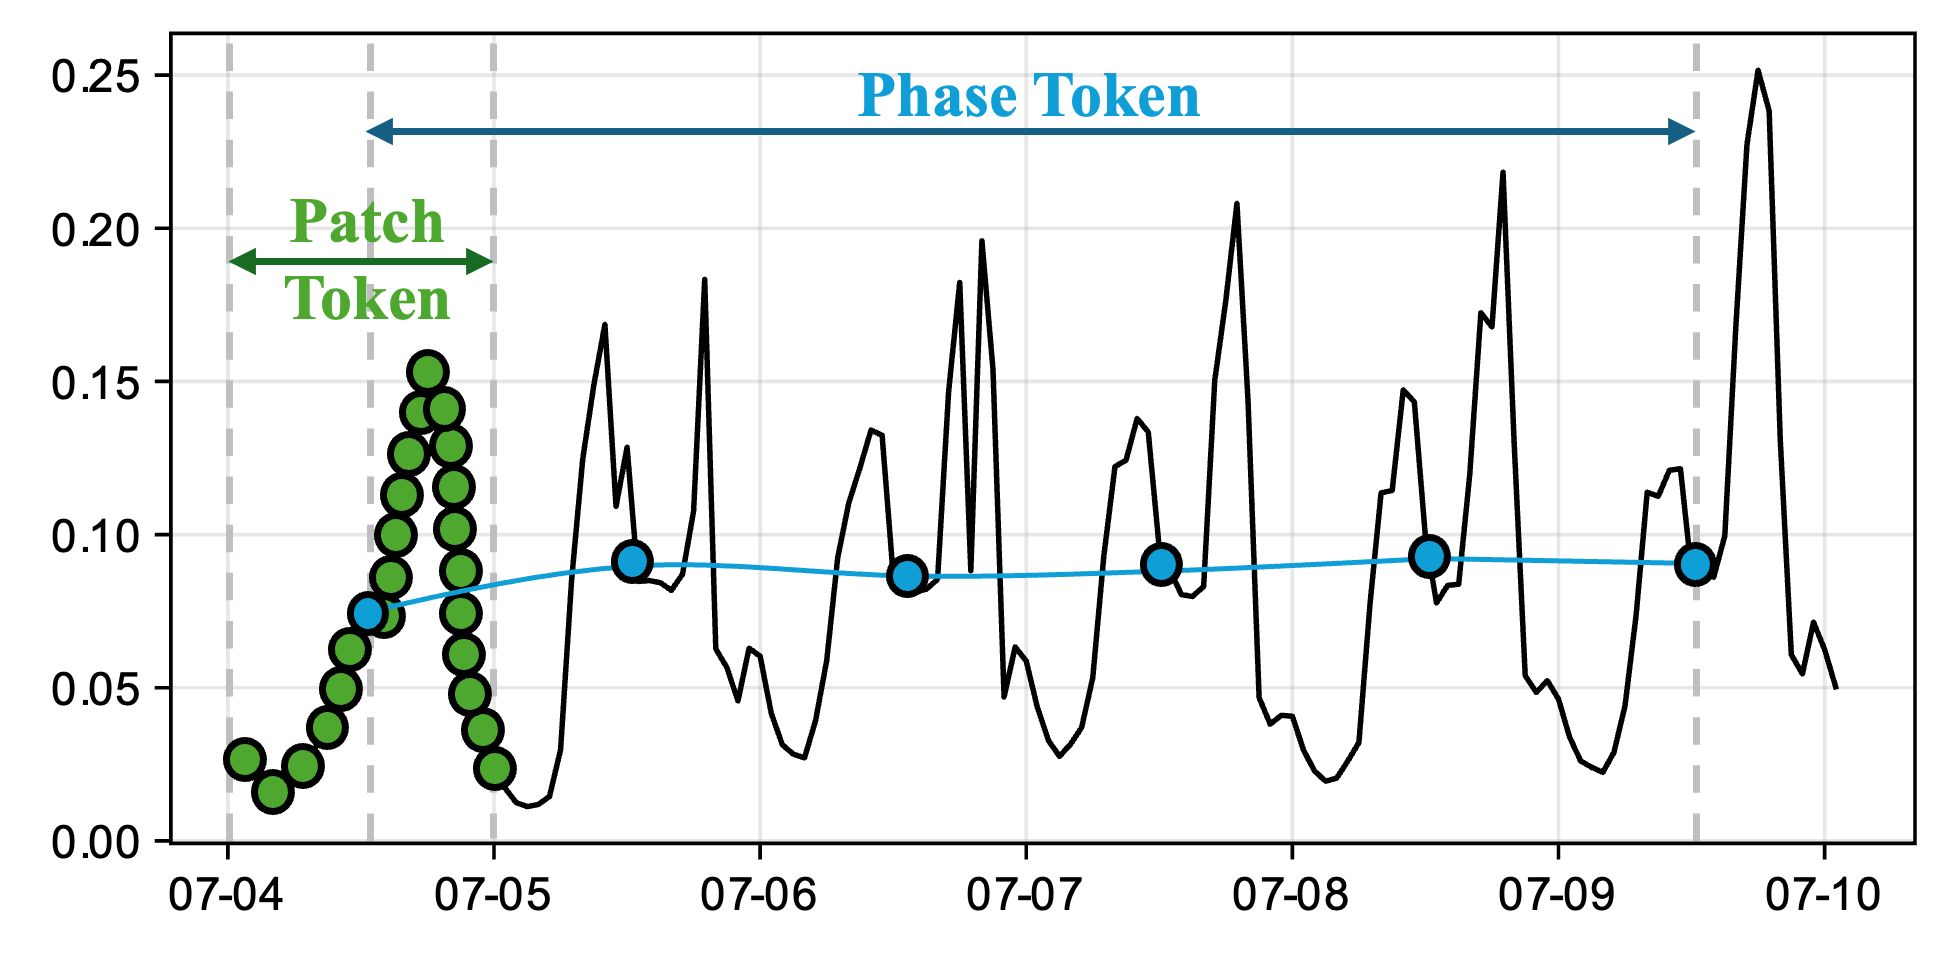
\includegraphics[width=\linewidth]{figures/phase_token.png}
    \caption{\blue{分块标记与相位标记。}}
    \label{fig:phase_token}
  \end{subfigure}
  \hfill
  \begin{subfigure}[t]{0.49\textwidth}
    \centering
    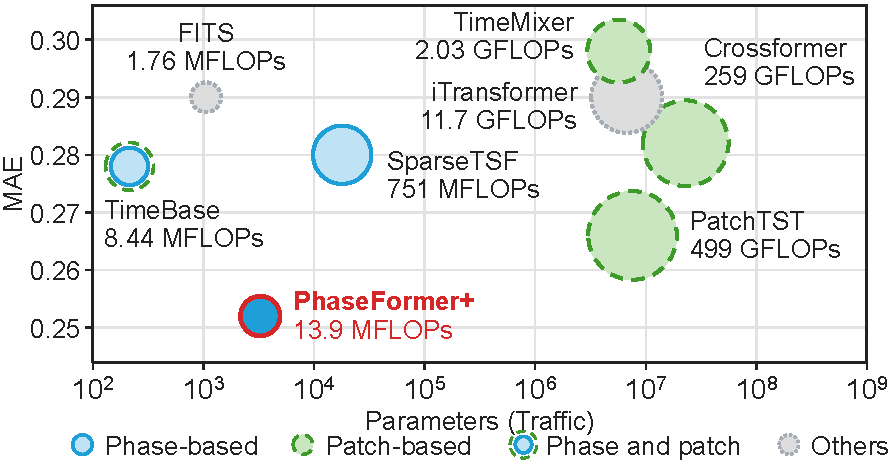
\includegraphics[width=\linewidth]{figures/efficiency_plot.pdf}
    \caption{\blue{精度与效率。}}
    \label{fig:efficiency_plot}
  \end{subfigure}
  \caption{\blue{好的标记让极小的模型便已足够。(a)~分块标记保存连续取值，即其所在周期在当前水平与振幅下的一段周期形状；相位标记收集相继各周期中同一相位处的取值。(b)~Traffic 上的精度与开销：四个预测时域上的平均 MAE 对预测时域 96（输入长度 720）时的参数量绘制；圆点大小随每次预测的 FLOPs 按对数增长，FLOPs 数值印在各名称下方。\sysplus 绘制时计入其相位通路以及水平与振幅通路至多约 2.1K 的参数量，其 FLOPs 取相位通路之值，水平与振幅通路对它增加不足 0.25\%。结合分块与相位的 TimeBase 以双圈标示；FEDformer（MAE 0.400）位于绘图范围之外。}}
  \label{fig:introduction}
\end{figure*}

\blue{
\fakeparagraph{标记应当表示什么}
标记是模型切分序列并在其上进行计算的基本单元，因此标记表示什么，决定了模型必须解开什么。那么，周期序列的标记应当表示什么？将窗口折叠成矩阵 $X$，每个周期一行，周期内每个位置一列，该位置称为其\emph{相位}。周期性意味着各行重复同一个模式，所以窗口首先包含的就是这个模式，即\emph{形状}，例如早高峰与晚高峰。然而重复从不精确，每个周期会在两个方面偏离共同的模式：它处在自己的高度上，即\emph{水平}（一个周期的均值），逐周期漂移，例如某条道路的交通量随周数增长；它还围绕这一水平摆动自己的幅度，即\emph{振幅}，且振幅随水平变动，例如更繁忙的日子里日负荷摆动得更宽。

这三者并不是随意列出的几个特征，而是关于一个重复周期所能说的全部内容：它长什么样、处在哪里、摆动多大。任何一个向量都等于它的均值加上一个尺度乘以一个方向。这里的方向是各周期共有的形状，均值与尺度则是周期之间不同的水平与振幅。就整个窗口而言，这就是一个紧凑结构：一个水平项加一个按振幅缩放的形状，$X\approx\ell\,\one^\top+a\,s^\top$，其中 $\ell$ 为各周期水平，$a$ 为各周期振幅，$s$ 为周期形状。数据印证了这一划分：这一秩二的单一形式在全部七个基准数据集上捕获了归一化输入窗口能量的 78\% 至 93\%（第\ref{sec:mot_tokens}节和图\ref{fig:token_energy}）。各部分占比有所不同：按振幅缩放的形状在 Electricity、Traffic 和 ETTh1 上承载大部分能量，水平则在其余四个数据集上占主导，因此任何一部分都不可省略。周期性窗口整体上是低维的，其每个部分亦然：$X$ 的各列张成一个平面，未来水平是平滑预测时域轮廓的少数几个系数，振幅是跟随水平的每周期一个因子。

现有的主流标记与这一结构并不吻合。分块标记保存连续取值，即其所在周期在当前水平与振幅下的一段周期形状，因此三者中任何一个变化，它都会变化：当通勤习惯改变而交通高峰移动时~\citep{shao2025hutformer,shao2025hyperd,zhou2025feddis}，当水平漂移时，或当繁忙的一天摆动更宽时。要覆盖这一宽泛且不断移动的标记分布，需要更大的表示，这会同时推高参数量与计算量~\citep{shao2025blast}：在 Traffic 上，前两个主成分可解释相位标记 74\% 的方差，而对分块标记只能解释 58\%（第\ref{sec:mot_stability}节）。

\fakeparagraph{为什么部分覆盖并不足够}
三类信息中的每一类与模型相遇，只有三种方式：由一个标记表示它；由标记把它与其他信息混在一起；或者没有任何标记携带它。留下混杂的部分落到网络上，网络必须学会把它解开，因此必须变大；遗漏的内容则丢失，精度随之受损。所以，标记只覆盖三类信息中的一部分的模型，必然要在容量与精度之间付出其中一种代价，无法回避这一选择。这是由部分覆盖本身推出的，而与任何具体模型的细节无关，现有模型也确实分别做出了这两种选择。Autoformer、FEDformer 和 TimeMixer 通过季节部分覆盖形状，并通过趋势覆盖部分水平——趋势是序列的平滑版本，而非逐周期的一个水平——但没有任何机制将季节性摆动与趋势绑定：一个摆动更宽的更繁忙的日子，到达季节性模型时已是一个新的季节性模式；而为每个部分配备的网络（TimeMixer 中还在多个尺度上配备）必须吸收拆分后残留的混合。TimesNet 按其多个周期折叠序列，与我们按单一周期折叠颇为相似，但它把每一折都交给一个深层卷积主干，后者必须自行从形状中分离出水平与振幅，且要同时应对多个周期；而一旦水平与振幅被表示出来，单一周期就已承载窗口能量的 78\% 至 93\%。基于分块的 Transformer 则把三者在每个分块标记中混杂地带入深层注意力堆叠。这些模型选择了容量：标记留下的混杂部分，要用参数量和计算量来偿付。DLinear、FITS 和 SparseTSF 等轻量模型选择了另一侧，保持小规模，但线性映射以同一组权重读取窗口的水平与形状，因此无法让在窗口上平均的形状按由近期周期预测出的水平缩放——这是对窗口两种不同读取之积——而 FITS 与 SparseTSF 在两个传感器网络 Electricity 和 Traffic 上落后（第\ref{sec:exp_results}节）。这些模型无一例外地只覆盖了三类信息的一部分，因而都落在容量与精度的权衡曲线上的某一点（第\ref{sec:related}节）。只有标记覆盖了全部三类，模型才可能在各基准数据集上既很小又准确，而一旦覆盖，留给网络去解开的便所剩无几。

\fakeparagraph{三个标记}
因此我们用三个标记表示一个窗口，每类信息一个，各自取该信息所具有的形式。\emph{相位标记}收集相继各周期中同一相位处的取值，即折叠矩阵的一列（图\ref{fig:phase_token}）；相位标记合起来承载形状。\emph{水平标记}是窗口各周期均值的向量，以最后一个观测值为基准；它承载水平，每周期一个数。\emph{振幅标记}是未来周期形状所按其缩放的因子；由于振幅跟随水平，它由水平标记计算，不需要自己的输入。这一划分源于每类信息各自的变化方式。按上述形式，相位 $p$ 处的相位标记为 $\ell+s_p\,a$：以形状加权的窗口水平与振幅轨迹。当一个窗口的每个周期以相同方式重塑时——例如每天早高峰都提前一小时——只有权重 $s_p$ 变化，因此相位标记在噪声范围内继续张成同一个低维子空间，而分块标记一般会移动到一个新的子空间（定理\ref{thm:stability}），这与 Traffic 上更紧凑的相位标记相一致。相反，水平或振幅的变化会改变 $\ell$ 或 $a$ 本身，从而移动该子空间（第\ref{sec:mot_changes}节）。相位标记因此是形状的稳定载体，而水平与振幅则在其沿周期变化之处被表示。

\fakeparagraph{\sysplus}
在这些标记之上，我们构建了 \textbf{\sysplus}：一个每个标记配一条小通路的预测模型（第\ref{sec:method}节）。\emph{相位通路}将相位标记嵌入一个共享的低维空间，让它们通过少量可学习的标记——路由器——交换信息，其代价随相位数量线性增长，并用一个共享预测器预测每个相位。\emph{水平通路}将水平标记映射到预测时域上的三个固定轮廓：一个偏移、一个倾斜和一个曲率；它绕过相位通路的各层归一化，因此它预测的水平不受其约束，下文的包络将这一点说得更精确。\emph{振幅通路}用由水平计算的因子重新缩放相位表示的周期内部分；由于这一缩放在各相位上中心化，它可证明地保持每个未来周期均值不变，因此振幅通路绝不会移动水平通路所设定的水平。两个门控融合相位与水平预测，一个用于周期水平，一个用于周期内形状。

\fakeparagraph{统一的低维视角}
三个标记并非三个彼此独立的装置。它们是窗口单一低维形式的三个因子，$X\approx\ell\,\one^\top+a\,s^\top$，而每条通路都取其因子的低维形式（第\ref{sec:theory}节）：相位通路预测形状 $s$，水平通路通过少数几个轮廓系数预测水平项，振幅通路通过水平预测因子 $a$。理论确立了这一对应关系的两半。第一，水平与振幅需要各自专属的通路。相位标记包含水平与振幅的轨迹，且相位通路具有足够表达能力：以合适的权重，它能实现 Holt--Winters 型的季节性预测模型~\citep{winters1960forecasting}，跟随水平漂移。然而对任意固定权重，其预测器读取的是层归一化的输出，即一个大小有界的向量，因此预测水平停留在一个固定区间内，周期内振幅低于一个固定上界。这些\emph{水平包络}与\emph{振幅包络}可由权重计算得到，需要超出包络的窗口会遭遇误差下界。更多深度、更多路由器或更多注意力头都无法消除它们：附加容量不能替代缺失的标记。

第二，包络之外的部分本身也是低维的。在标准季节性模型下，缺失的水平是每窗口少数几个数，各自乘以一个固定的预测时域轮廓；缺失的振幅是由水平驱动的一个因子缩放的周期形状；这些恰好是水平通路与振幅通路的形式。训练后的模型印证了这一点。要在每个窗口上追踪最近一个周期的水平，所需的水平包络会宽于训练权重在任何基准数据集上发展出的包络；而水平包络恰在 ETTh2、ETTm2 和 Weather 上约束生效，那里 12\% 至 21\% 的测试窗口需要包络之外的水平——这些正是水平标记收益最大的数据集。在 ETTh1 上，振幅包络约束生效而水平包络几乎不生效，带来收益的是振幅标记（第\ref{sec:exp_theory}节和第\ref{sec:exp_ladder}节）。

\fakeparagraph{结果}
\sysplus 在七个基准数据集中的六个上取得了相对八个基线的最佳平均 MSE（FITS 在 ETTh2 上领先），同时比基于分块的 Transformer 小若干个数量级。其优势为：在 Electricity 上领先 iTransformer 3.6\%，在两个传感器网络上领先小型跨周期预测模型 SparseTSF~\citep{lin2024sparsetsf} 与 TimeBase~\citep{huang2025timebase} 约 5\% 至 6\%（第\ref{sec:exp_results}节）。每个标记都名副其实：在同一训练协议下的标记消融中，\sysplus 在七个数据集均值中的五个上优于其仅相位变体，幅度最高达 3.3\%，在其余两个上与之相差不超过 0.3\%；其四项最大收益恰落在四个包络约束生效的数据集上（第\ref{sec:exp_ladder}节）。在最大的基准数据集 Traffic 上，相位通路需要约 1.2K 参数量，并将 PatchTST 和 Crossformer 的 FLOPs 削减约 99.99\%；水平与振幅通路至多增加约 2.1K 参数量，其中大部分是逐通道门控，在 Traffic 和 Electricity 上增加的 FLOPs 不足 0.25\%（图\ref{fig:efficiency_plot}与第\ref{sec:exp_efficiency}节）。预测周期性传感器数据流因此并不需要现有模型的复杂性：有了覆盖形状、水平与振幅的标记，几千参数量的模型便已足够；而由于一个共享模型服务每个传感器，计算上的每一点节省都会在网络每个传感器上、每次更新时重复兑现。

我们做出四项贡献：
\begin{enumerate}[leftmargin=2em]
\item \emph{以标记为中心的预测模型设计原则。}我们表明，周期序列的一个窗口携带三类信息——其各周期的形状、水平与振幅——它们构成一个秩二结构，在七个基准数据集上捕获归一化窗口能量的 78\% 至 93\%，且在其中五个数据集上振幅与水平相耦合。当标记覆盖全部三类信息时，预测模型既小又精确（第\ref{sec:motivations}节）。

\item \emph{\sysplus。}我们设计遵循这一结构的相位、水平与振幅标记，并各用一条小通路处理：一条跨相位路由并配共享预测器的相位通路，一条将水平标记映射到固定预测时域轮廓的水平通路，以及一条用水平重新缩放周期形状、且可证明地保持每个未来周期均值不变的振幅通路（第\ref{sec:method}节）。

\item \emph{三个标记的统一低维视角。}我们证明：当每个周期以相同方式重塑时，相位标记持续张成一个固定子空间，而分块标记一般不会；对固定权重，相位通路将预测水平与振幅限制在两个可由权重计算的包络内，超出包络则误差存在一个任何附加深度、路由器或注意力头都无法消除的下界；并且在标准季节性模型下，包络之外的部分恰好取水平通路与振幅通路的低维形式（第\ref{sec:mot_stability}节和第\ref{sec:theory}节）。

\item \emph{好标记胜过附加复杂性的证据。}以相位通路约 1.2K 参数量、水平与振幅至多再加约 2.1K 参数量，\sysplus 在七个基准数据集中的六个上取得了相对八个基线的最佳平均 MSE。在同一协议下逐个标记构建，它在七个数据集中的五个上取得收益，而从训练权重读出的包络恰好定位了水平标记收益最大的数据集（第\ref{sec:exp}节）。
\end{enumerate}

\fakeparagraph{与会议版本的关系}
本文是我们会议论文~\citep{niu2026phaseformer}的扩展版本，后者引入了相位标记与相位通路。水平与振幅标记、它们的通路、三个标记的统一低维视角（第\ref{sec:mot_tokens}节、第\ref{sec:mot_changes}节与第\ref{sec:theory}节），以及检验它们的实验，均为新增内容。
}

\section{\blue{相关工作}}
\label{sec:related}

\blue{
周期序列的形状、水平与振幅此前都曾被建模，但分散在不同的工作脉络中，没有任何一条脉络覆盖全部三者。一条脉络若把两类信息留在一起，其网络就必须变大去分离它们；若遗漏一类，其预测就会损失精度。\sysplus 用其标记覆盖全部三类信息，正是这种覆盖让它得以很小。下面依次回顾分解、标记与跨周期模型，最后落到传感器网络规模的预测——那里最需要小模型。

\fakeparagraph{分解}
将序列分解为可解释的部分是一个悠久的传统：从 STL~\citep{cleveland1990stl} 的趋势、季节与余项成分，到 Holt--Winters 预测~\citep{holt2004forecasting,winters1960forecasting,hyndman2021fpp3}，其乘性形式用水平缩放季节分量。深度预测模型将这种拆分内置到架构之中，其中两个工作定义了这条脉络。Autoformer~\citep{wu2021autoformer} 在每一层内部把滑动平均趋势与季节部分分开，并用自相关建模季节部分；FEDformer~\citep{zhou2022fedformer} 沿袭这一做法，改用多个滑动平均的混合与频域注意力。TimeMixer~\citep{timemixer24} 把这一思路推得最远：它将序列下采样到多个尺度，把每个尺度分解为季节与趋势部分，季节部分由细到粗、趋势部分由粗到细地混合，并对每个尺度一个预测器给出的预测求和。DLinear~\citep{zeng2023dlinear} 对每个部分各施加一个线性映射，N-BEATS~\citep{oreshkin2020nbeats} 在多项式趋势基与傅里叶季节基上展开预测，CycleNet~\citep{lin2024cyclenet} 为每个通道学习一个循环周期并预测残差。它们都与本文共享同一个前提：序列的各个部分不应在一个不加区分的表示中学习。

\fakeparagraph{分解的不足}
然而，分解沿时间切分序列，再把各部分相加。用第\ref{sec:mot_tokens}节的形式 $X\approx\ell\,\one^\top+a\,s^\top$ 来看，其季节部分承载形状，趋势替代水平，但趋势是一条随时间变化的平滑曲线，而不是每周期一个数；振幅则根本没有自己的成分：没有任何机制把季节性摆动与趋势绑定，一个摆动更宽的更繁忙的日子，到达季节性模型时已是一个新的季节性模式。拆分后残留的混合落到每个部分的网络上，网络必须变大才能把它解开，如 Autoformer、FEDformer 和 TimeMixer；若这个网络只是一个线性映射，如 DLinear，它就解不开，预测只能以精度为代价。因此，部分覆盖迫使模型在容量与精度之间二选一。\sysplus 覆盖全部三类信息——每周期一个水平、一个由水平驱动的振幅、承载形状的相位标记——仅凭数千参数，就在每个数据集的两项指标上都比 FEDformer 和 TimeMixer 更准确（第\ref{sec:exp_results}节）。

\fakeparagraph{标记与跨周期模型}
标记决定了预测模型必须解开什么。Autoformer 和 FEDformer 将每个时间步嵌入为一个标记，iTransformer~\citep{liu2023itransformer} 则以一个变量的整条序列为标记。PatchTST~\citep{nie2023patchtst}、Crossformer~\citep{zhang2023crossformer} 和 PatchMLP~\citep{tang2025patchmlp} 取连续值构成的分块，分块混合了一个周期的形状、水平与振幅，因此必须由深层注意力或 MLP 堆叠来分离它们；\sysplus 的路由器沿袭了 Crossformer 的路由标记与 Perceiver~\citep{jaegle2021perceiver} 的潜在数组。TimesNet~\citep{wu2023timesnet} 按其主导周期折叠序列，与 \sysplus 按单一周期折叠相似，但它把折叠结果交给深层二维卷积，由后者自行从形状中分离出水平与振幅。跨周期模型利用折叠保持小规模：SparseTSF~\citep{lin2024sparsetsf} 用一个共享线性映射预测每个相位，TimeBase~\citep{huang2025timebase} 预测周期长度片段的少数几个基成分。二者都没有为水平或振幅提供标记，而且由于是线性的，都无法让在窗口上平均的形状按由近期周期预测出的水平缩放——这一乘积正是 \sysplus 的振幅通路所构成的（命题\ref{prop:modulation}）。这些工作都没有把标记应表示的内容区分为形状、水平与振幅；\sysplus 做到了，并证明了跨周期分组得到的标记何时保持在固定子空间中（定理\ref{thm:stability}）。

\fakeparagraph{传感器网络规模的预测}
Graph WaveNet~\citep{wu2019graphwavenet}、MTGNN~\citep{wu2020mtgnn}、AGCRN~\citep{bai2020agcrn} 和 D2STGNN~\citep{shao2022decoupled} 等时空图模型在传感器之间传递消息，BigST~\citep{han2024bigst}、LightCTS~\citep{lai2023lightcts} 和 STID~\citep{shao2022stid} 则降低其开销；\sysplus 与这一脉络互补，因为它缩小的是服务每个传感器的通道独立模型，空间模型可以构建在它之上。另一条路线通过限制模型来保持逐序列模型的小规模：DLinear 与 FITS~\citep{fits2024} 限于线性映射，FilterNet~\citep{filternet2024} 限于频域滤波器，SSCNN~\citep{deng2024parsimony} 限于简约的分解。\sysplus 则靠覆盖变小，而它所覆盖的结构在传感器网络上最强：振幅在 Traffic 的 862 个道路传感器与 Electricity 的 321 个电表上最紧密地跟随水平（第\ref{sec:mot_changes}节），\sysplus 也正是在这两个数据集上领先 SparseTSF 与 TimeBase 约 5\% 到 6\%（第\ref{sec:exp_results}节）。一个模型服务的传感器越多，完整的标记回报越大。
}

\section{\blue{标记必须表示什么}}
\label{sec:motivations}
\blue{本节分三步回答：预测模型的标记必须承载什么。周期序列的一个窗口由三个部分组成——周期的形状、水平与振幅——每个基准数据集都需要全部三者（第\ref{sec:mot_tokens}节）。相位标记能稳定地承载形状，分块标记则不能（第\ref{sec:mot_stability}节）。相位标记无法稳定地承载水平与振幅，因此二者需要自己的标记；又由于振幅跟随水平，一个水平标记就能同时驱动两者（第\ref{sec:mot_changes}节）。}

\blue{
\subsection{一个窗口，三个部分}
\label{sec:mot_tokens}

\begin{figure}[t]
\centering
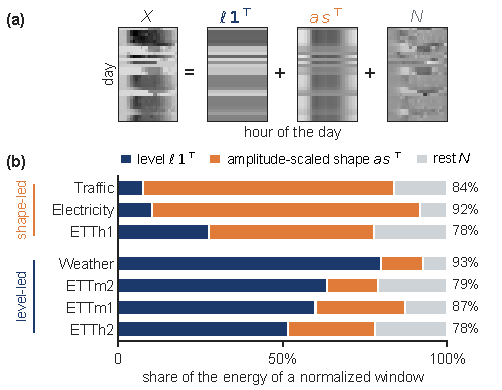
\includegraphics[width=\linewidth]{figures/token_energy.pdf}
\caption{窗口是一个水平项加一个按振幅缩放的形状。(a)~一个归一化的 Traffic 窗口（每天一行）及其在\equref{eq:three_parts}中的三个项。(b)~三个正交项的能量占比，在测试窗口上取平均；数字为前两项之和。橙色在三个数据集上占主导，深蓝在其余四个上占主导。}
\label{fig:token_energy}
\end{figure}

将周期序列的一个归一化窗口折叠成矩阵 $X\in\mathbb R^{D\times H}$，每个周期一行，周期内每个位置一列，该位置称为其\emph{相位}（第\ref{sec:method}节）。各行重复同一个模式，但并不精确：有些周期整体偏高，有些摆动更大。因此三个量就能描述一个窗口：\emph{形状} $s\in\mathbb R^H$，即所有周期共有的模式；每个周期的\emph{水平} $\ell_k$，即其均值；每个周期的\emph{振幅} $a_k$，即其围绕水平摆动的幅度。每个周期等于它的水平加上它的振幅乘以形状，于是
\begin{equation}
X=\ell\,\one^\top+a\,s^\top+N ,
\label{eq:three_parts}
\end{equation}
即一个\emph{水平项}加一个\emph{按振幅缩放的形状}，其中 $\ell,a\in\mathbb R^D$，$N$ 为余项。这里 $\ell$ 为各周期均值，$s$ 均值为零、均方根为一，$a\,s^\top$ 是对周期内部分 $X-\ell\,\one^\top$ 的最佳秩一拟合，因此三项两两正交。去掉余项后，窗口的秩至多为二：它的各列位于 $\ell$ 与 $a$ 张成的平面中，各行位于 $\one$ 与 $s$ 张成的平面中。

真实窗口与这一形式很接近：在每个数据集上，水平项与按振幅缩放的形状承载窗口 78\% 至 93\% 的能量（图\ref{fig:token_energy}）。由于窗口经过归一化，水平项衡量的是水平在窗口内漂移的程度，而不是整体偏移。哪一项占主导取决于数据：按振幅缩放的形状在 Electricity、Traffic 和 ETTh1 上占主导，水平项在其余四个数据集上占主导。因此两项都不能舍弃。

\fakeparagraph{要点}
\emph{窗口是一个水平项加一个按振幅缩放的形状，每个基准数据集都需要这两项。}预测模型的标记必须承载形状、水平与振幅。}

\begin{figure}[t]
\centering
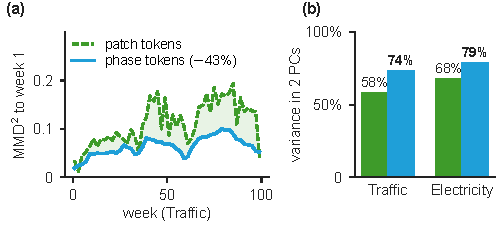
\includegraphics[width=\linewidth]{figures/token_geometry.pdf}
\caption{\blue{相位标记稳定且紧凑地承载形状。(a)~Traffic 上每周的标记相对第一周的漂移（MMD$^2$）；越低越稳定。(b)~前两个主成分所解释的方差；越高越紧凑。绿色：分块标记；蓝色：相位标记。}}
\label{fig:phase_token_comparison}
\end{figure}

\subsection{\blue{形状：相位标记稳定地承载它}}
\label{sec:mot_stability}

\blue{哪种标记能承载这些部分？由\equref{eq:three_parts}，\emph{分块标记}是 $X$ 的一行，$\ell_k\one+a_k\,s$：形状与 $\one$ 一起张成它所在的平面。\emph{相位标记}是一列，$\ell+s_p\,a$：它位于 $\ell$ 与 $a$ 张成的平面中，形状只通过权重 $s_p$ 决定它在平面中的位置。标记还必须\emph{稳定地}承载其部分：当该部分变化时，标记应停留在基于过去窗口拟合的模型所预期的位置。

考虑形状的变化，例如通勤习惯改变时，每个周期的早晚高峰都同样地移动。相位标记只在其平面内移动；分块标记所在的平面则会转动。真实数据同时呈现了这两种效应。}

\fakeparagraph{洞察 1：在 Traffic 上，相位标记的漂移更小}
\blue{在 Traffic 上，我们用平方最大均值差异（MMD$^2$）~\citep{ouyang2021mmd} 衡量每周的标记相对第一周的标记漂移了多远；相位标记的漂移比分块标记低 43\%（图\ref{fig:phase_token_comparison}(a)）。}

\fakeparagraph{洞察 2：相位标记更紧凑}
\blue{前两个主成分在 Traffic 上解释相位标记 74\% 的方差，在 Electricity 上解释 79\%，而分块标记分别只有 58\% 和 68\%（图\ref{fig:phase_token_comparison}(b)）：相位标记集中在 $\ell$ 与 $a$ 张成的平面中，而分块标记与输入窗口一样可以从周期中的任一相位开始，因此散布在形状的许多平移副本上。}

\blue{定理\ref{thm:stability}对任意低秩窗口 $X=AG^\top+N$ 证明了这一机制；\equref{eq:three_parts}是其中 $A=[\ell,\,a]$、$G=[\one,\,s]$ 的情形，公共形状变化把 $X$ 变为 $XS^\top$。证明见电子补充材料。}

\begin{theorem}[\blue{相位标记的稳定性}]
\label{thm:stability}
\blue{设 $X=AG^\top+N$，其中 $A$、$G$ 与 $SG$ 的秩均为 $r$；设 $X'=XS^\top+R$，$R$ 为小扰动。记 $\mathcal U_r$ 与 $\mathcal V_r$ 分别为相位标记与分块标记的前 $r$ 维子空间，$d$ 为子空间之间的距离，$\delta_{\min}>0$ 为信号的谱间隙，$\eta=C(\|N\|_2+\|NS^\top\|_2+\|R\|_2)/\delta_{\min}$，$C$ 为普适常数。则}
\begin{enumerate}[leftmargin=2em]
\item \blue{$d\big(\mathcal U_r(X),\mathcal U_r(X')\big)\le\eta$：相位标记保持其子空间，无噪声时严格不变；}
\item \blue{$d\big(\mathcal V_r(X),\mathcal V_r(X')\big)\ge d\big(\mathrm{Col}(G),\mathrm{Col}(SG)\big)-\eta$：形状变化使 $\one$ 与 $s$ 张成的平面转动多少，分块标记就移动多少。}
\end{enumerate}
\end{theorem}

\fakeparagraph{要点}
\blue{\emph{相位标记稳定地承载形状；分块标记做不到。}另一面是：相位标记的平面由 $\ell$ 与 $a$ 张成，因此仍会移动相位标记的，是水平或振幅的变化。}

\blue{
\subsection{水平与振幅：需要自己的标记}
\label{sec:mot_changes}

\begin{figure}[t]
\centering
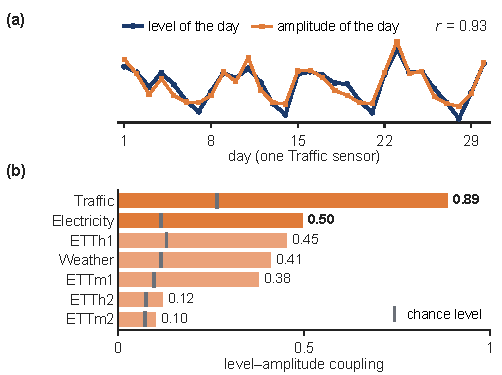
\includegraphics[width=\linewidth]{figures/coupling.pdf}
\caption{越繁忙的日子摆动越大。(a)~某个 Traffic 传感器每天的水平与振幅，已标准化。(b)~各数据集测试窗口上的水平–振幅耦合；深色：两个传感器网络；刻度：偶然水平。}
\label{fig:coupling}
\end{figure}

在一个窗口内，水平与振幅逐周期变化：一条道路有些天比另一些天更繁忙，而在繁忙的日子里，早晚高峰远高于夜间（图\ref{fig:coupling}(a)）。因此，随着窗口向前移动，它会带来新的轨迹 $\ell$ 与 $a$。在折叠后的窗口中，这两种变化为
\begin{equation}
\underbrace{X+\delta\,\one^\top}_{\text{水平漂移}},
\qquad
\underbrace{X+\operatorname{diag}(\alpha\ell)\,(X-\ell\,\one^\top)}_{\text{跟随水平的振幅}},
\label{eq:cycle_axis_changes}
\end{equation}
其中 $\delta\in\mathbb R^D$ 平移各周期的水平，$\alpha$ 决定摆动随水平增长的强度。它们把 $\ell$ 换成 $\ell+\delta$，把 $a$ 换成 $(\one+\alpha\ell)\odot a$。两者改变的恰是张成相位标记平面的那两条轨迹，因此一般都会移动这个平面。只读取相位标记的模型必须在每个窗口中重新估计水平与振幅，第\ref{sec:theory}节表明，在固定权重下，它只能在两个可由权重计算的包络之内做到这一点。因此，水平与振幅需要自己的标记。

不过，二者不必拥有两个彼此独立的标记。把这两种变化结合起来，加上噪声和以随机游走漂移的水平，就得到原始序列的一个简单季节模型，
\begin{equation}
X_{kp}=\ell_k+(1+\alpha\ell_k)\,s_p+e_{kp},
\qquad
\ell_k=\ell_{k-1}+\eta_k,
\label{eq:mult_model}
\end{equation}
其中形状 $s$ 均值为零、均方根为一，噪声为高斯噪声。当 $\alpha=0$ 时，它是加性季节随机游走模型；当 $\alpha\neq0$ 时，摆动随水平增大（$\alpha>0$）或减小（$\alpha<0$），我们仿照 Holt--Winters 预测的乘性形式~\citep{winters1960forecasting}，称之为乘性模型。此时振幅 $\one+\alpha\ell$ 是水平的函数，对水平的预测也就给出了振幅，因此一个水平标记就能同时驱动两者。洞察~3 表明真实数据正是如此。

\fakeparagraph{洞察 3：振幅跟随水平}
在图\ref{fig:coupling}(a) 的 Traffic 窗口中，30 天的水平与振幅同起同落（$r=0.93$）。为检验每个数据集，我们在每个通道的每个测试窗口中计算二者的相关系数，并在每个通道的各窗口上对带符号的相关系数取平均，使偶然相关相互抵消；再对这些通道平均值的绝对值取平均，因为符号在通道内稳定，但在 ETTh1 和 ETTm1 上因通道而异。所得的\emph{水平–振幅耦合}在七个基准数据集中的五个上远高于其偶然水平（即把水平与振幅取自不同窗口时的同一统计量），并在两个传感器网络上最强：Traffic 上为 0.89，Electricity 上为 0.50（图\ref{fig:coupling}(b)）。ETTh2 和 ETTm2 的耦合最弱，但在这两个数据集上水平本身主导窗口（图\ref{fig:token_energy}(b)），因此同样需要水平标记。电子补充材料给出细节，并表明训练期与验证期上的排序相同。

\fakeparagraph{要点：一个形式，三个标记}
\emph{水平与振幅逐周期变化，而且振幅跟随水平。}因此，\equref{eq:three_parts}的每个部分都有自己的标记（表\ref{tab:three_tokens}）：形状由相位标记承载，水平由每周期一个数的水平标记承载，振幅由从水平标记计算出的振幅标记承载。每个部分一个标记，就没有留给网络去解开的混杂；三个部分全部覆盖，就没有任何遗漏。第\ref{sec:method}节为每个标记构建一条小通路，第\ref{sec:theory}节说明为什么每条通路都是必要的，以及为什么三者合起来就足够。

\begin{table}[t]
\centering
\caption{一个形式，三个标记。}
\label{tab:three_tokens}
\footnotesize
\setlength{\tabcolsep}{2.5pt}
\begin{tabular}{@{}l l p{0.2\linewidth} p{0.31\linewidth} l@{}}
\toprule
部分 & 因子 & 如何变化 & 紧凑形式 & 标记 \\
\midrule
形状 & $s$ & 在每个周期中同样变化 & 一个向量；相位标记保持其子空间（定理~\ref{thm:stability}） & 相位 \\
水平 & $\ell$ & 逐周期变化 & 每周期一个数 & 水平 \\
振幅 & $a$ & 随水平变化 & 每周期一个数，由水平计算（洞察~3） & 振幅 \\
\bottomrule
\end{tabular}
\end{table}
}


\section{\blue{\sysplus：每个标记一条小通路}}
\label{sec:method}

\blue{\sysplus 是一个拥有三个标记与三条小通路的模型，每条通路预测第\ref{sec:motivations}节中窗口形式 $X\approx\ell\,\one^\top+a\,s^\top$ 的一部分（图\ref{fig:la_overview}）。\emph{相位通路}是一个基于相位的路由 Transformer，读取相位标记并预测每个相位，从而得到形状 $s$（第\ref{subsec:phase-network}节）。\emph{水平通路}读取水平标记，经由一个到固定偏移、倾斜与曲率轮廓的秩三映射预测水平项（第\ref{sec:ext_level}节）。\emph{振幅通路}以水平驱动的因子缩放相位预测的周期内部分（第\ref{sec:ext_modulation}节）。随后两个门控将已被振幅通路重缩放的相位预测与水平通路预测融合（第\ref{sec:ext_init}节）。因此一个水平标记同时驱动水平与振幅，三条通路产生一个预测。这些通路之所以小，是因为各自承载的内容是低维的：在最大的基准 Traffic 上，相位通路约需 1.2K 参数，水平与振幅通路至多再增加约 2.1K（第\ref{sec:complexity}节与第\ref{sec:exp_efficiency}节）。}

\blue{\fakeparagraph{问题设定}
\sysplus 是通道独立的}~\citep{nie2023patchtst, zeng2023dlinear}\blue{：一个共享模型分别预测每个传感器的序列，因此它在传感器网络上的代价等于单传感器代价乘以传感器数量。以下我们省略通道维；数据集的 $C$ 个通道共享一个模型。}预测的目标是从输入序列 $\mathbf{X}\in\mathbb{R}^{L_{\text{in}}}$ 预测未来轨迹 $\mathbf{Y}\in\mathbb{R}^{L_{\text{out}}}$，其中 $L_{\text{in}}$ 与 $L_{\text{out}}$ 分别表示输入长度与输出长度。

\begin{figure*}[t]
\centering
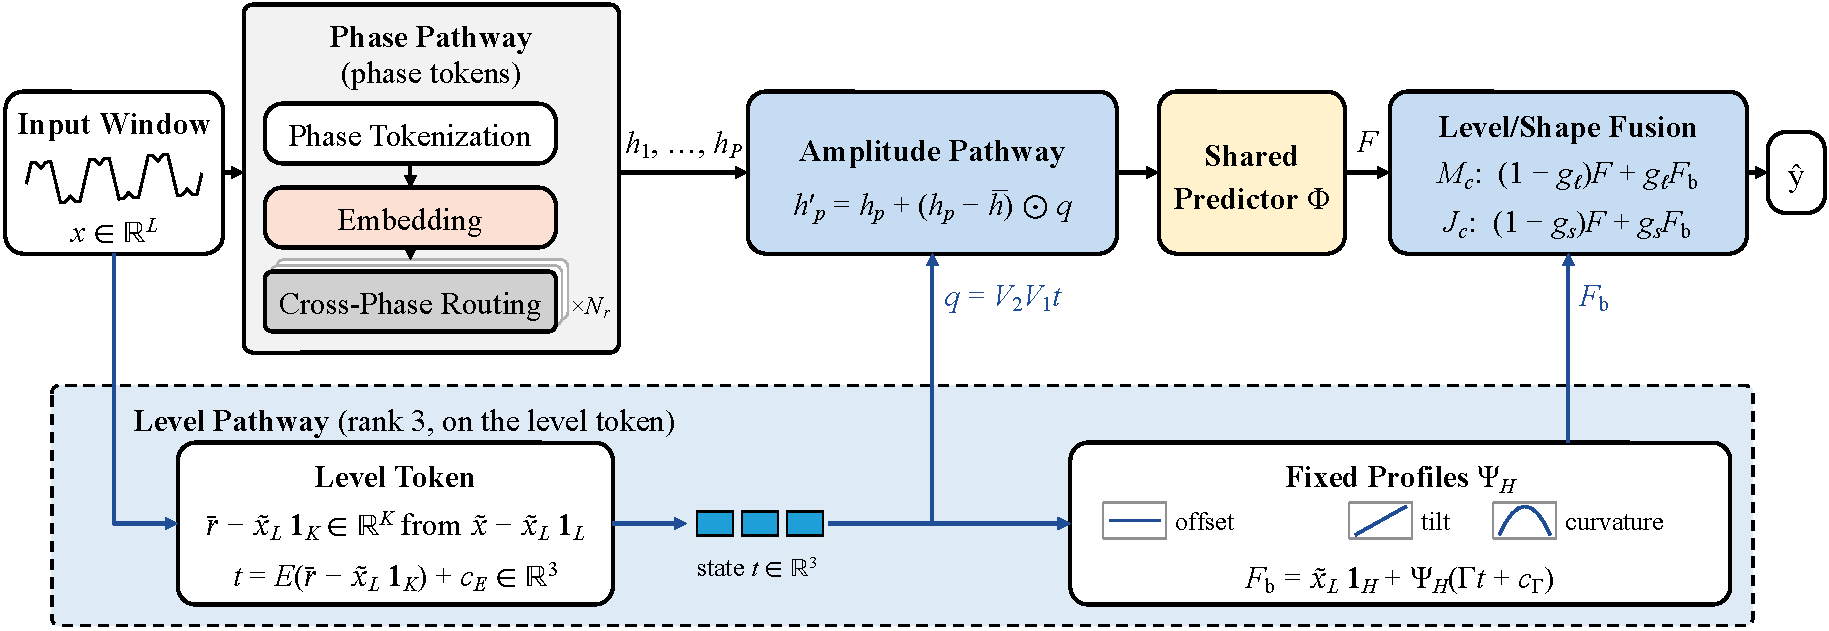
\includegraphics[width=\textwidth]{figures/la_overview.pdf}
\caption{\blue{\sysplus：三个标记、三条小通路、一个预测。相位通路嵌入相位标记，并通过 $N_r$ 层跨相位路由层将其精炼为最终相位隐变量 $h_1,\dots,h_P$；在振幅通路对其重缩放之后，共享预测器 $\Phi$ 将其解码为相位预测 $F$。水平通路（下方）将水平标记（即锚定的周期均值）映射为三维状态 $t$，并将其映射到偏移、倾斜与曲率轮廓 $\Psi_H$ 上，得到水平通路预测 $F_{\mathrm b}$。振幅通路由同一状态 $t$ 计算振幅标记 $q$，并以 $\one+q$（在相位上中心化）缩放相位隐变量的周期内部分。两个门控融合 $F$ 与 $F_{\mathrm b}$ 的周期水平与周期内形状。图\ref{fig:overview}给出相位通路的细节。}}
\label{fig:la_overview}
\end{figure*}

\begin{figure*}[t]
    \centering
    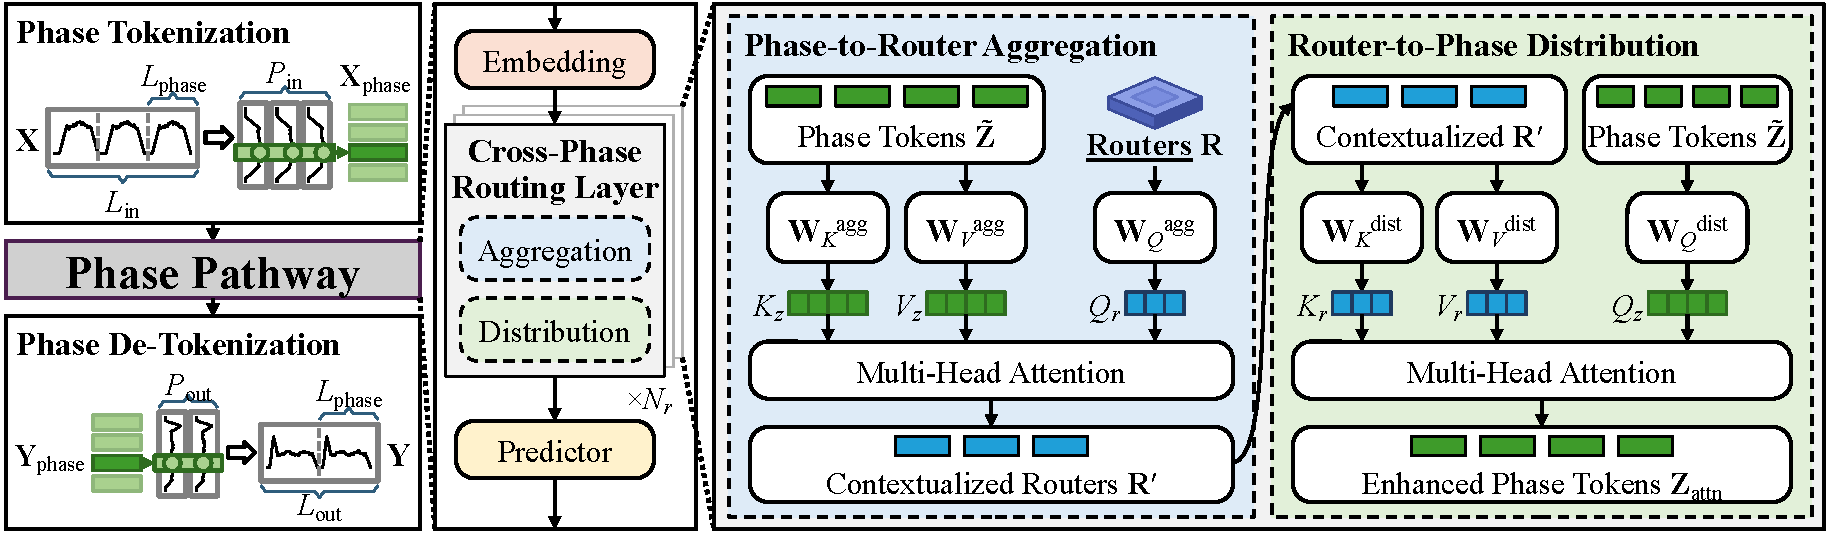
\includegraphics[width=\textwidth]{figures/phaseformer_overview.pdf}
    \caption{\blue{\sysplus 的相位通路：相位标记化与去标记化（左）；嵌入层、$N_r$ 层跨相位路由层与共享预测器（中）；以及路由层内部，若干路由器从所有相位收集消息再分发回去（右）。}}
    \label{fig:overview}
\end{figure*}

\subsection{\blue{从窗口到三个标记}}
\label{subsec:preprocessing}
\fakeparagraph{归一化与去归一化}
遵循 \cite{kim2021reversible}，我们用输入的估计均值与标准差对其进行归一化，并将预测去归一化到原始尺度。\blue{该归一化（RevIN）将均值为 $\mu$、标准差为 $\sigma$ 的输入窗口 $x$ 映射为 $\tilde x=(x-\mu\one)/\sigma$，使 $\one^\top\tilde x=0$；该坐标系下的预测 $\hat{\tilde y}$ 去归一化为 $\hat y=\mu\one+\sigma\hat{\tilde y}$。}

\fakeparagraph{相位标记化与去标记化}
相位标记化将一维输入序列变换为二维的相位–周期矩阵，以供\blue{后续}处理。
反之，相位去标记化将预测的相位–周期矩阵重构回一维输出序列。
\revised{\blue{记 $L_{\text{phase}}$ 为周期长度，即一个周期所含的步数，我们也称其为相位长度；它由频域分析估计（\secref{sec:phase_length}）并保持固定。}}

为确保输入序列长度是 $L_{\text{phase}}$ 的整数倍，我们循环填充序列至长度 \blue{$P_{\text{in}}L_{\text{phase}}$}，其中 $P_{\text{in}} = \left\lceil \frac{L_{\text{in}}}{L_{\text{phase}}} \right\rceil.$ \blue{是 $L_{\text{phase}}$ 整数倍的输入长度无需填充，建议尽可能采用。}
如\figref{fig:overview}所示，填充后的序列 $\mathbf{X}$ 随后被重塑为相位–周期矩阵 $\mathbf{X}_{\text{phase}} \in \mathbb{R}^{L_{\text{phase}} \times P_{\text{in}}}$，其中每个元素 \blue{$\mathbf{X}_{\text{phase}}[p, k]$ 对应第 $k$ 个周期中第 $p$ 个相位处的观测}。
\blue{去标记化将这一重塑逆转。}

\blue{
\fakeparagraph{记号}
我们简记 $P=\Lp$ 为周期，$K=\Pin$ 与 $K'=\Pout$ 为输入与输出周期数，$L=L_{\text{in}}=KP$ 与 $H=L_{\text{out}}=K'P$ 为输入长度与预测时域。对频域分析找到的周期，实验的输入长度与每个预测时域都是整数个周期，因此不会发生填充。折叠后的归一化窗口 $\tilde X\in\mathbb R^{K\times P}$（即 $\tilde x$ 的相位–周期矩阵的转置）每周期一行；它就是第\ref{sec:motivations}节中 $D=K$ 个周期、$H=P$ 个相位的矩阵 $X$，此后 $H$ 表示预测时域。第\ref{subsec:phase-network}节与第\ref{sec:complexity}节使用符号 $\Lp$、$\Pin$ 与 $\Pout$，它们同样适用于填充后的输入。

\fakeparagraph{三个标记}
三个标记对应\equref{eq:three_parts}的三个部分。
\begin{itemize}[leftmargin=1.2em,itemsep=0.1em,topsep=0.2em]
\item \emph{相位标记}是 $\tilde X$ 的列 $\tilde x_p\in\mathbb R^K$，每个相位一个。除去噪声，每个列都等于 $\ell+s_p\,a$，因此它们共同以稳定子空间中坐标的形式携带形状 $s$（第\ref{sec:mot_stability}节）。
\item \emph{水平标记}是窗口的周期水平向量 $\ell$，以窗口的最后一个值 $\tilde x_L$ 为基准度量，
\begin{equation}
\bar r-\tilde x_L\one_K,\qquad \bar r=\tfrac1P\tilde X\one_P\in\mathbb R^K ,
\label{eq:level_token}
\end{equation}
每周期一个数。锚点使其在归一化坐标下具有平移不变性：向 $\tilde x$ 加 $c\one_L$ 不改变水平标记。
\item \emph{振幅标记}是由水平通路的状态计算得到的尺度 $q\in\mathbb R^d$（\equref{eq:la_modulation}）。它是振幅因子 $a$ 的隐变量形式：振幅通路以 $\one+q$ 缩放相位隐变量的周期内部分，因此均匀的 $q=q_1\one_d$ 以单一因子 $1+q_1$ 缩放相位预测的周期内部分。它无需自己的输入，因为振幅跟随水平（第\ref{sec:mot_changes}节）。
\end{itemize}
}

% --------------------------------------------------------------------
\subsection{\blue{相位通路：基于相位的路由 Transformer}}
\label{subsec:phase-network}

\blue{相位通路预测形状。它是一个基于相位的路由 Transformer，是 \sysplus 中唯一使用注意力的部分，由相位标记预测每个相位。}
如\figref{fig:overview}所示，\blue{相位通路}首先对相位标记施加嵌入层，然后通过 \blue{$N_r$ 层}跨相位路由层对其进行精炼，最后经共享预测器将其映射到目标。

% ---------------- embedding ----------------
\subsubsection{嵌入层}
嵌入层将相位标记 $\mathbf{X}_{\text{phase}}$ 投影到低维表示空间，从而能够从常受扰动污染的原始观测中提取信息成分。
形式上，对每个相位索引 \blue{$p \in \{1,\dots,L_{\text{phase}}\}$，其对应的相位标记 $\mathbf{X}_{\text{phase}}[p, :]$}通过\blue{一个仿射映射 $f_{\theta}$，$\theta=(W_e,b_e)$，其权重为 $W_e\in\mathbb R^{d\times\Pin}$、偏置为 $b_e\in\mathbb R^d$，并后接一个 LayerNorm $\LN_e$~\citep{ba2016layernorm}}，被映射为 $d$ 维表示：
\begin{equation}
\mathbf{Z}
= \blue{\LN_e\big(}f_{\theta}\!\left(\mathbf{X}_{\text{phase}}\right)\blue{\big)}\in \mathbb{R}^{L_{\text{phase}}\times d}\blue{.}
\end{equation}

为更好地刻画相位之间的时间顺序，遵循 \cite{liu2023spatio}，我们引入一组可学习的位置嵌入 $\mathbf{E}_{\text{pos}}\in\mathbb{R}^{L_{\text{phase}}\times d}$\blue{，以编码每个相位在周期内的位置}。
这些嵌入逐相位地加到 $\mathbf{Z}$ 上，使每个相位表示都融入其位置信息：
\begin{equation}
\tilde{\mathbf{Z}}=\mathbf{Z}+\mathbf{E}_{\text{pos}}.
\end{equation}
所得的 $\tilde{\mathbf{Z}}$ 随后被送入跨相位路由层，以进行更高层次的特征交互与预测\blue{；在层堆叠中，每一层都以这种方式将自身的位置嵌入加到其输入上}。

% ---------------- Attention ----------------
\subsubsection{跨相位路由层}

\blue{相位标记之间需要交换信息，因为没有任何单个相位标记持有周期形状，而它们张成低维子空间（洞察~2，第\ref{sec:mot_stability}节），因此少量中介即可完成交换。}我们引入一组可学习的路由器 $\mathbf{R}\in\mathbb{R}^{M\times d}$，充任跨相位信息交换的中介。
\revised{
\blue{该设计沿袭已有的路由式架构~\citep{jaegle2021perceiver, zhang2023crossformer}，且路由器利用了}\emph{相位对齐标记固有的低秩结构}。
\blue{跨相位路由将自注意力的二次代价降为关于相位个数的线性代价，同时每个相位仍能与所有其他相位交换信息。}
}

跨相位路由包含两步：
(i) \emph{相位到路由器聚合}，将相位表示中的信息选择性地压缩进紧凑的路由器集合；(ii) \emph{路由器到相位分发}，将聚合的跨相位信息从路由器选择性地传播回相位表示。两步均由交叉注意力实现。

\fakeparagraph{相位到路由器聚合}
路由器关注相位表示以提取上下文信息，得到上下文化路由器嵌入
\blue{$\mathbf{R}'\in\mathbb{R}^{M\times d}$}。
具体而言，路由器充当查询，相位提供键与值。投影矩阵
$\mathbf{W}_Q^{\text{agg}},\mathbf{W}_K^{\text{agg}},\mathbf{W}_V^{\text{agg}}\in\mathbb{R}^{d\times d}$
分别将表示映射到查询、键与值空间：
\begin{equation}
\mathbf{Q}_r=\mathbf{R}\mathbf{W}_Q^{\text{agg}},\quad
\mathbf{K}_z=\tilde{\mathbf{Z}}\mathbf{W}_K^{\text{agg}},\quad
\mathbf{V}_z=\tilde{\mathbf{Z}}\mathbf{W}_V^{\text{agg}}.
\end{equation}
随后通过 \blue{$n_h$} 个头的多头注意力（MHA）得到聚合的路由器嵌入：
\begin{equation}
\blue{\mathbf{R}'}=\mathrm{MHA}\!\left(\mathbf{Q}_r,\mathbf{K}_z,\mathbf{V}_z\right).
\end{equation}

\fakeparagraph{路由器到相位分发}
路由器中聚合的信息随后被重新分发到相位表示，从而实现跨相位信息流动。此步中，相位表示充当查询，路由器提供键与值，得到精炼的相位表示 $\mathbf{Z}_{\text{attn}}$。分发使用投影矩阵 $\mathbf{W}_Q^{\text{dist}}, \mathbf{W}_K^{\text{dist}}, \mathbf{W}_V^{\text{dist}}\in\mathbb{R}^{d\times d}$：
\begin{equation}
\begin{gathered}
\mathbf{Q}_z=\tilde{\mathbf{Z}}\mathbf{W}_Q^{\text{dist}},\quad
\mathbf{K}_r=\blue{\mathbf{R}'}\mathbf{W}_K^{\text{dist}},\quad
\mathbf{V}_r=\blue{\mathbf{R}'}\mathbf{W}_V^{\text{dist}},\\
\mathbf{Z}_{\text{attn}}=\mathrm{MHA}\!\left(\mathbf{Q}_z,\mathbf{K}_r,\mathbf{V}_r\right).
\end{gathered}
\end{equation}
该机制在恢复相位级分辨率的同时，通过上下文化路由器在相位之间施加一致性。
最终，每个相位表示\blue{都经由路由器、分两步}关注所有其他相位。
\blue{路由层将这两步与残差连接、两个 LayerNorm 和一个 MLP 组合起来：记 $z_p$ 与 $m_p$ 为层输入（首层为 $\tilde{\mathbf Z}$）与 $\mathbf Z_{\text{attn}}$ 的第 $p$ 行，它计算 $o_p=\LN_1(z_p+m_p)$ 并输出 $h_p=\LN_2\big(o_p+\mathrm{MLP}(o_p)\big)$。每个 LayerNorm 在 $d$ 个特征上对其输入做中心化，将其重缩放到单位均方根，并施加可学习的增益 $\gamma_i$ 与偏置 $\beta_i$：$\LN_i(u)=\gamma_i\odot\varsigma+\beta_i$，其中 $\varsigma=J_du/(\|J_du\|^2/d+\epsilon)^{1/2}$、$J_d=I_d-\tfrac1d\one\one^\top$。因此对任意输入有 $\|\varsigma\|<\sqrt d$；又因为 $\LN_2$ 是每个路由层的最后一个操作，每个最终相位隐变量都是有界的。该界把每个相位预测的水平与周期内振幅限制在第\ref{sec:theory}节的两个包络之内，这正是水平标记与振幅标记各自拥有通路的原因：水平通路绕过 $\LN_2$，振幅通路对其输出进行重缩放。附录\ref{app:proofs}给出完整的层与层堆叠。}


% ---------------- predictor ----------------
\subsubsection{预测器}

预测器基于精炼后的表示，同时为所有相位生成长度为 $P_{\text{out}}$ 的多步预测。预测器以最后一个跨相位路由层输出的\blue{相位表示 $\mathbf Z_{\text{out}}=[h_1;\dots;h_{L_{\text{phase}}}]\in\mathbb{R}^{L_{\text{phase}}\times d}$}\blue{，即\emph{最终相位隐变量}}为输入，实现为\blue{一个仿射}映射\blue{$g_{\Phi}$}，由\blue{权重 $\Phi\in\mathbb{R}^{P_{\text{out}}\times d}$ 与偏置 $c_\Phi\in\mathbb{R}^{P_{\text{out}}}$ 参数化，并施加于每个相位}：
\begin{equation}
\begin{gathered}
\mathbf{Y}_{\text{phase}} = \blue{g_{\Phi}(\mathbf Z_{\text{out}})}
\in \mathbb{R}^{L_{\text{phase}}\times P_{\text{out}}}\blue{,}\\
\blue{F_p=\Phi h_p+c_\Phi\in\mathbb R^{P_{\text{out}}}.}
\end{gathered}
\label{eq:predictor}
\end{equation}
所有相位共享同一组预测器参数，这保证了跨相位的一致性并减少了可训练参数量\blue{：每个相位都由同一映射解码，因此各相位预测的差异仅来自其隐变量}。
\blue{在第\ref{subsec:preprocessing}节的记号下，$\mathbf Y_{\text{phase}}$ 的第 $p$ 行保存相位 $p$ 的 $K'$ 个未来值 $F_p$（归一化单位），对 $\mathbf Y_{\text{phase}}$ 去标记化即得\emph{相位预测} $F\in\mathbb R^H$；从相位标记到 $F$ 的计算就是相位通路。仅含相位通路的模型，即 \sysplus 的\emph{仅相位变体}，预测 $\hat{\tilde y}=F$ 并对其去归一化。在 \sysplus 中，预测器在振幅通路之后读取最终相位隐变量（第\ref{sec:ext_modulation}节），$F$ 与水平预测融合（第\ref{sec:ext_init}节）。}


\blue{
\subsection{水平通路}
\label{sec:ext_level}

水平通路预测水平项。窗口的水平由其周期均值承载，且水平的预测在整个预测时域上是平滑的（在季节随机游走下为常数，引理\ref{lem:bayes}）。因此水平通路只读取水平标记（\equref{eq:level_token}）并写到少数几条平滑轮廓上（图\ref{fig:la_overview}下方）。它将水平标记映射为三维状态，
\begin{equation}
\begin{gathered}
t=E(\bar r-\tilde x_L\one_K)+c_E\in\mathbb R^3,\\
F_{\mathrm b}=\tilde x_L\one_H+\Psi_H\,(\Gamma t+c_\Gamma),
\end{gathered}
\label{eq:branch}
\end{equation}
其中 $\Psi_H=[\one_H,\psi_2,\psi_3]\in\mathbb R^{H\times3}$ 保存偏移、倾斜与曲率轮廓，即预测网格上 $0,1,2$ 次的离散正交多项式，并归一化到单位均方根，故其第一列为 $\one_H$，其余两列在预测时域上均值为零。$\Psi_H$ 是固定的；只有 $E\in\mathbb R^{3\times K}$、$c_E\in\mathbb R^3$、$\Gamma\in\mathbb R^{3\times3}$ 与 $c_\Gamma\in\mathbb R^3$ 是可学习的，共 $3K+15$ 个参数。借助锚点，水平通路是平移等变的：向 $\tilde x$ 加 $c\one_L$ 不改变 $t$，并给 $F_{\mathrm b}$ 加上 $c\one_H$。在标准季节模型下，相位通路无法企及的水平经由一个到少数固定预测时域轮廓的低秩映射进入（定理\ref{thm:complement}），第\ref{sec:exp_capacity}节证实这三条轮廓已经足够。水平通路直接读取窗口并在共享预测器之后融合，因此与相位预测不同，它绕过了相位通路的所有 LayerNorm，其水平不受定理\ref{thm:level_envelope}的水平包络约束。包络定理界定的是 $q=0$ 时的相位预测；振幅通路保持其水平界并重缩放其振幅界（命题\ref{prop:modulation}）。

\subsection{振幅通路}
\label{sec:ext_modulation}

振幅通路预测振幅因子。仅相位通路会将其预测的周期内振幅保持在一个固定界（即振幅包络）之下（定理\ref{thm:amplitude}(a)），而跟随水平的振幅会以水平缩放周期形状（\equref{eq:cycle_axis_changes}，图\ref{fig:coupling}）。因此振幅通路利用另外两条通路所提供的信息——形状与水平状态——并增加一个尺度。在共享预测器之前，振幅通路为每个最终相位隐变量 $h_p$ 加上其相对相位均值 $\bar h$ 的偏离，并按振幅标记 $q$ 逐元素缩放；$q$ 由水平通路的状态 $t$ 计算，该状态承载预测水平 $\hat\Lambda$（图\ref{fig:la_overview}上方中央）：
\begin{equation}
h'_p=h_p+(h_p-\bar h)\odot q,\qquad \bar h=\tfrac1P\textstyle\sum_ph_p,\qquad q=V_2V_1\,t,
\label{eq:la_modulation}
\end{equation}
其中 $V_1\in\mathbb R^{k_q\times3}$、$V_2\in\mathbb R^{d\times k_q}$、$k_q=\min(w,3,d)$，无偏置，共 $k_q(3+d)$ 个参数；宽度 $w$ 默认为 $2$。预测器随后以 $h'_p$ 代替 $h_p$，因此相位预测 $F$ 由调制后的隐变量计算得到。

\fakeparagraph{调制为何是中心化的}
由于\equref{eq:predictor}的预测器是共享且仿射的，$\Phi\bar h+c_\Phi$ 即相位预测的未来周期均值向量：$\bar h$ 是周期水平的隐变量对应物，$h_p-\bar h$ 则是周期内形状的隐变量对应物。偏离在相位上求和为零（中心化是在相位上进行的，而非像 LayerNorm 那样在 $d$ 个特征上），因此振幅通路只改变相位预测的周期内部分而不改变其周期均值（命题\ref{prop:modulation}(a)）；它从不移动水平通路设定的水平。均匀的 $q=q_1\one_d$ 以 $1+q_1$ 缩放该部分，而由预测水平 $\hat\Lambda$ 驱动的 $q$ 则提供乘性模型所需的水平驱动因子 $1+\alpha_w\hat\Lambda$（定理\ref{thm:amplitude}(b)，命题\ref{prop:modulation}(b)）。

\subsection{三条通路合为一个预测}
\label{sec:ext_init}

\fakeparagraph{门控融合}
设 $M_c$ 为 $\mathbb R^H$ 到在每个未来周期内取常值的向量子空间的正交投影，$J_c=I-M_c$：$M_c$ 把每个未来周期替换为其均值（周期水平），$J_c$ 保留周期内偏离（周期形状）；$\lev(v)=\tfrac1H\one^\top v$ 是预测 $v\in\mathbb R^H$ 的整体水平。对每个未来周期，融合预测通过两个独立的门控，分别从相位预测 $F$ 与水平通路预测 $F_{\mathrm b}$ 中取其水平与周期内形状，
\begin{equation}
\begin{gathered}
M_c\hat{\tilde y}=(1-g_\ell)M_cF+g_\ell M_cF_{\mathrm b},\\
J_c\hat{\tilde y}=(1-g_s)J_cF+g_sJ_cF_{\mathrm b},
\end{gathered}
\label{eq:fusion}
\end{equation}
其中 $g_\ell=\operatorname{sigmoid}(\omega)$、$g_s=\operatorname{sigmoid}(\omega+\delta)$，融合预测随后被去归一化。由于 $J_c\one_H=0$，水平通路只能通过其倾斜与曲率轮廓的周期内部分 $J_c\psi_2$ 与 $J_c\psi_3$ 进入周期内形状。门控是静态的：既不依赖输入也不依赖时间步。它们或逐通道学习，或在 $C$ 个通道间共享。

\fakeparagraph{整体模型}
综合\equref{eq:level_token}至\equref{eq:fusion}，\sysplus 对每个传感器计算
\begin{equation}
\begin{gathered}
t=E(\bar r-\tilde x_L\one_K)+c_E,\qquad q=V_2V_1t,\\
F_{\mathrm b}=\tilde x_L\one_H+\Psi_H(\Gamma t+c_\Gamma),\\
F_p=\Phi\big(h_p+(h_p-\bar h)\odot q\big)+c_\Phi,\\
\hat{\tilde y}=M_c\big[(1-g_\ell)F+g_\ell F_{\mathrm b}\big]\\
\qquad+J_c\big[(1-g_s)F+g_sF_{\mathrm b}\big],
\end{gathered}
\label{eq:forward}
\end{equation}
其中 $h_1,\dots,h_P$ 是相位通路的最终相位隐变量，$F$ 是 $F_1,\dots,F_P$ 的去标记化结果，且 $\hat y=\mu\one+\sigma\hat{\tilde y}$。相位标记决定隐变量，水平标记决定状态 $t$，而 $t$ 同时决定水平通路预测与振幅标记。

\fakeparagraph{简单的起始预测与嵌套变体}
水平与振幅通路从简单的预测起步：$\Gamma$ 与 $c_\Gamma$ 为零，因此水平通路初始预测最后一个值；$V_2$ 为零，因此振幅通路初始为恒等；两个门控从共同值 $g_0$ 出发，默认为 $0.2$（$\delta=0$）。标记消融的各变体是同一个模型的子模型：当 $V_2=0$ 时，\sysplus 恰好退化为\emph{相位–水平变体}，即仅含相位通路与水平通路，该变体在 $g_\ell,g_s\to0$ 时趋于仅相位变体。特别地，从同一随机状态、以相同的门控初始化构建的 \sysplus 及其相位–水平变体在初始化时预测完全相同，因此标记消融是在同一起始预测的基础上逐个添加标记。我们将以 $V_2=0$ 评估训练完成的 \sysplus 记作 \sysplus（振幅关闭）。
}

\subsection{\blue{效率：小通路，每传感器线性代价}}
\label{sec:complexity}

\blue{每条通路都很小，因为它承载的内容是低维的；而 \sysplus 没有跨传感器的操作，因此其单传感器代价决定了它在整个网络上的代价。对每个通道，相位通路的代价如下：}
相位嵌入层需要 $O(L_{\text{phase}} P_{\text{in}} d)$ 时间与 $O(L_{\text{phase}} d)$ 内存。
计算量占主导的跨相位路由层花费 $O((L_{\text{phase}}+M)d^2 + M L_{\text{phase}} d)$ 时间与 $O(\blue{n_h} M L_{\text{phase}} + (L_{\text{phase}}+M)d)$ 内存。
最后，预测器花费 $O(L_{\text{phase}} d P_{\text{out}})$ 时间与 $O(L_{\text{phase}} P_{\text{out}})$ 内存。
在 $\blue{N_r}$ \blue{个路由层上求和并代入} $P_{\text{in}}=\lceil L_{\text{in}}/L_{\text{phase}}\rceil$ 与
$P_{\text{out}}=\lceil L_{\text{out}}/L_{\text{phase}}\rceil$\blue{，端到端时间复杂度为}
\[
O\Big(\blue{N_r}\big((L_{\text{phase}}+M)d^2 + M L_{\text{phase}} d\big)
+ d(L_{\text{in}}+L_{\text{out}})\Big)\blue{.}
\]
如\blue{\secref{sec:mot_stability}}所考察，相位标记空间呈现\blue{固有的}低维结构，因此 $M$ 与 $d$ 可以取为固定的小数值。
这样，\blue{在层数固定时，}计算代价随输入长度 $L_{\text{in}}$ 与预测时域 $L_{\text{out}}$ \blue{线性}增长。

\blue{
\fakeparagraph{水平与振幅通路的代价}
采用\equref{eq:branch}的固定轮廓，水平通路在 $K=30$ 时有 $3K$（$E$）$+\,3$（$c_E$）$+\,9$（$\Gamma$）$+\,3$（$c_\Gamma$）$=105$ 个参数，振幅通路有 $k_q(3+d)$ 个，门控在 $C$ 个通道时为 $2C$ 个，共享时总共两个。在第\ref{subsec:preprocessing}节的记号下，水平通路每通道构造水平标记花费 $O(L)$、读出花费 $O(K+H)$，振幅通路花费 $O(Pd)$，二者相对相位通路都很小。在最大的基准 Traffic 上，相位通路约有 1.2K 参数，水平与振幅通路至多再增加约 2.1K，其中大部分为逐通道门控，且在 Traffic 与 Electricity 上其 FLOPs 不足相位通路的 0.25\%（第\ref{sec:exp_efficiency}节）。因此 \sysplus 的代价关于输入长度、预测时域与传感器数量均为线性，而且由于一个共享模型服务每个传感器，每次更新时每项节省都会在每个传感器上重复发生。
}

\blue{
\section{三个标记的统一低维视角}
\label{sec:theory}

第\ref{sec:motivations}节已经表明，一个窗口是一个低维结构，$X=\ell\,\one^\top+a\,s^\top+N$（\equref{eq:three_parts}），其三个部分——形状 $s$、水平 $\ell$ 和振幅 $a$——由 \sysplus 用三个标记表示，每个标记配有一条小型通路（第\ref{sec:method}节）。本节表明，这一对应关系源自窗口本身的结构以及相位通路的结构。论证对每个标记都是相同的，分三步进行：
\begin{enumerate}[label=(\roman*),leftmargin=2em,itemsep=0.1em,topsep=0.2em]
\item \emph{必要性：任何标记都无法替代另一个。}相位标记包含水平轨迹与振幅轨迹，而相位通路具有足够的表达能力来追踪水平漂移（第\ref{sec:theory_setup}节）。然而，对任意固定权重，其预测水平被限制在一个固定区间内，其周期内振幅被限制在一个固定上界之下，即水平包络与振幅包络，二者均可由权重计算得到。窗口的未来所需要的水平或振幅称为该窗口的\emph{需求}；当需求落在包络之外时，我们说包络\emph{约束生效}，窗口随之产生一个随超出量增长的误差下界。任何附加的深度、路由器或头都无法消除这一下界，而且无论权重如何，一个足够临近的大幅持续阶跃都会把水平需求推到包络之外（第\ref{sec:theory_level}节与第\ref{sec:theory_amplitude}节）：附加的容量无法替代缺失的标记。其他两条通路之间同样无法相互替代，也无法替代相位通路：水平通路的周期内输出始终落在其倾斜与曲率轮廓的张成空间中，而振幅通路只是对相位通路产生的形状进行缩放，同时不改变任何周期均值（第\ref{sec:theory_amplitude}节）。
\item \emph{形式：每个标记必须携带的内容是低维的。}当每个周期以相同方式被重塑时，相位标记张成同一子空间，并以坐标形式持有形状（定理\ref{thm:stability}）。在第\ref{sec:mot_changes}节的季节模型下，包络之外的水平是每个窗口的少数几个数，每个数乘以一条固定的预测时域轮廓，而振幅是周期形状被一个由水平驱动的因子缩放的结果（第\ref{sec:theory_level}节与第\ref{sec:theory_amplitude}节）。
\item \emph{充分性：具有这些形式的小型通路就足够了。}在相位通路提供形状的前提下，秩一的水平通路即可在加性模型下达到贝叶斯风险，而由水平通路的水平预测驱动的宽度一的振幅通路，能够在预测水平上产生乘性模型所要求的水平缩放形状（第\ref{sec:theory_design}节）。
\end{enumerate}
三个标记由此共享同一个解释：每个标记携带窗口的一个低维部分，其通路按照该部分的形式构建，三者共同为预测提供所需的一切。更少的标记会留下一个任何容量都无法消除的误差下界。

\fakeparagraph{范围与记号}
与讨论输入标记的定理\ref{thm:stability}不同，包络关注的是预测，存在于相位通路末端的 LayerNorm 与预测器之中：它们对每个参数取值、每个窗口（无论是否周期）都成立，季节模型仅在某个结果明确提到它时才被引入。自此处起，我们沿用第\ref{subsec:preprocessing}节与第\ref{sec:ext_init}节的记号：$P$ 个相位，$K$ 个输入周期与 $K'$ 个输出周期，以及 $H=K'P$ 的预测时域。与实验一致，所有结果均取整周期长度的预测时域。下标 $\varphi$ 标记相位通路的常数；证明见附录\ref{app:proofs}。

\subsection{相位标记：富有表达力的输入，受限的预测}
\label{sec:theory_setup}

相位标记稳定地携带形状（定理\ref{thm:stability}），读取它们的相位通路用一个共享预测器预测每个相位。本小节讨论的是同一条通路能携带多少水平。设 $\tilde y=(y-\mu\one)/\sigma$ 为窗口坐标系下的未来。窗口的\emph{水平需求}
\begin{equation}
\Lambda=\lev(\tilde y)=(\mu_y-\mu)/\sigma,
\label{eq:level_demand}
\end{equation}
是未来均值 $\mu_y$ 相对窗口均值的距离，以窗口标准差为单位。分析采用乘性季节模型~\equref{eq:mult_model}，使用序列的原始单位；当 $\alpha=0$ 时，它退化为加性季节随机游走模型。

\fakeparagraph{相位标记包含水平轨迹}
在加性模型下，每个相位的贝叶斯预测是它在窗口上的平均，其中周期均值的简单平均被替换为近期加权平均 $b^\top\bar r$（引理\ref{lem:bayes}，附录\ref{app:proofs}）。对满足 $\one^\top b=1$ 的一般权重 $b$，我们把这种 Holt--Winters 型预测器称为\emph{水平自适应季节预测器} $G_b$。一条水平轨迹以共同平移的形式进入每个相位标记，路由注意力会把共同平移传递下去（引理\ref{lem:shift}），只有各 LayerNorm 会对它产生畸变。

\begin{proposition}[结构的水平能力]
\label{prop:capability}
对每个满足 $\one^\top b=1$ 且 $\|b\|\le1$ 的 $b$，存在一组参数，使带有一个路由层且 $d\ge4$ 的相位通路在所有归一化窗口上一致逼近 $G_b$ 至任意精度，从而在加性模型下逼近贝叶斯预测。
\end{proposition}

嵌入中一个大的偏移使各 LayerNorm 近似线性，误差随偏移的平方反比衰减。相位标记包含窗口的水平轨迹与振幅轨迹（第\ref{sec:mot_changes}节），在合适的权重下，相位通路能把水平读出。水平已经存在于输入之中；问题在于预测能携带多少。命题\ref{prop:capability}的权重携带 $G_b$ 的水平，而后者在窗口坐标系下本身也是有界的，界为 $\sqrt{K\|b\|^2-1}$。对任意固定权重，预测能携带的水平是一个固定区间，接下来的结果将其精确刻画。

\fakeparagraph{固定权重把每个相位预测限制在一个椭球上}
每个路由层以 LayerNorm $\LN_2$ 结尾，无论输入如何，其输出为 $\gamma_2\odot\varsigma+\beta_2$，其中 $\varsigma$ 中心化且范数小于 $\sqrt d$。\equref{eq:predictor}的预测器是仿射的，因此对固定权重，每个相位预测都落在一个固定的椭球中：该球在 $A=\Phi\operatorname{diag}(\gamma_2)$ 下的像，平移 $o_\varphi=\Phi\beta_2+c_\Phi$。路由、注意力与深度决定产生椭球中的哪一个点，却从不改变椭球本身。椭球沿水平方向的延伸给出\emph{水平包络}。一个窗口的预测由 $P$ 个这样的点组成，每个相位一个。由于它们都落在同一个椭球中，彼此不可能相距太远，它们围绕每个未来周期均值的散布——即周期内振幅——通过椭球的最大半轴受到限制，这给出\emph{振幅包络}。

\subsection{水平标记：包络之外不可或缺，形式上低秩}
\label{sec:theory_level}

水平包络从最后一个路由层读出。取该层的 $A$ 与 $o_\varphi$，定义
\begin{equation}
\begin{gathered}
c_0=\tfrac{1}{K'}\one^\top o_\varphi,\qquad
C_1=\tfrac{\sqrt d}{K'}\big\|J_dA^\top\one_{K'}\big\|,\\
\mathcal I_\varphi=(c_0-C_1,\,c_0+C_1),
\end{gathered}
\label{eq:envelope_constants}
\end{equation}
即椭球中心的水平及其沿水平方向的半宽。

\begin{theorem}[水平包络]
\label{thm:level_envelope}
对相位通路的每个参数取值（任意深度、路由器、头、位置嵌入与 MLP 权重）以及每个窗口，相位预测的水平都落在包络内，$\lev(F)\in\mathcal I_\varphi$。因此，以相位预测作为预测的模型，$\hat{\tilde y}=F$，对水平需求为 $\Lambda$ 的窗口有误差下界
\begin{equation}
\tfrac1H\|\hat y-y\|^2\ \ge\ \sigma^2\operatorname{dist}(\Lambda,\mathcal I_\varphi)^2 .
\label{eq:level_floor}
\end{equation}
\end{theorem}

换句话说，无论窗口如何，每个相位预测都是同一个固定椭球中的一个点，水平包络 $\mathcal I_\varphi$ 是该椭球在水平轴上的投影，因此一个水平落在包络之外的未来，在 MSE 中至少付出到该区间距离的平方乘以 $\sigma^2$ 的代价。一个仅通过相位通路进行预测的模型，无论相位标记如何携带水平，其预测水平都被限制在 $\mathcal I_\varphi$ 之内，而且该界对每个深度、每个路由器数与头数、$\LN_2$ 之前的每个权重都成立：\emph{附加的容量无法替代缺失的标记}。能解除这一下界的是一条不经过 $\LN_2$ 的通往预测的路径，而这正是水平标记及其通路所提供的。

\fakeparagraph{包络需要多宽}
一致地追踪水平漂移要求很宽的包络：如果相位通路在预测水平上以 $\epsilon_0$ 以内的误差逼近 $G_b$，则 $C_1\ge\sqrt{K\|b\|^2-1}-\epsilon_0$（推论\ref{cor:capability_cost}，附录\ref{app:proofs}）。追踪最后一个周期的水平因此在 $K=30$ 时要求 $C_1\ge\sqrt{K-1}=5.39$；反过来，半宽为 $C_1$ 的包络要一致地跟随某个加权 $b$，仅当 $b$ 至少对约 $K/(1+C_1^2)$ 个周期取平均时才能做到，因此窄包络只能跟随缓慢自适应的水平。相位通路也无法把整个包络都花在水平上：一个相位的水平与形状争夺 $\LN_2$ 的同一有界输出，当一个相位的水平逼近 $\mathcal I_\varphi$ 的边界时，其预测中依赖输入的部分被迫收缩到单一轮廓上（完整陈述的部分(d)见附录\ref{app:proofs}）。一个独自携带水平的相位通路会把形状所需的空间花在水平上。

普通的变化就会超出窄包络。一个持续的线性趋势在 $L=720$ 时要求 $\Lambda=1.96$ 至 $3.46$，而且无论权重如何，一个足够临近的大幅持续阶跃都要求一个落在 $\mathcal I_\varphi$ 之外的水平（推论\ref{cor:steps}）。训练后的模型证实了这一点（第\ref{sec:exp_envelopes}节）：在任何基准上，它们的权重都达不到 $5.39$ 的半宽，而在 ETTh2、ETTm2 和 Weather 上，水平包络在 12\% 到 21\% 的测试窗口上约束生效。

\fakeparagraph{水平标记必须携带什么}
水平通路必须提供落在 $\mathcal I_\varphi$ 之外的部分。水平需求中落在 $\mathcal I_\varphi$ 之外的部分是窗口的一个阈值化非线性函数，但在季节模型下，它沿固定的预测时域轮廓进入预测，即
\begin{equation}
\mathbb E[\tilde y\mid\tilde x]=S(\tilde x)+\textstyle\sum_{j=1}^m \psi_j\lambda_j(\tilde x),
\label{eq:profile_model}
\end{equation}
其中 $S$ 是由相位通路携带的以预测时域为中心的形状，$\psi_1=\one_H$ 是偏移轮廓，$\psi_2,\dots,\psi_m$ 是固定的以预测时域为中心的轮廓，例如倾斜与曲率，$\lambda_j$ 是标量状态预测；在 \sysplus 中，$\psi_2$ 与 $\psi_3$ 是~\equref{eq:branch}的倾斜与曲率轮廓。我们把\equref{eq:profile_model}称为\emph{轮廓模型}。加性模型对应 $m=1$ 且 $\lambda_1$ 为线性；局部线性趋势则增加一条倾斜轮廓。

\begin{theorem}[水平的低秩结构]
\label{thm:complement}
设相位预测 $F$ 的水平位于 $\mathcal I_\varphi$ 中，并设一条水平通路读取窗口的任意特征。残差 $\tilde y-F$ 的最小二乘线性预测器是轮廓 $\psi_1,\dots,\psi_m$ 上秩至多为 $m$ 的矩阵，加上仅由相位通路的形状误差驱动的一项；新息噪声不产生任何贡献。
\end{theorem}

当相位通路正确得到形状时，形状误差项消失。在轮廓模型下，相位通路留给水平标记的东西对窗口是非线性的，但对预测时域是低秩的：每个窗口的少数几个标量乘以固定轮廓。水平与形状一样是低维的，一个到固定轮廓上的低秩映射就是它的通路；\sysplus 提供三条轮廓——偏移、倾斜与曲率——而加性模型只需要一条。附录\ref{app:proof_complement}证明了该定理的另外两个部分。由部分(b)，在高斯特征与一个把水平截断到 $\mathcal I_\varphi$ 的相位通路之下，最优的水平通路以包络约束生效的概率对贝叶斯读出进行缩放来读取水平：它恰好在相位通路无能为力之处接管水平，这一分工在第\ref{sec:exp_envelopes}节中于训练后的模型上得到证实。由部分(c)，当只有一条轮廓（$m=1$）时，锚定的秩一水平通路对任意门控达到~\equref{eq:profile_model}的贝叶斯风险，形状由联合训练的相位通路按门控的尺度提供。

\begin{table*}[t]
\centering
\caption{三个标记的统一解释：各自为何必需、其携带内容为何低维，以及在此之上构建的通路形式。本表补全表\ref{tab:three_tokens}。}
\label{tab:unified_view}
\footnotesize
\setlength{\tabcolsep}{4pt}
\begin{tabular}{@{}p{0.1\textwidth}p{0.26\textwidth}p{0.27\textwidth}p{0.31\textwidth}@{}}
\toprule
标记 & (i) 必需的原因 & (ii) 低维的原因 & (iii) 充分的通路 \\
\midrule
相位（$s$） & 共同的形状变化会移动分块标记（定理\ref{thm:stability}）；其他通路无法自行产生形状 & 相位标记张成 $\ell$ 与 $a$ 所在的平面——该平面在共同的形状变化下保持不变——并以坐标形式持有形状（定理\ref{thm:stability}） & 小型潜空间、少量路由器与一个共享预测器；在包络之内追踪水平漂移（命题\ref{prop:capability}） \\
\addlinespace
水平（$\ell$） & 相位预测的水平始终位于 $\mathcal I_\varphi$（定理\ref{thm:level_envelope}），而一个临近的大幅阶跃会离开它（推论\ref{cor:steps}） & 在轮廓模型下，在固定预测时域轮廓上秩至多为 $m$（定理\ref{thm:complement}(a)） & 周期均值写入偏移、倾斜与曲率轮廓，绕过 $\LN_2$；秩一达到加性贝叶斯风险（定理\ref{thm:complement}(c)） \\
\addlinespace
振幅（$a$） & 在水平轮廓之外，周期内散布低于 $(1-g_s)B_\varphi$（定理\ref{thm:amplitude}(a)） & 单一因子 $1+\alpha_w\Lambda$，由水平设定（定理\ref{thm:amplitude}(b)） & 由水平预测驱动的中心化调制；宽度一即已足够（命题\ref{prop:modulation}） \\
\bottomrule
\end{tabular}
\end{table*}

\subsection{振幅标记：包络之外不可或缺，形式上由水平驱动}
\label{sec:theory_amplitude}

振幅包络以同样的方式限制相位预测的周期内部分。\emph{振幅需求}是相位通路必须自行产生的未来周期内形状的大小：没有水平通路时，是整个周期内形状；有水平通路时，是水平通路无法提供的部分，
\begin{equation}
\Omega=\tfrac{1}{\sqrt H}\|\Pi\tilde y\|,\qquad \Pi=J_c-P_U,
\label{eq:amplitude_demand}
\end{equation}
其中 $P_U$ 投影到 $J_c\psi_2$ 与 $J_c\psi_3$ 的张成空间 $U$ 上，即水平通路~\equref{eq:branch}的倾斜与曲率轮廓的周期内部分；没有水平通路时，$U=\{0\}$ 且 $\Pi=J_c$。取最后一个路由层的 $A$，相位预测的周期内散布通过
\begin{equation}
B_\varphi=\sqrt{d/K'}\;\|AJ_d\|_2 .
\label{eq:amplitude_constant}
\end{equation}
受到限制。对模型~\equref{eq:mult_model}，我们记 $\alpha_w=\alpha\sigma/(1+\alpha\mu)$ 为窗口坐标系下的耦合强度。

\begin{theorem}[振幅包络]
\label{thm:amplitude}
(a) 对相位通路的每个参数取值和每个窗口，$\tfrac1{\sqrt H}\|J_cF\|<B_\varphi$。以相位预测作为预测的模型，$\hat{\tilde y}=F$，或如~\equref{eq:fusion}那样只与水平通路融合的模型，满足 $\tfrac1{\sqrt H}\|\Pi\hat{\tilde y}\|<(1-g_s)B_\varphi$，其中第一种情形取 $g_s=0$ 且 $\Pi=J_c$，因此有误差下界
\begin{equation}
\tfrac1H\|\hat y-y\|^2\ \ge\ \sigma^2\big(\Omega-(1-g_s)B_\varphi\big)_+^2 .
\label{eq:amplitude_floor}
\end{equation}
(b) 在模型~\equref{eq:mult_model}（$1+\alpha\mu>0$）、无噪声且水平在预测时域上持续的前提下，未来的周期内形状为 $(1+\alpha_w\Lambda)\bar s$，其中 $\bar s$ 是窗口的平均周期内形状在预测时域上的平铺。因此 $\Omega=|1+\alpha_w\Lambda|\,\Omega_0$，其中 $\Omega_0=\|\Pi\bar s\|/\sqrt H$。
\end{theorem}

部分(a)表明，水平通路不会展宽振幅包络。它只接管其倾斜与曲率轮廓的周期内部分，这些部分被 $\Pi$ 从需求中扣除；融合预测中其余的周期内部分仍来自相位通路，被缩放 $1-g_s$ 倍，因而仍低于 $(1-g_s)B_\varphi$。部分(b)把\equref{eq:three_parts}推广到预测时域。在水平持续的前提下，每个未来周期都有归一化水平 $\Lambda$，因此无噪声的未来为
\begin{equation}
\tilde y=\underbrace{\Lambda\,\one_H}_{\text{水平}}+\underbrace{(1+\alpha_w\Lambda)}_{\text{振幅因子}}\,\underbrace{\bar s}_{\text{形状}} ,
\label{eq:future_three_parts}
\end{equation}
其中 $\bar s=\bar a\,s$ 在预测时域上平铺，是\equref{eq:three_parts}的形状 $s$ 在窗口平均振幅 $\bar a=(1+\alpha\mu)/\sigma$ 下的版本。这就是\equref{eq:three_parts}在预测时域上的形态：一个水平 $\Lambda$、一个振幅 $(1+\alpha_w\Lambda)\,\bar a$，以及窗口自身的形状。振幅同样是低维的：相对窗口而言，未来振幅是一个由水平需求设定的数，因此在给定水平之后，它不再增加自己的维度。

\fakeparagraph{耦合决定形式，包络决定下界}
由定理\ref{thm:amplitude}，乘性序列的振幅需求随 $|1+\alpha_w\Lambda|$ 缩放，而包络是训练权重的常数。定理的两个部分因此扮演不同的角色。部分(b)确定振幅标记必须携带的内容——一个由水平驱动的因子——凡是耦合符号稳定之处皆然。部分(a)确定缺少它的模型在哪里付出下界：凡是需求超过 $(1-g_s)B_\varphi$ 之处，无论超出量来自耦合还是来自窗口自身的形状 $\Omega_0$，下界都随超出量增长。ETTh1 单独展示了第二种角色：其振幅包络约束生效，而水平包络几乎不生效，振幅标记在那里带来了 \sysplus 的增益（第\ref{sec:exp_ladder}节）。两个传感网数据集是耦合最强的基准（图\ref{fig:coupling}），它们展示了第一种角色：其相位通路发展出了最宽的包络，几乎没有任何窗口能超出，而振幅通路仍然在那里跟随水平——在 Electricity 的每个显著通道上符号一致，在 Traffic 上增益随水平需求增长（第\ref{sec:exp_mechanism}节与第\ref{sec:exp_ladder}节）。

\fakeparagraph{振幅标记必须携带什么}
水平标记无法替代振幅标记：水平通路的周期内输出始终位于 $U$ 中，因此在振幅包络之外它无能为力。一条提供该因子的通路必须在不移动任何周期均值的前提下用水平预测缩放周期形状，从而使定理\ref{thm:level_envelope}与定理\ref{thm:complement}仍然成立。对最终相位潜在表示在相位上做中心化调制可以同时做到这两点：

\begin{proposition}[中心化调制]
\label{prop:modulation}
设最终相位潜在表示如~\equref{eq:la_modulation}那样被调制，$h'_p=h_p+(h_p-\bar h)\odot q$，其中 $q\in\mathbb R^d$ 为任意值，且可以依赖窗口。
(a) 相位预测的每个未来周期均值（从而融合预测的每个未来周期均值）都保持不变，因此定理\ref{thm:level_envelope}与定理\ref{thm:complement}对调制后的相位通路仍然成立，振幅通路从不移动由水平通路设定的水平。
(b) 均匀的 $q=q_1\one_d$ 把振幅包络乘以 $|1+q_1|$，而如果相位通路携带窗口的平均形状，则线性读取水平通路预测 $\hat\Lambda$ 的宽度一调制 $q=\alpha_w\hat\Lambda\,\one_d$ 产生周期内预测 $(1+\alpha_w\hat\Lambda)\,\Pi\bar s$，即把定理\ref{thm:amplitude}(b)的目标中的 $\Lambda$ 替换为其预测（附录\ref{app:proofs}）。
\end{proposition}

部分(b)的构造只需要其他两条通路已经提供的内容：来自相位通路的窗口平均形状，以及来自水平通路的水平的线性读出，外加一个学习到的耦合强度 $\alpha_w$。均匀的 $q_1$ 与水平无关地以 $|1+q_1|$ 缩放包络，因此 $q$ 的任何静态部分都会对所有窗口展宽包络，包括应对来自窗口自身形状 $\Omega_0$ 而非耦合的超出量。第\ref{sec:exp_mechanism}节在合成序列与训练后的模型上证实了这两个部分。

\subsection{为什么三个低维标记就足够}
\label{sec:theory_design}

这些结果汇总成同一个解释（表\ref{tab:unified_view}）。窗口遵循一个低维形式\equref{eq:three_parts}，其水平项与振幅缩放的形状在基准上携带其能量的 78\% 到 93\%（图\ref{fig:token_energy}），而在乘性模型下，其未来遵循同一形式\equref{eq:future_three_parts}。该形式的每个因子由一个标记携带。这就是表\ref{tab:three_tokens}的三行内容，如今每一行背后都有了对应的结果。

\emph{形状。}相位标记张成一个在共同形状变化下保持不变的子空间，并以坐标形式持有形状（定理\ref{thm:stability}）；前两个主成分解释了其大部分方差（第\ref{sec:mot_stability}节）。相位通路在一个小型潜空间中用少量路由器与一个共享预测器预测形状。

\emph{水平。}它只能在水平包络之内通过相位通路到达预测（定理\ref{thm:level_envelope}），而在轮廓模型下，包络之外的部分是固定预测时域轮廓的少数几个系数（定理\ref{thm:complement}）：\equref{eq:future_three_parts}的偏移，再加上倾斜与曲率的扩展。在加性模型下，贝叶斯水平是周期均值的近期加权平均（引理\ref{lem:bayes}）。因此，水平通路读取周期均值，写入偏移、倾斜与曲率轮廓，并绕过 $\LN_2$，从而其水平不受 $\mathcal I_\varphi$ 约束。

\emph{振幅。}它只能在振幅包络之内通过相位通路到达预测（定理\ref{thm:amplitude}(a)），而它必须满足的需求是窗口的形状被\equref{eq:future_three_parts}的单一因子缩放的结果，由水平驱动（定理\ref{thm:amplitude}(b)）。因此振幅通路是中心化的，从而不触及任何周期均值、进而水平，又由水平预测驱动，从而提供该因子（命题\ref{prop:modulation}）。



\fakeparagraph{三条通路彼此成全}
三个标记并非彼此独立的装置：每条通路只有在其他通路提供的内容之下才是充分的。秩一的水平通路之所以达到贝叶斯风险，是因为相位通路携带形状（定理\ref{thm:complement}(c)）。振幅通路之所以产生水平缩放的形状，是因为相位通路携带形状且水平通路预测水平（命题\ref{prop:modulation}(b)），而其中心化使水平通路设定的水平保持原样（命题\ref{prop:modulation}(a)）。反过来，相位通路被解除了水平负担，否则它会把形状所需的空间花在水平上（第\ref{sec:theory_level}节）。包络标出了这一分工生效的位置：在包络之外，仅通过相位通路预测的模型会失利，水平标记与振幅标记随即接管。在训练后的模型上，相位通路恰好在水平包络约束生效的数据集上把水平让渡给水平通路，而这些也正是水平标记增益最大的数据集（第\ref{sec:exp_envelopes}节与第\ref{sec:exp_ladder}节）。

\fakeparagraph{极小的容量}
由于每条通路携带的内容是低维的，每条通路只需要很少的容量。在加性模型下，采用固定轮廓的水平通路对任意门控、以最后一个值为锚点，精确实现定理\ref{thm:complement}(c)的秩一构造（附录\ref{app:proof_complement}），而宽度一的振幅通路实现命题\ref{prop:modulation}(b)。相应地，采用固定轮廓时，水平通路只有 105 个参数（第\ref{sec:complexity}节），相位通路在最大的基准 Traffic 上约 1.2K 个参数。\sysplus 的其余元素在不离开这一形式的前提下对其加以精化：锚点使水平通路对平移等变，并将其初始化为末值预测（第\ref{sec:ext_level}节与第\ref{sec:ext_init}节），而分开的水平与形状门控让融合预测能够以不同比例从两条通路取得其水平与形状。曲率轮廓扩展了季节模型的偏移与倾斜，第\ref{sec:exp_capacity}节证实这三条固定轮廓相对学习的解码器几乎没有损失。默认为二的振幅宽度则包含了宽度一的构造。在季节模型下，一个稳定子空间中的形状、少数几个轮廓系数与一个由水平驱动的因子就是预测所需的全部，而三条小型通路交付了它们。这就是理论对第\ref{sec:intro}节问题的回答：预测周期序列不需要大型网络，只需要覆盖窗口三个部分的标记。
}

\section{实验}
\label{sec:exp}

\blue{本文的论点是：好的标记让一个极小的模型便已足够。实验围绕三个问题检验这一论点。建立在三个标记之上的 \sysplus 是否既准确又小巧（第\ref{sec:exp_results}节与第\ref{sec:exp_efficiency}节）？它的每个部分是否都不可或缺——相位通路的各组件（第\ref{sec:exp_ablation}节）以及水平与振幅标记（第\ref{sec:exp_ladder}节）？训练好的模型是否如第\ref{sec:theory}节的统一视角所预测的那样运行（第\ref{sec:exp_theory}节）？第\ref{sec:exp_main}节给出实验设置，第\ref{sec:exp_summary}节回答这三个问题。}

\subsection{\blue{实验设置}}
\label{sec:exp_main}

\blue{代码可在以下地址获取：}\url{\codeurl}。

\fakeparagraph{数据集与设置}
实验在七个广泛使用的长期时间序列预测数据集上进行：
\textit{ETTh1}、
\textit{ETTh2}、
\textit{ETTm1}、
\textit{ETTm2}\footnote{\url{https://github.com/zhouhaoyi/ETDataset}}、
\textit{Weather}\footnote{\url{https://www.bgc-jena.mpg.de/wetter/}}、
\textit{Electricity}\footnote{\url{https://archive.ics.uci.edu/ml/datasets}}、
和 \textit{Traffic}\footnote{\url{https://pems.dot.ca.gov/}}，
涵盖了多样化的真实世界场景。
数据集的详细信息见\blue{电子补充材料}。
参照先前工作~\citep{nie2023patchtst, zhang2023crossformer, huang2025timebase}，ETT 数据集采用 6:2:2 划分，其余数据集采用 7:1:2 划分。
对于 \blue{\sysplus}，我们报告三个随机种子下的平均结果；对于其他基线，我们遵循其官方实现和发布的代码。
我们使用均方误差（MSE）和平均绝对误差（MAE）评估所有被测模型的预测\textbf{精度}，
并从浮点运算数（FLOPs）和参数量（Params）两方面评估\textbf{效率}。

\fakeparagraph{基线与实现细节}
% We evaluate \blue{\sysplus} against eight competitive baselines, encompassing both state-of-the-art Transformer architectures and parameter-efficient forecasting models.
\revised{
我们将 \blue{\sysplus} 与八个有竞争力的基线进行对比，采用标准的无预训练设置，即所有模型直接在特定领域数据集上训练和评估。
这些基线既涵盖最先进的基于 Transformer 的架构，也包括近期的参数高效预测模型。
}
我们将我们的方法与 PatchTST \citeyearpar{nie2023patchtst}、iTransformer \citeyearpar{liu2023itransformer}、Crossformer \citeyearpar{zhang2023crossformer}、FEDformer \citeyearpar{zhou2022fedformer}、TimeBase \citeyearpar{huang2025timebase}、SparseTSF \citeyearpar{lin2024sparsetsf}、FITS \citeyearpar{fits2024} 以及 TimeMixer \citeyearpar{timemixer24} 进行比较。
其中，PatchTST、Crossformer 和 TimeMixer 基于分块；SparseTSF 基于相位；TimeBase 结合了分块与相位两种范式；FITS 和 FEDformer 属于频域方法；iTransformer 则直接对完整序列建模。\blue{此外，FEDformer 和 TimeMixer 还将序列分解为趋势与季节成分。}
对于所有基线，我们采用其官方实现中推荐的配置\revised{，并保持超参数与~\cite{huang2025timebase} 一致。}
模型使用 Adam 优化器优化，学习率固定为 $1 \times 10^{-3}$。
遵循面向效率的工作~\citep{huang2025timebase, lin2024sparsetsf, fits2024} 的设置，输入窗口长度设为 720 个时间步。
更多实现细节见\blue{电子补充材料}。

\blue{
\fakeparagraph{\sysplus 的训练}
\label{sec:ext_setup}
\sysplus 在每个设置上从零开始训练（一个设置指一个数据集与一个预测时域的组合，共 28 个），使用 Huber 损失，最多训练 30 轮，并基于验证损失早停（耐心值为 8），采用三个种子（2021--2023）。选择 Huber 损失是因为其线性尾部可以防止剧烈的水平突变主导梯度，从而稳定训练。所有运行均使用输入长度 $L=720$ 以及上述七个数据集和四个预测时域。标记消融的仅相位变体与相位–水平变体在同一协议下训练，并且 \sysplus 及其相位–水平变体在每个设置和每个种子下都从相同的随机状态构建，因此只要它们共享门控初始化，在初始化时便产生完全相同的预测（第\ref{sec:ext_init}节）。

水平与振幅通路的设计在每数据集一个设置的验证集上确定（ETTh1-96、ETTh2-720、ETTm1-336、ETTm2-96、Weather-192、Electricity-96 与 Traffic-96）。水平解码器在相同秩的三个变体中选择：基于 30 或 90 个池化值的可学习解码器，以及 \equref{eq:branch} 的固定偏移、倾斜与曲率轮廓。门控在逐通道与共享两种形式之间逐数据集选择。选择规则为：只要验证误差相差在 0.5\% 以内，就选择参数最少的变体；只要共享门控与逐通道门控相差在 0.1\% 以内，就选择共享门控。该规则为每个数据集都选定了固定轮廓，并为 ETTh2、ETTm1 和 ETTm2 选定了共享门控。

表\ref{tab:main_results} 中的 \sysplus（即\emph{主表配置}）通过小规模网格搜索逐设置地选择其水平与振幅通路的其余超参数（附录\ref{app:la_config}）。标记消融与第\ref{sec:exp_theory}节的分析在全部 28 个设置上使用同一固定设计，即\emph{协议配置}，其中采用固定轮廓且振幅通路始终启用，从而在所有场合以相同的方式定义。
}

\subsection{\blue{主要结果}}
\label{sec:exp_results}

\begin{table*}[t]
\centering
\caption{
长期预测的主要结果。
\blue{输入长度为 $L=720$，结果为预测时域 $H\in\{96,192,336,720\}$ 上的平均值。}
最好结果以\best{粗体}显示，次好结果以\second{下划线}显示。
\blue{\sysplus 采用主表配置（第\ref{sec:ext_setup}节），结果为三个种子上的平均值。}
}
\label{tab:main_results}
\footnotesize
\setlength{\tabcolsep}{3.6pt}
\begin{tabular}{l|cc|cc|cc|cc|cc|cc|cc}
\hline
\multirow{2}{*}{模型}
& \multicolumn{2}{c|}{ETTh1}
& \multicolumn{2}{c|}{ETTh2}
& \multicolumn{2}{c|}{ETTm1}
& \multicolumn{2}{c|}{ETTm2}
& \multicolumn{2}{c|}{Electricity}
& \multicolumn{2}{c|}{Traffic}
& \multicolumn{2}{c}{Weather} \\
\cline{2-15}
 & MSE & MAE & MSE & MAE & MSE & MAE & MSE & MAE & MSE & MAE & MSE & MAE & MSE & MAE \\
\hline
\blue{\sysplus} & \best{0.401} & \second{0.418} & \second{0.341} & 0.387 & \best{0.351} & \best{0.379} & \best{0.248} & \best{0.313} & \best{0.159} & \best{0.250} & \best{0.392} & \best{0.252} & \best{0.219} & \best{0.256} \\
\hline
PatchTST & 0.420 & 0.439 & 0.344 & 0.390 & \second{0.354} & 0.383 & 0.251 & 0.319 & 0.169 & 0.265 & \second{0.394} & \second{0.266} & \second{0.223} & 0.264 \\
iTransformer & 0.453 & 0.467 & 0.392 & 0.422 & 0.370 & 0.401 & 0.278 & 0.337 & \second{0.165} & 0.263 & 0.406 & 0.290 & 0.233 & 0.273 \\
Crossformer & 0.517 & 0.512 & 1.468 & 0.867 & 0.390 & 0.417 & 0.392 & 0.426 & 0.180 & 0.273 & 0.545 & 0.282 & 0.255 & 0.304 \\
FEDformer & 0.523 & 0.523 & 0.428 & 0.469 & 0.438 & 0.465 & 0.401 & 0.452 & 0.235 & 0.348 & 0.638 & 0.400 & 0.354 & 0.393 \\
TimeBase & \second{0.404} & \best{0.416} & 0.347 & 0.397 & 0.356 & \second{0.380} & \second{0.250} & \second{0.314} & 0.167 & \second{0.258} & 0.418 & 0.278 & 0.227 & \second{0.262} \\
SparseTSF & 0.406 & \second{0.418} & 0.345 & \second{0.383} & 0.362 & 0.383 & 0.252 & 0.316 & 0.168 & 0.263 & 0.413 & 0.280 & 0.243 & 0.285 \\
FITS & 0.419 & 0.435 & \best{0.334} & \best{0.382} & 0.359 & 0.382 & 0.285 & 0.336 & 0.172 & 0.270 & 0.410 & 0.290 & 0.241 & 0.283 \\
TimeMixer & 0.452 & 0.474 & 0.386 & 0.425 & 0.383 & 0.413 & 0.314 & 0.367 & 0.171 & 0.273 & 0.421 & 0.298 & 0.237 & 0.281 \\
\hline
\end{tabular}
\end{table*}

\blue{
表\ref{tab:main_results} 报告了四个预测时域上的平均误差；带标准差的分时域结果见表\ref{tab:la_full}。\sysplus 在七个数据集中的六个上取得最佳平均 MSE，在五个上取得最佳平均 MAE，并且是唯一在全部七个数据集上 MSE 排名第一或第二的模型。唯一的例外是 ETTh2，其中 FITS 领先（0.334），\sysplus 位居第二（0.341）。

两组对比承载了本文的论点。与大模型相比，\sysplus 在每个数据集的两项指标上都更准确，而开销仅为其极小的一部分。在最大的数据集 Traffic 上，它是唯一在两项指标上都比 PatchTST 更准确的模型，将后者的 MAE 降低 5.3\%，而 PatchTST 拥有 7.6M 参数；在 Electricity 上，其 MSE 比第二名 iTransformer 低 3.6\%。将序列分解为趋势与季节成分的 FEDformer 和 TimeMixer 在所有数据集的两项指标上均落后于 \sysplus，这与第\ref{sec:related}节所述的部分覆盖相一致；而基于分块的 PatchTST、Crossformer 和 TimeMixer 在 Electricity 上出现退化——在该数据集上，321 个电表的形状、水平和振幅均因表而异。

与轻量模型相比，\sysplus 在每个数据集上的 MSE 都低于小型跨周期（基于相位的）预测器 TimeBase 和 SparseTSF，在两个传感器网络数据集上领先约 5\% 到 6\%：在 Electricity 上分别领先 4.8\% 和 5.4\%，在 Traffic 上分别领先 6.2\% 和 5.1\%；FITS 在这两个数据集上分别落后 7.6\% 和 4.4\%。与用单一共享线性映射预测每个相位的 SparseTSF 不同，相位通路通过其路由层在相位之间交换信息；在表\ref{tab:ablation_phase} 中每个网络数据集的设置上，移除该层使其在 Electricity 上的 MSE 上升 10.3\%，在 Traffic 上上升 4.6\%（第\ref{sec:exp_ablation}节）。
}

\begin{figure*}[t]
    \centering
    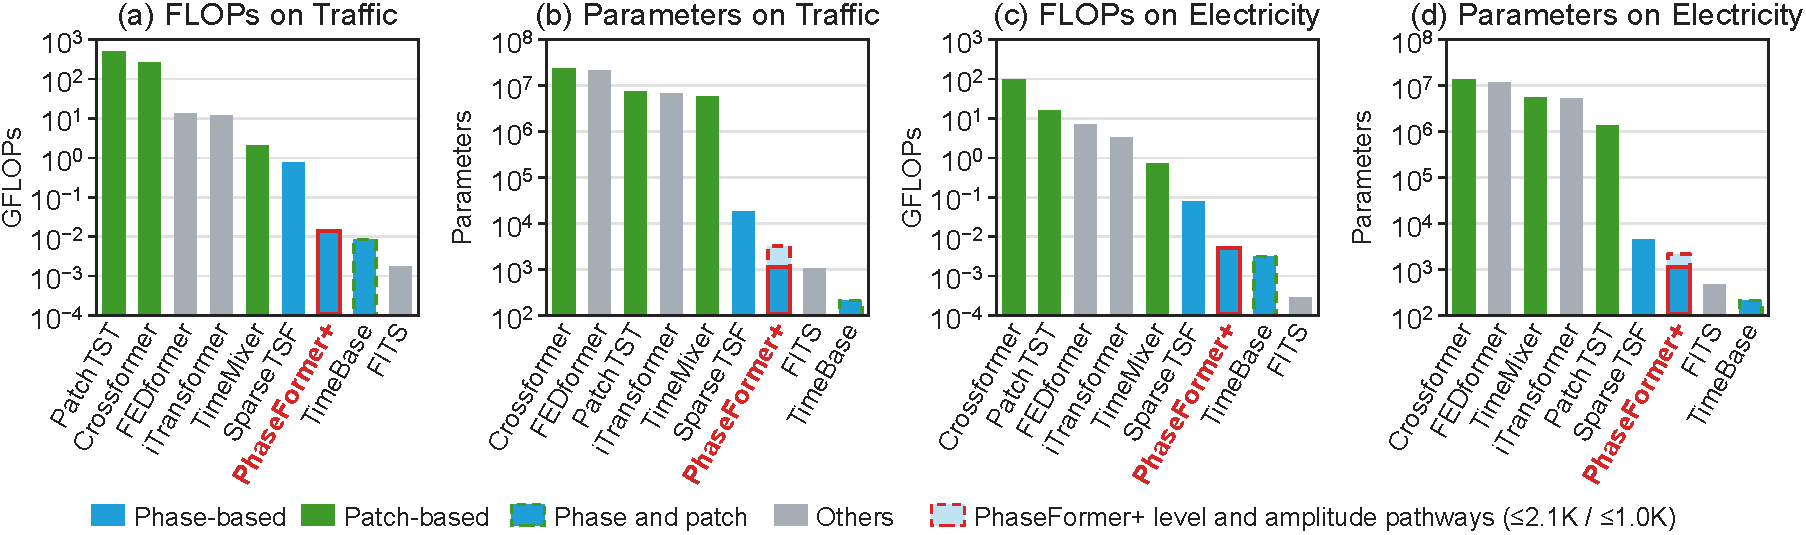
\includegraphics[width=\textwidth]{figures/efficiency_bars.pdf}
    \caption{\blue{\sysplus 与八个基线在 Traffic 和 Electricity 上的单次预测 FLOPs 与参数量，输入长度为 720 步，预测时域为 96（对数坐标）。基于相位的模型为蓝色，基于分块的模型为绿色，结合分块与相位的 TimeBase 为带绿色虚线边框的蓝色，其余模型为灰色。\sysplus 的柱形显示其相位通路；虚线部分加上其水平与振幅通路的参数量，在 Traffic 上至多约 2.1K，在 Electricity 上至多约 1.0K，这部分通路增加的 FLOPs 不足 0.25\%（第\ref{sec:exp_efficiency}节）。}}
    \label{fig:flops_params_visualization}
\end{figure*}

\subsection{\blue{效率}}
\label{sec:exp_efficiency}

我们评估所有模型的计算开销，详细结果见\blue{电子补充材料}。
\figref{fig:flops_params_visualization} 展示了\blue{\sysplus 与八个基线}在 Electricity 和 Traffic \blue{数据集}上的 FLOPs 与参数量。
总体而言，基于相位的模型开销低于基于分块的模型。
在 Traffic 数据集上，\blue{\sysplus 的相位通路}相较 PatchTST 和 Crossformer 将 FLOPs 降低约 99.99\%\blue{，参数量仅约 1.2K}。
这源于相位标记的\blue{低维性}（\secref{sec:mot_stability}）\blue{，使一个小的潜空间和少量路由器即可承载它们。在轻量模型中，\sysplus 在所有数据集上的 MSE 均低于 TimeBase 和 SparseTSF，并在七个数据集中的六个上低于 FITS（第\ref{sec:exp_results}节）。}
\blue{水平与振幅通路保持了这一效率特征。在主表配置的全部 28 个设置中，它们增加的参数量介于 119 到 679 之间。融合门控在共享时共增加两个参数，否则每通道增加两个（Traffic 上为 1{,}724）；它们是唯一规模随传感器数量增长的部分。计入它们后，水平与振幅通路至多增加约 2.1K 参数，最大增量出现在 Traffic 上（第\ref{sec:complexity}节与附录\ref{app:la_config}）。在单块 A800 GPU 上实测（fp32，批大小 32，$L{=}720$），它们使 Traffic 和 Electricity 上相位通路的 FLOPs 增加 $0.09\%$ 到 $0.23\%$：它们的运算——门控、融合、水平标记的周期均值以及两个秩至多为三的映射——相较路由层可以忽略不计。

电子补充材料将 CycleNet 加入对比，后者在 Electricity 上取得了低于 \sysplus 的数据集平均值（补充材料的分时域表中为 0.157，而表\ref{tab:main_results} 中为 0.159）。CycleNet 为每个通道存储一个学习到的周期，在 Electricity 上携带 472K 参数，在 Traffic 上携带 563K 参数，比 \sysplus 高出两个数量级，且这一开销随通道数量增长；\sysplus 则用一条共享通路从自身的相位标记中读取每个通道的形状（逐模型参数量与 FLOPs 对比见电子补充材料）。结合精度结果来看，\sysplus 在七个基准数据集中的六个上取得最佳平均 MSE，同时比 Transformer 基线便宜若干数量级。}

\subsection{\blue{相位通路分析}}
\label{sec:exp_ablation}

\blue{相位通路是三条通路中最大的一条，也是第\ref{sec:exp_ladder}节标记消融的基础。我们单独分析它，即不含水平与振幅通路的情形：其路由器、路由层、相位长度与注意力模式。}

\subsubsection{\blue{路由器数量与跨相位路由}}

\fakeparagraph{改变路由器数量}
我们系统地评估不同路由器数量 $M$ 对模型性能的影响，结果汇总于 \figref{fig:router_number_visualization}。
实验表明，在三个数据集上，模型的预测误差随路由器数量 $M$ 的增加总体呈下降趋势，最终趋于稳定或略有回升。
最佳性能通常在 $M \in \{4,8\}$ 时取得，\blue{远少于相位标记的数量（Electricity 和 Traffic 上为 24）}。
这一观察表明，相位标记张成本质上低维的空间，因此少量路由器便足以有效捕获并表示其底层结构\blue{，这与洞察 2（第\ref{sec:mot_stability}节）一致——根据该洞察，前两个主成分即可解释 Traffic 上相位标记的大部分方差}。
更详细的结果见\blue{电子补充材料}。

\begin{figure*}[t]
    \centering
    % 子图1
    \begin{subfigure}{0.32\textwidth}
        \centering
        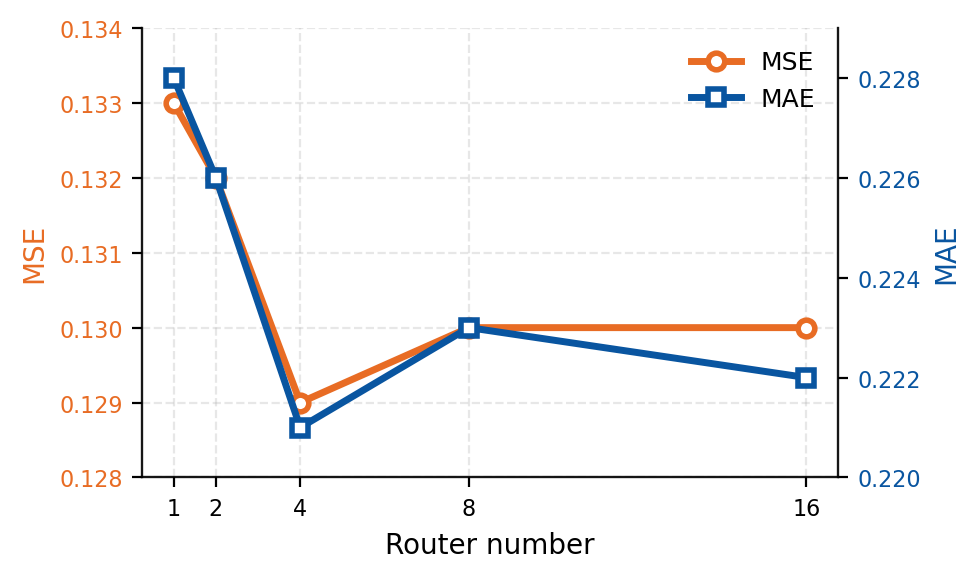
\includegraphics[width=\linewidth]{figures/router_number_effect_electricity_lines.png}
        \caption{Electricity}
        \label{fig:electricity}
    \end{subfigure}
    % 子图2
    \begin{subfigure}{0.32\textwidth}
        \centering
        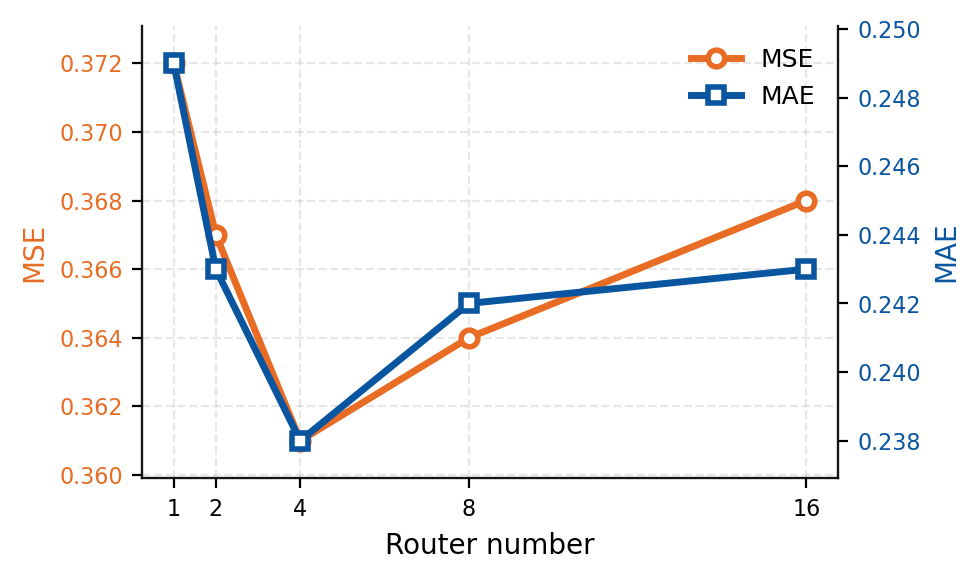
\includegraphics[width=\linewidth]{figures/router_number_effect_traffic_lines.png}
        \caption{Traffic}
        \label{fig:traffic}
    \end{subfigure}
    % 子图3
    \begin{subfigure}{0.32\textwidth}
        \centering
        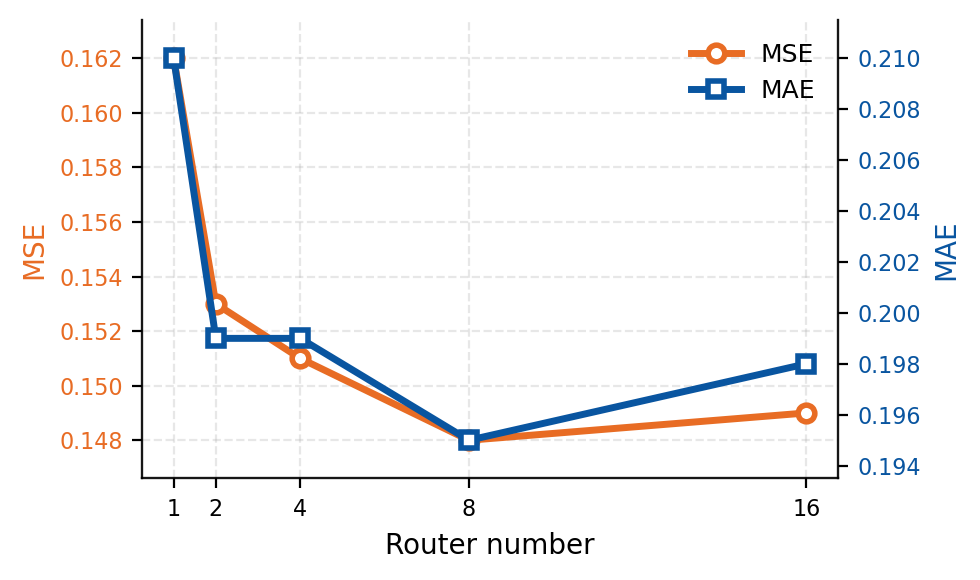
\includegraphics[width=\linewidth]{figures/router_number_effect_weather_lines.png}
        \caption{Weather}
        \label{fig:Weather}
    \end{subfigure}

    \caption{在三个数据集上改变路由器数量 $M$ 对预测性能的影响。}
    \label{fig:router_number_visualization}
\end{figure*}

\begin{table*}[t]
\centering
\caption{\blue{相位通路跨相位路由层的消融。}每个单元格报告 MSE、MAE 和 FLOPs。所有指标均为越低越好。FLOPs 以百万（MFLOPs）为单位报告。最好结果以\best{粗体}标出，次好结果以\second{下划线}标出。}
\label{tab:ablation_phase}
\footnotesize
\begin{tabular}{c|ccc|ccc|ccc|ccc}
\hline
\multirow{2}{*}{数据集}
& \multicolumn{3}{c|}{\textbf{路由}}
& \multicolumn{3}{c|}{\textbf{采用全注意力}}
& \multicolumn{3}{c|}{\textbf{采用线性混合}}
& \multicolumn{3}{c}{\textbf{去除路由}} \\
\cline{2-13}
& MSE & MAE & FLOPs
& MSE & MAE & FLOPs
& MSE & MAE & FLOPs
& MSE & MAE & FLOPs \\
\hline
Weather
& \best{0.1503} & \best{0.1971} & 3.119
& \second{0.1527} & \second{0.2005} & 3.202
& 0.1700 & 0.2226 & \second{0.920}
& 0.1907 & 0.2406 & \best{0.783} \\
\hline
Electricity
& \best{0.1290} & \best{0.2209} & 42.213
& \second{0.1295} & \second{0.2217} & 48.951
& 0.1403 & 0.2334 & \second{14.068}
& 0.1423 & 0.2365 & \best{11.972 } \\
\hline
Traffic
& \best{0.3721} & \best{0.2475} & 113.356
& \second{0.3791} & \second{0.2513} & 131.452
& 0.3842 & 0.2532 & \second{37.776}
& 0.3892 & 0.2584 & \best{32.149}  \\
\hline
\end{tabular}
\end{table*}

\fakeparagraph{跨相位路由的有效性}
为评估跨相位路由层的贡献，我们比较\blue{相位通路}的四个变体：
\textbf{路由}，采用跨相位路由层；
\textbf{采用全注意力}，用完整注意力机制替换跨相位路由层；
\textbf{采用线性混合}，用线性层替换跨相位路由层；
以及 \textbf{去除路由}，直接将每个相位投影到其自身的未来。
其余实验设置在这些变体之间保持完全一致。

如 \tabref{tab:ablation_phase} 所总结，\blue{路由}一致优于 \textbf{采用线性混合} 和 \textbf{去除路由}，表明显式的跨相位路由对建模周期性动态至关重要。此外，\blue{路由}不仅\blue{计算量}更小，预测误差也低于 \textbf{采用全注意力}，说明路由层兼具高效与有效。我们将这些增益归因于在低维相位标记空间中运算，该空间集中了信息丰富的交互并降低了开销。

\revised{
\subsubsection{对相位长度的敏感性}
\label{sec:phase_length}

\begin{table}[t]
\centering
\begin{tabular}{ccc}
\hline
\textbf{相位长度} & \textbf{MSE} & \textbf{MAE} \\
\hline
24 & 0.3619 & 0.2384 \\
12 & 0.3960 & 0.2765 \\
8  & 0.4032 & 0.2801 \\
28 & 0.4063 & 0.2753 \\
21 & 0.4184 & 0.2970 \\
\hline
\end{tabular}
\caption{Traffic 数据集上不同相位长度下预测性能的比较（\blue{$L=720$，$H=96$}）。}
\label{tab:phase_length}
\end{table}
\blue{\sysplus} 通过频域分析自动确定相位长度（见\blue{电子补充材料}），直接从数据中提取显著的周期成分。
为评估其对相位长度的敏感性，我们在 Traffic 数据集上开展实验。其频谱包含若干清晰的周期成分（见 \figref{fig:spectrum_traffic}）。我们基于谱幅值选出前五个候选相位长度，并运行\blue{相位通路}进行预测。结果如 \tabref{tab:phase_length} 所示。

\begin{figure}[t]
    \centering
    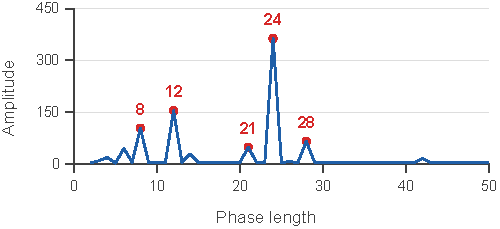
\includegraphics[width=\linewidth]{figures/spectrum_traffic.pdf}
    \caption{在 Traffic 数据集上计算的频谱。前五个相位长度为 24、12、8、28、21。}
    \label{fig:spectrum_traffic}
\end{figure}

实验表明，相位长度为 24 时模型表现最佳，对应主导谱成分。\blue{五个候选的 MSE 恰好按其谱幅值的顺序递增（\figref{fig:spectrum_traffic}），因此最强的谱成分也是最准确的相位长度。}
这些发现表明，\blue{相位通路}有效捕获了数据集的主要周期结构。
}

\subsubsection{案例分析}
\label{sec:exp_case}
我们从 Traffic 数据集中选取一个样本，包含长度为 720 的输入序列和长度为 96 的输出序列（共 816 个时间步）。
将输入序列送入\blue{相位通路}，我们记录第一个跨相位路由层在聚合（Phase$\rightarrow$Router）与分发（Router$\rightarrow$Phase）两个阶段的注意力权重矩阵。
如 \figref{fig:sender} 与 \figref{fig:receiver} 所示，两种注意力模式都呈现清晰的局部相似性：相邻相位往往被分配到相同的路由器，并从相似的路由器接收注意力。
这表明路由机制捕获了时间上连贯的相位关系。
同时，注意力权重显示某些相位具有相似的注意力模式。
为进一步分析，我们聚焦三个具有不同注意力模式的相位，并在 \figref{fig:traffic_data_visualization} 中将其\blue{可视化}。
这些相位表现出不同的时间行为：相位 5 在较长时域上保持相对稳定，而相位 9 和相位 1 都呈现明显的 7 天周期性，但趋势相反。
这些相位标记的不同模式表明，路由器结构不仅能区分相位标记，还能有效建模其\blue{每周模式与漂移}。
\blue{总的来说，这些分析说明了相位通路为何可以很小：相位标记是低维的，少量路由器即已足够；路由比完整注意力和无交换都更准确，且 FLOPs 至多比完整注意力少 14\%；主导周期也是最准确的相位长度。还有一点预示了标记消融：路由器曲线在少量路由器处便趋于平缓，因此相位通路中新增的容量不再带来收益，而仅有 105 个参数的水平通路仍能将 Weather 上的 MSE 改善 2.7\%（第\ref{sec:exp_ladder}节）。}


\begin{figure*}[t]
  \centering
  \begin{subfigure}{0.24\linewidth}
    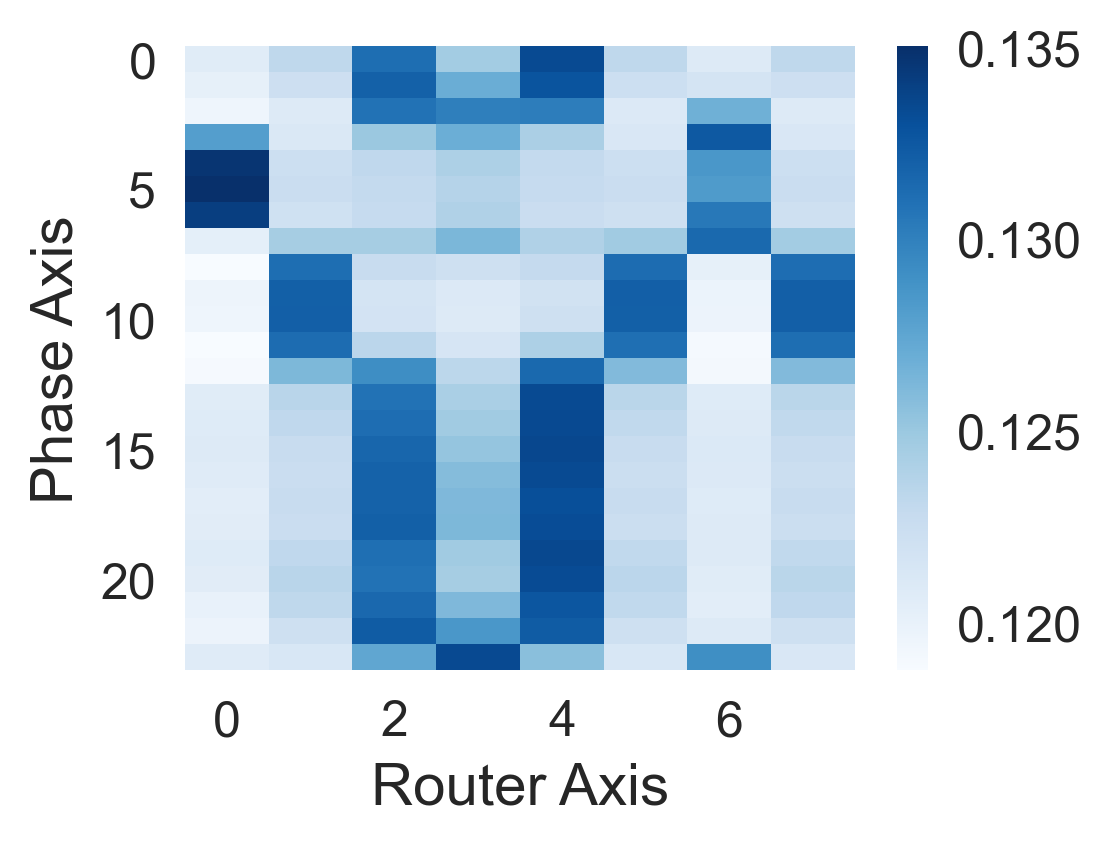
\includegraphics[width=\linewidth]{figures/attention_layer_0_sender_var4.png}
    \caption{聚合权重}
    \label{fig:sender}
  \end{subfigure}%
  \hfill
  \begin{subfigure}{0.24\linewidth}
    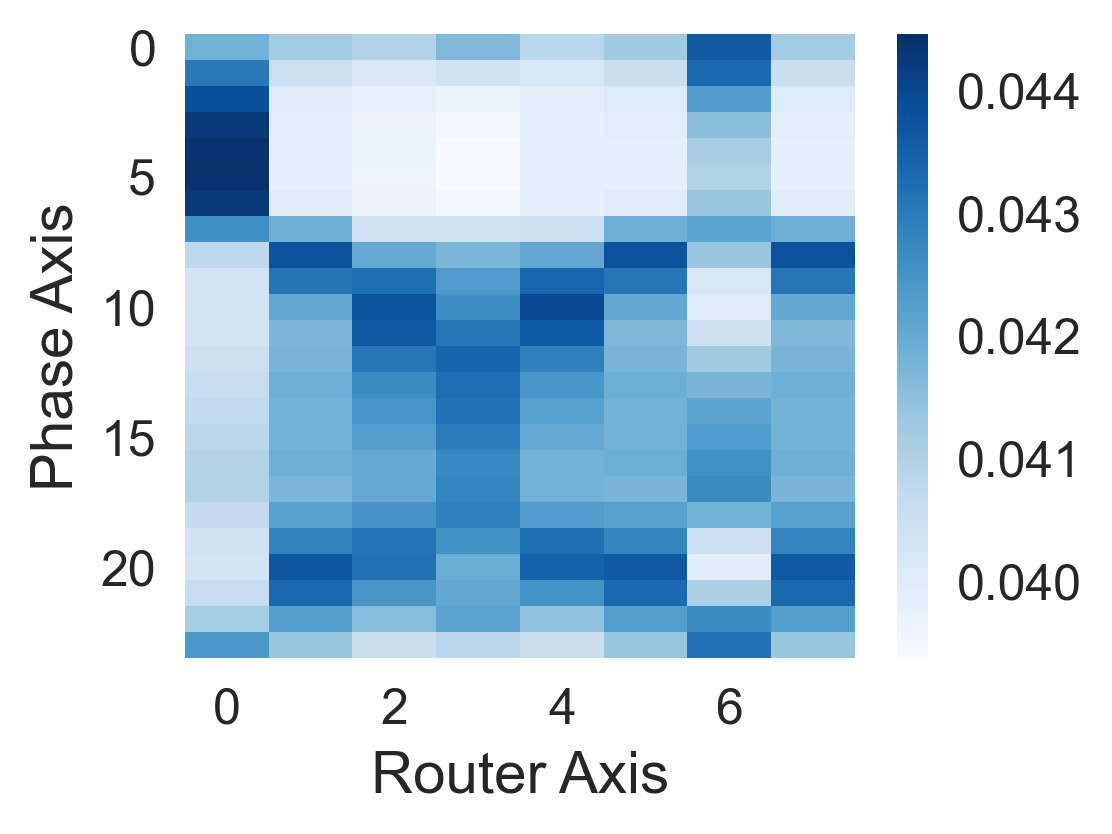
\includegraphics[width=\linewidth]{figures/attention_layer_0_receiver_var4.png}
    \caption{分发权重}
    \label{fig:receiver}
  \end{subfigure}
  \hfill
  \begin{subfigure}{0.48\linewidth}
    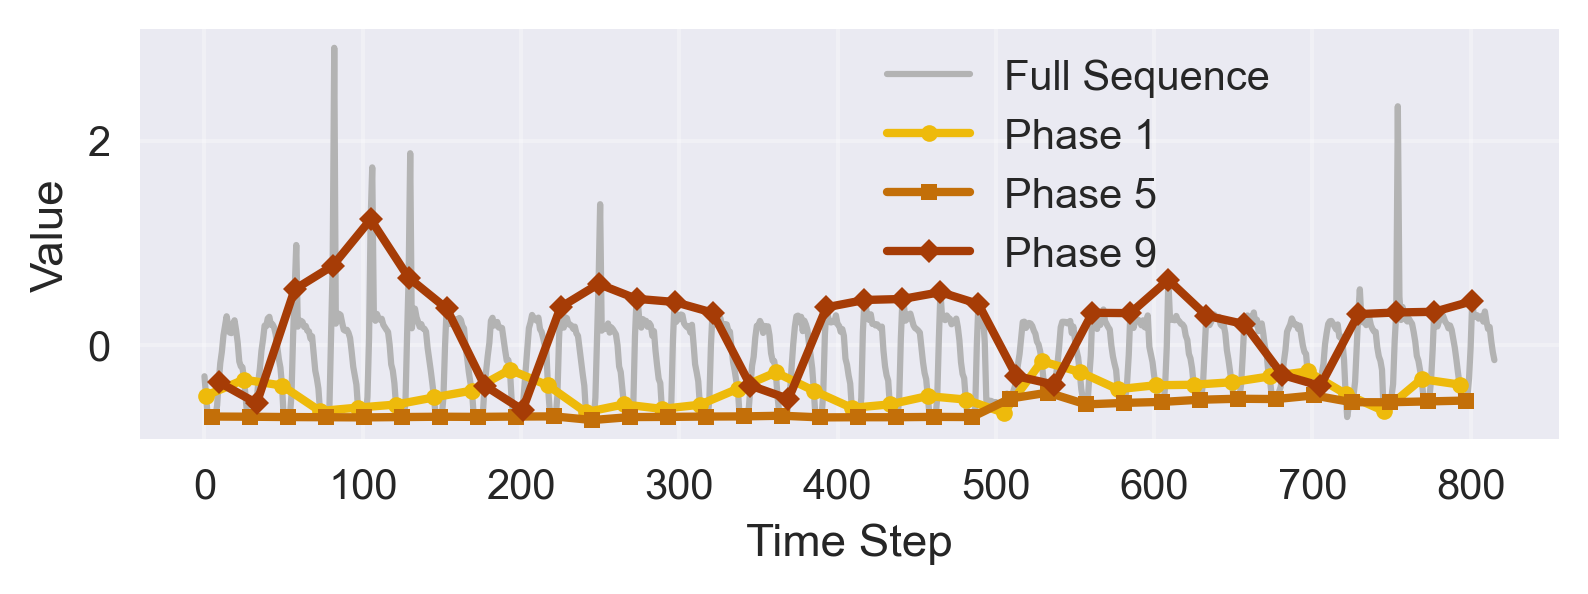
\includegraphics[width=\linewidth]{figures/sequence_with_phase_curves_sample_0_feature_0.png}
    \caption{三个选定相位标记的可视化}
    \label{fig:traffic_data_visualization}
  \end{subfigure}%
  \caption{Traffic 数据集一个样本的案例分析。
  (a) 相位到路由器聚合阶段的注意力权重矩阵。
  (b) 路由器到相位分发阶段的注意力权重矩阵。
  两个矩阵都刻画了 8 个路由器与 24 个输入相位之间的关联。
  (c) 三个代表性相位（1、5 和 9）的可视化，每个相位都对应一种与路由器交互的独特注意力模式。}
  \label{fig:case_study_wrap_all}
\end{figure*}

\blue{
\subsection{每个标记都不可或缺}
\label{sec:exp_ladder}

\begin{table*}[t]
\blue{
\centering
\caption{标记消融：\sysplus 逐个添加标记构建。测试 MSE/MAE 为四个预测时域与三个种子上的平均值，所有变体在同一协议下训练（协议配置，第\ref{sec:ext_setup}节）。仅相位：仅相位变体；相位 + 水平：相位–水平变体；\sysplus（关闭振幅）：关闭振幅通路后的训练好的 \sysplus。粗体：前三列中的最佳值。正文中的相对差异基于未取整的平均值计算。}
\label{tab:ladder}
\footnotesize
\setlength{\tabcolsep}{6pt}
\begin{tabular}{lcccccccc}
\toprule
数据集 & \multicolumn{2}{c}{仅相位} & \multicolumn{2}{c}{相位 + 水平} & \multicolumn{2}{c}{\sysplus} & \multicolumn{2}{c}{\begin{tabular}[c]{@{}c@{}}\sysplus\\（关闭振幅）\end{tabular}} \\
\cmidrule(lr){2-3}\cmidrule(lr){4-5}\cmidrule(lr){6-7}\cmidrule(lr){8-9}
 & MSE & MAE & MSE & MAE & MSE & MAE & MSE & MAE \\
\midrule
ETTh1 & 0.408 & \textbf{0.419} & 0.412 & 0.425 & \textbf{0.405} & 0.421 & 0.414 & 0.429 \\
ETTh2 & 0.354 & 0.396 & \textbf{0.347} & \textbf{0.393} & 0.348 & \textbf{0.393} & 0.352 & 0.396 \\
ETTm1 & \textbf{0.352} & \textbf{0.377} & 0.354 & 0.380 & 0.353 & 0.380 & 0.355 & 0.381 \\
ETTm2 & 0.258 & 0.319 & \textbf{0.253} & \textbf{0.315} & \textbf{0.253} & \textbf{0.315} & 0.257 & 0.318 \\
Weather & 0.227 & 0.262 & 0.221 & \textbf{0.257} & \textbf{0.220} & \textbf{0.257} & 0.220 & 0.257 \\
Electricity & 0.161 & \textbf{0.251} & \textbf{0.160} & \textbf{0.251} & \textbf{0.160} & \textbf{0.251} & 0.162 & 0.254 \\
Traffic & \textbf{0.392} & \textbf{0.248} & 0.395 & 0.251 & 0.393 & 0.252 & 0.400 & 0.256 \\
\bottomrule
\end{tabular}
}
\end{table*}

表\ref{tab:ladder} 在协议配置下、全部 28 个设置、三个种子上逐个添加标记构建 \sysplus：先是仅相位变体（第\ref{sec:ext_setup}节），然后是水平标记，再是振幅标记；其最后一列为在训练好的 \sysplus 上关闭振幅通路。在同一协议下，\sysplus 在七个数据集平均值中的五个上优于其仅相位变体，幅度介于 0.4\% 到 3.3\% 之间；在 ETTm1 和 Traffic 上与其相差不超过 0.3\%，参数开销约为 130--170（不含融合门控）。包络同时预示了这一结果的两个方面。四个最大的增益恰好落在四个包络生效的数据集上：Weather、ETTm2 和 ETTh2 上的水平包络，以及 ETTh1 上的振幅包络（表\ref{tab:envelope}）。在 ETTm1、Electricity 和 Traffic 上，落在任一包络之外的测试窗口都不超过 3.5\%，误差变化至多 0.4\%，正如理论所预测。在主表配置下，\sysplus 在 ETTh2、ETTm2 和 Weather 的每个预测时域上都优于仅相位变体，且优势超过一个种子标准差（表\ref{tab:la_full}）。

\fakeparagraph{水平标记}
水平标记恰好在水平包络生效之处取得增益，无论在仅相位变体上还是在 \sysplus 上皆如此（第\ref{sec:exp_envelopes}节）。在 ETTh2、ETTm2 和 Weather 上，分别有 7.8\% 到 9.7\% 的测试窗口落在仅相位变体的包络之外，12\% 到 21\% 落在 \sysplus 的包络之外，水平标记将 MSE 分别改善 2.0\%、1.8\% 和 2.7\%；在其余四个数据集上（落在包络之外的窗口至多 3.5\%），它对误差的改变至多 1.0\%。

\fakeparagraph{振幅标记}
振幅标记补充了水平标记所无法提供的能力。ETTh1 是唯一一个振幅包络生效而水平包络几乎不生效的数据集（窗口占比 14.8\% 对 2.5\%，表\ref{tab:envelope}）；在此，仅添加水平标记会使误差增加 1.0\%，振幅标记带来了恢复，\sysplus 最终比仅相位变体低 0.7\%。在训练好的模型上关闭振幅通路会消除全部增益（0.414 对 0.405）。在全部 28 个设置中，振幅通路在 27 个设置上改善了其所属模型。

\fakeparagraph{弱耦合与强耦合}
在耦合最弱的两个基准数据集 ETTh2 和 ETTm2 上（第\ref{sec:mot_changes}节），增益由水平标记贡献，而振幅通路在 \sysplus 内部仍在发挥作用：关闭它会使 MSE 从 0.348 升至 0.352、从 0.253 升至 0.257。在耦合如此弱的情况下，ETTh2 上超出振幅包络的 31.8\% 窗口，其超出量来自窗口自身的形状 $\Omega_0$，而非水平。在耦合最强的基准数据集 Traffic 上，尽管没有窗口超出包络，振幅通路仍改善了其所属模型（0.393 对关闭时的 0.400）；这一增益将 $q$ 的静态逐通道修正（第\ref{sec:exp_mechanism}节）与依赖水平的部分结合起来，下文的分层分析将其揭示出来。

\fakeparagraph{增益出现之处}
如果振幅通路承载的是跟随水平的振幅，那么 \sysplus 相对其相位–水平变体的逐窗口增益应随水平需求增长。按 $|\Lambda|$ 的五分位数对逐窗口测试增益分层的结果支持这一点。在全部 28 个设置中，最高五分位的 MSE 降幅比最低五分位多 $0.002$；在 \sysplus 平均而言有所改善的大多数设置上，最高五分位的平均增益超过最低五分位，其中最强的设置从低到高逐层上升（Traffic-$96$：各五分位从 $+0.0002$ 到 $+0.0033$；ETTh1-$192$：$-0.0033$ 到 $+0.0052$；Weather-$96$：$-0.0031$ 到 $+0.0080$）。因此，振幅通路在水平变化最大的窗口上增益最大。
}

\blue{
\subsection{验证统一视角}
\label{sec:exp_theory}

第\ref{sec:theory}节分三步展开论证，每一步都可以在训练好的模型上检验。必要性：包络在每个训练好的模型上都成立，并在数据的需求超出它们之处生效；此时水平通路接管水平，而振幅通路不改变任何周期均值，因此它无法替代水平通路（第\ref{sec:exp_envelopes}节与第\ref{sec:exp_mechanism}节）。形式：振幅通路的增益随数据中由水平驱动的振幅而增长，并读取水平（第\ref{sec:exp_mechanism}节）。充分性：三个固定轮廓、105 个参数，与可学习解码器相比几乎没有损失（第\ref{sec:exp_capacity}节）。

\subsubsection{包络与分工}
\label{sec:exp_envelopes}

定理\ref{thm:level_envelope}与定理\ref{thm:amplitude}的常数是权重的函数，因此可以从每个训练好的模型中读出，而需求是数据的函数。表\ref{tab:envelope} 针对训练好的 \sysplus 模型（在四个预测时域上取平均）报告了这两组量，以及每个测试窗口的水平需求 $\Lambda$ 与振幅需求 $\Omega$。

\begin{table}[t]
\blue{
\centering
\caption{训练好的 \sysplus 模型相位通路的包络（协议配置；预测时域上的平均值；振幅通路已关闭）。$C_1$、$B_\varphi$：水平包络与振幅包络的半宽，从权重中读出；$g_s$：形状门控；$\mathcal I_\varphi$ 之外：水平需求 $\Lambda$ 落在水平包络之外的测试窗口占比；下界/MSE：误差下界~\equref{eq:level_floor} 占测试 MSE 的比例；$\Omega$ 超包络：振幅需求超过 $(1-g_s)B_\varphi$ 的窗口占比。}
\label{tab:envelope}
\footnotesize
\setlength{\tabcolsep}{2.6pt}
\begin{tabular}{lcccccc}
\toprule
数据集 & $C_1$ & $B_\varphi$ & $g_s$ & $\mathcal I_\varphi$ 之外 & 下界/MSE & $\Omega$ 超包络 \\
\midrule
ETTh1 & 1.35 & 1.37 & 0.23 & 2.5\% & 0.08\% & 14.8\% \\
ETTh2 & 1.07 & 1.08 & 0.25 & 19.4\% & 5.0\% & 31.8\% \\
ETTm1 & 1.86 & 1.99 & 0.35 & 3.5\% & 0.27\% & 2.2\% \\
ETTm2 & 1.39 & 1.47 & 0.26 & 12.5\% & 10.6\% & 5.7\% \\
Weather & 1.41 & 1.61 & 0.68 & 20.7\% & 11.6\% & 27.6\% \\
Electricity & 3.80 & 3.81 & 0.27 & 0.1\% & 0.5\% & 0.2\% \\
Traffic & 5.23 & 5.25 & 0.21 & 0.0\% & 0.0\% & 0.0\% \\
\bottomrule
\end{tabular}
}
\end{table}

\fakeparagraph{包络成立}水平包络严格按所述成立：在全部 84 个训练好的模型（28 个设置、三个种子）中，相位预测的实测水平从未离开 $\mathcal I_\varphi$，$|\lev(F)-c_0|/C_1$ 的最大观测值为 $0.74$，因此下文给出的下界是保守的。

\fakeparagraph{包络在理论预测之处生效}在包络生效之处，其生效方式与理论预测一致。在 ETTh2、Weather 和 ETTm2 上，有 12\% 到 21\% 的测试窗口的水平需求落在区间之外，下界占测试 MSE 的 5.0\% 到 11.6\%；并且在 ETTh2 和 Weather 上，包络外窗口的占比与区间的收紧程度都随预测时域增长（ETTh2：在 $H=96$ 到 $H=720$ 之间，$C_1$ 从 1.27 降到 0.85，包络外占比从 15\% 升到 27\%；Weather：从 1.86 降到 0.96，从 10\% 升到 34\%）。在两个传感器网络数据集上，训练好的模型的相位通路形成了几乎没有任何测试窗口能越出的宽包络。它们的半宽（$C_1$ 介于 3.8 与 5.2 之间）低于一致跟踪最后一个周期水平所需的 5.39（第\ref{sec:theory_level}节），但测试窗口的水平需求更小，下界至多占测试 MSE 的 0.5\%。因此，包络在这些数据集上几乎没有给相位通路带来损失，添加水平与振幅标记在这两个数据集上对误差的改变不足 1\%（第\ref{sec:exp_ladder}节）。

\fakeparagraph{分工遵循包络}水平门控在每个数据集上取得相近的份额（$g_\ell$ 平均在 0.20 到 0.26 之间），但水平通路如何使用其份额取决于包络是否生效：在包络较窄（$C_1\le1.86$）的四个 ETT 数据集上，水平通路的水平预测与窗口水平需求的相关系数在 $0.40$ 到 $0.44$ 之间；而在包络较宽的 Electricity 和 Traffic 上，分别为 $0.03$ 和 $-0.01$。水平通路在相位通路无法跟踪水平之处跟踪水平，正如定理\ref{thm:complement}(b) 所预测。

以同样方式考察 84 个训练好的仅相位变体可以看出，这一模式是数据的属性，在没有水平与振幅标记时同样存在。它们的预测水平同样从未离开包络（最大观测利用率为 $0.87$），且水平包络在同样的三个数据集上生效：在 ETTh2、ETTm2 和 Weather 上，有 7.8\% 到 9.7\% 的测试窗口落在包络之外，下界占测试 MSE 的 1.7\% 到 4.1\%，而在其余四个数据集上分别至多只有 3.5\% 和 0.6\%。与水平通路共同训练时，\sysplus 的相位通路在这三个数据集上收窄了其包络（$C_1$ 从 1.72--2.16 之间降到 1.07--1.41 之间），在 ETTh1 和 ETTm1 上的变化不超过 0.1，并在两个传感器网络数据集上加宽了包络：在水平包络生效之处，它把水平留给水平通路，这正是定理\ref{thm:complement}(b) 的分工。

\subsubsection{振幅通路}
\label{sec:exp_mechanism}

\fakeparagraph{合成乘性序列}
我们首先在真值已知的场景下检验定理\ref{thm:amplitude}。我们按 \equref{eq:mult_model} 生成具有随机游走水平、正弦日轮廓和耦合 $\alpha\in\{0,0.25,0.5\}$ 的七通道序列，并从相同初始化训练 \sysplus 及其相位–水平变体（两个种子、30 轮）。无耦合（$\alpha=0$）时，振幅通路无事可承，两个模型难分伯仲：\sysplus 的验证 MSE 变化为 $-0.28\%$。有耦合时，\sysplus 在 $\alpha=0.25$ 下将验证 MSE 降低 $3.3\%$，在 $\alpha=0.5$ 下降低 $4.8\%$，且对两个种子均是如此。增益恰好在数据包含跟随水平的振幅时出现，并随耦合增强而增长，正如定理\ref{thm:amplitude}(b) 中需求的形式与命题\ref{prop:modulation}(b) 的构造所蕴含的那样。

\fakeparagraph{周期均值不变性}
命题\ref{prop:modulation}(a) 是精确的恒等式，因此我们在每个训练好的 \sysplus 上对其进行验证。在双精度下开关振幅通路，对相位预测的每个未来周期均值的绝对改变至多为 $8.9\times10^{-16}$，而容差为相对于预测尺度的 $7\times10^{-9}$，而对单个相位预测的改变最多可达 $1.8$ 个窗口标准差。全部 84 个训练好的模型（28 个设置、三个种子）均通过验证。

\fakeparagraph{振幅通路读取水平}
命题\ref{prop:modulation}(b) 预测振幅通路会读取水平：其构造 $q=\alpha_w\hat\Lambda\,\one_d$（其中 $\hat\Lambda$ 为水平通路的水平预测）以因子 $1+\alpha_w\hat\Lambda$ 缩放相位振幅。训练好的模型证实了这一点，在 $H=96$ 时最为清晰；在读取水平较弱之处，振幅通路充当静态的逐通道振幅修正，这由 $q$ 的均匀分量提供（第\ref{sec:theory_amplitude}节）。我们逐通道计算 $q$ 沿 $\one_d$ 方向的分量与窗口水平需求 $\Lambda$ 的相关系数；合并通道会把 $q$ 中由水平驱动的部分与其依赖通道的静态尺度混在一起。在 $H=96$ 时，逐通道平均相关系数在 Weather 上为 $0.46$（86\% 的通道）、在 Electricity 上为 $0.30$（全部 166 个显著通道同号）、在 ETTh2 上为 $0.54$（每个通道都超过 $0.3$）；在七个数据集上按预测时域平均后介于 $0.12$ 与 $0.37$ 之间。学习到的耦合符号在每个设置内保持一致——Weather-$96$ 的显著通道与 Electricity-$96$ 的符号相反——这是构造所允许的，因为 $\alpha_w$ 是学习得到的。

在 ETTm1-$96$ 和 ETTm2-$96$ 上相关系数较低（$0.27$ 和 $0.02$）：在这两个设置上，振幅通路主要充当静态修正。另外两个观察也与构造一致：$q$ 与振幅需求 $\Omega$ 本身仅有弱相关（各处逐通道平均相关系数均低于 $0.20$），因此它跟随的是水平而非振幅；$q$ 的静态部分是一个逐通道振幅修正，其移除可以解释表\ref{tab:ladder} 中关闭振幅列在七个数据集中六个上的退化。

\subsubsection{水平通路的容量}
\label{sec:exp_capacity}

定理\ref{thm:complement}(a) 预测，在标准季节模型下，相位通路无法企及的水平通过少数固定时域轮廓进入，因此轮廓预先固定的水平通路与学习这些轮廓的水平通路相比应当毫无损失。第\ref{sec:ext_setup}节的选择实验提供了直接检验。在相同秩下，三种解码器的参数量差异悬殊：可学习解码器分别有 477 和 657 个参数，是固定轮廓 105 个参数的四到七倍。然而它们的按设置归一化的验证误差——在七个数据集与两种门控变体上平均——仅相差 0.13\%：相对于每个设置的最佳变体，基于 90 个池化值的解码器为 1.0102，基于 30 个池化值的解码器为 1.0107，固定轮廓为 1.0115。固定轮廓落在与最佳解码器相差 0.5\% 的平局范围内，并因其最小而入选。因此，限制在偏移、倾斜与曲率轮廓张成空间中的水平通路，与能学习任意时域轮廓的水平通路相比几乎没有损失，正如定理\ref{thm:complement}(a) 所预测；这三个轮廓已经足够：即便在主表配置中，28 个设置中也有 24 个保留它们（附录\ref{app:la_config}）。

}

\blue{
\subsection{总结}
\label{sec:exp_summary}

实验回答了本节的三个问题。其一，\sysplus 既准确又小巧：它在七个基准数据集中的六个上取得最佳平均 MSE，并在全部七个上排名第一或第二。在最大的基准数据集 Traffic 上，其相位通路仅需约 1.2K 参数，即可将 PatchTST 和 Crossformer 的 FLOPs 降低约 99.99\%，而水平与振幅通路至多增加约 2.1K 参数。其二，每个部分都不可或缺：在相位通路中，跨相位路由比完整注意力和无交换都更准确，且只需少量路由器；在统一协议下逐个添加标记构建时，\sysplus 恰在包络预测之处获得增益，其四个最大的增益正落在四个包络生效的数据集上。其三，训练好的模型的表现与统一视角的预测一致：水平包络在每个模型上都成立，并且恰好在水平标记增益最大的三个数据集上生效；振幅通路精确保持每个周期均值并读取水平；三个固定轮廓足以支撑水平通路。因此，预测周期性传感器数据流并不需要当前模型那样的复杂度：有了覆盖形状、水平与振幅的标记，一个只有几千个参数的模型便已足够。
}

\section{\blue{结论}}
\label{sec:conclusion}

\blue{
预测模型正变得日益复杂，本文追问周期性传感器数据流是否需要这种复杂性。答案是否定的。周期序列的一个窗口携带三类信息——其各周期的形状、水平与振幅——它们构成一个低维结构：一个水平项加一个振幅缩放的形状，在七个基准数据集上捕获归一化窗口的 78\% 至 93\%。\sysplus 为每个部分赋予一个标记和一条小通路：相位标记——当每个周期以相同方式重塑时，它们停留在一个固定子空间中——通过一个带少量路由器与一个共享预测器的路由 Transformer 承载形状；水平标记即各周期均值，被映射到三个固定的预测时域轮廓上；振幅标记由水平计算，在可证明地保持每个未来周期均值不变的前提下缩放周期形状。统一的低维视角说明了三个标记为何缺一不可、每条通路为何取其形式：对固定权重，通过层归一化读取相位标记的预测模型，将其预测水平与振幅限制在两个任何附加深度都无法消除的包络内，而包络之外只是少数几个轮廓系数和一个由水平驱动的因子。从训练后的模型读出的包络，恰好在水平与振幅标记收益最大之处约束生效。

\sysplus 以其相位通路约 1.2K 参数量、水平与振幅至多再加约 2.1K 参数量，在七个基准数据集中的六个上取得了相对八个基线的最佳平均 MSE；在最大的基准数据集 Traffic 上，它将 PatchTST 和 Crossformer 的 FLOPs 削减约 99.99\%。由于一个共享模型服务每个传感器，这些节省会在网络每个传感器上、每次更新时重复兑现；而振幅标记承载的水平–振幅耦合在 Traffic 与 Electricity 这两个传感器网络上最强。更广泛地说，这些结果表明，预测模型所需的容量取决于其标记留下多少纠缠：有了覆盖预测所需内容的标记，小模型便已足够。

\fakeparagraph{局限与未来工作}
\sysplus 是通道独立的：它通过并行与一个共享模型来利用传感器网络的规模，而将其标记与显式空间建模相结合是自然的下一步。我们结果中关于能力的部分，是在季节性随机游走及其乘性变体下的存在性结果；而包络对每个参数取值都成立，并在训练后的模型上被测量。分析假设单一主导周期，以及为整数个周期的预测时域；多个相互作用的周期与无明显周期的序列，以及通路之间依赖输入的门控，都留待未来工作。
}

\begin{acknowledgements}
本工作部分受到以下资助：国家自然科学基金（NSFC）（Grant Nos. 62425202, 62336003）、北京市自然科学基金（Z230001）、中央高校基本科研业务费 No. JK2024-03、滴滴合作研究计划、复杂与关键软件环境国家重点实验室（SKLCCSE）、虚拟现实技术与系统国家重点实验室（北京航空航天大学）开放课题计划（No.VRLAB2024A02）。
\end{acknowledgements}

\blue{
\section*{声明}

\fakeparagraph{基金资助}
资助来源见致谢。

\fakeparagraph{利益冲突}
作者声明不存在与本文内容相关的竞争性利益。

\fakeparagraph{先前发表}
本文是发表于 ICLR 2026 的会议论文~\citep{niu2026phaseformer}的扩展版本。两个版本之间的关系在第\ref{sec:intro}节末尾说明。

\fakeparagraph{数据可用性}
本研究使用的所有数据集均为公开可用的基准数据集；其来源见第\ref{sec:exp_main}节，其统计信息见电子补充材料。

\fakeparagraph{代码可用性}
{\sloppy \sysplus 的代码以及本文全部实验的脚本可在 \url{\codeurl} 获取。\par}

\fakeparagraph{大语言模型的使用}
本文使用大语言模型进行文字润色、语法问题识别与校对。
}


\bibliographystyle{spmpsci}
\bibliography{references}

\appendix
\blue{
\section{第\ref{sec:theory}节的证明}
\label{app:proofs}

全文中，$\tilde X\in\mathbb R^{K\times P}$ 表示折叠后的归一化窗口，其相位标记为 $\tilde x_p$、周期均值为 $\bar r$，并满足 $\one^\top\tilde x=0$、$\|\tilde x\|^2\le L$、$\one^\top\bar r=0$ 与 $\|\bar r\|^2\le K$。一个路由层（第\ref{subsec:phase-network}节）将标记 $h_1,\dots,h_P\in\mathbb R^d$ 映射为
\begin{equation*}
\begin{gathered}
	u_p=h_p+\pi_p,\quad
	\rho'_j=\operatorname{Attn}_s(\rho_j;u_{1:P}),\\
	m_p=\operatorname{Attn}_r(u_p;\rho'_{1:M}),
\end{gathered}
\end{equation*}
\begin{equation*}
o_p=\LN_1(u_p+m_p),\qquad h_p^+=\LN_2\big(o_p+\operatorname{MLP}(o_p)\big),
\end{equation*}
其中 $\rho_j$ 为路由器，$\pi_p$ 为位置嵌入，且
\begin{equation*}
\operatorname{Attn}(z;s_{1:n})=W_o\operatorname{concat}_{\text{heads}}\big(\sum_i\alpha_i(W_vs_i+c_v)\big)+c_o,
\end{equation*}
权重 $\alpha_i$ 为 $\langle W_qz+c_q,W_ks_i+c_k\rangle$ 在每个头内对 $i$ 的 softmax。第一层接收嵌入 $h^{(0)}_p=\LN_e(W_e\tilde x_p+b_e)$。在 $N_r$ 层的堆叠中，第 $l+1$ 层接收 $h^{(l)}_p+\LN'_l\big(W'_l(U_lh^{(l)}_p+c_{U,l})+c'_l\big)$，即上一层的输出加上对其投影 $U_lh^{(l)}_p+c_{U,l}\in\mathbb R^{\Pin}$ 的再嵌入，因此每层的最后一个运算都是 $\LN_2$。

\subsection{季节随机游走预测器}

对满足 $\one^\top b=1$ 且 $\|b\|\le1$ 的 $b\in\mathbb R^K$，\emph{水平自适应季节预测器}定义为
\begin{equation}
G_b(\tilde X)_p=\one_{K'}\Big[\tfrac1K\one_K^\top\tilde x_p+\big(b-\tfrac1K\one_K\big)^\top\bar r\Big],\qquad p=1,\dots,P .
\label{eq:gb}
\end{equation}
其水平为 $\lev(G_b)=b^\top\bar r$，因为 $\one^\top\bar r=0$。

\begin{lemma}[贝叶斯 预测]
\label{lem:bayes}
在 $\alpha=0$ 的模型~\equref{eq:mult_model}、高斯水平增量与噪声、以及季节轮廓和初始水平上的平坦先验下，采用局部水平模型在周期均值上的 Kalman 权重的 $G_b$ 是每个未来周期的后验均值预测。它是线性的，且满足 $G_b(aX+c\one\one^\top)=aG_b(X)+c\one\one^\top$，因此在 RevIN 坐标中预测、再反归一化即可在原始窗口上复现它。在稳态下，权重为 $b_k\approx\kappa(1-\kappa)^{K-k}$，其中 $\kappa=\tfrac12(-\tau+\sqrt{\tau^2+4\tau})$，$\tau=P\sigma_\eta^2/\sigma_e^2$。
\end{lemma}

\begin{proof}
对于高斯噪声，周期均值 $r_k=\tfrac1P\sum_pX_{kp}=\ell_k+\bar e_k$ 与相位偏差 $X_{kp}-r_k=s_p+(e_{kp}-\bar e_k)$ 相互独立，且偏差不涉及 $\ell$。偏差以后验均值 $\tfrac1K\sum_k(X_{kp}-r_k)$ 识别出 $s_p$。周期均值构成一个观测方差为 $\sigma_e^2/P$ 的局部水平模型，其在每个未来周期的后验均值即 Kalman 预测 $b^\top r$。将两个后验均值相加即得原始数据上的~\equref{eq:gb}。线性性是显然的，而 $(b-\tfrac1K\one)^\top\one=0$ 给出平移性质。 \qed
\end{proof}

\subsection{命题\ref{prop:capability}的证明}

\fakeparagraph{完整陈述} 考虑具有一个路由层、潜在宽度 $d\ge4$ 以及任意数量路由器和头的相位通路。
(a) 它对窗口的水平与尺度精确等变：当 $a>0$ 时 $F(ax+c\one)=aF(x)+c\one$。
(b) 周期水平的轨迹以共同平移的形式进入每个相位标记，而路由器注意力会将其输入的共同平移传递下去：发送方权重保持不变，每个路由器缓冲区平移同一向量（引理\ref{lem:shift}）。LayerNorm 只能近似保持共同平移，部分~(c) 通过一个大偏移来控制这一点。
(c) 对每个满足 $\one^\top b=1$ 且 $\|b\|\le1$ 的权重向量 $b$，存在参数 $\theta_c$（$c^2\ge5L$），其预测在所有归一化窗口上一致逼近 $G_b$，误差至多为 $\kappa_0L^{3/2}/c^2$，其中 $\kappa_0$ 为绝对常数。由引理\ref{lem:bayes}，相位通路因此可以把 $\alpha=0$ 的模型~\equref{eq:mult_model} 的 贝叶斯 预测逼近到任意精度。

\begin{lemma}[共同平移透传]
\label{lem:shift}
若路由层的每个输入标记都平移同一向量，即 $u_p\mapsto u_p+v$，则每个发送方权重保持不变，每个路由器缓冲区平移 $V_sv$（其中 $V_s=W^s_oW^s_v$），每个接收方输出平移 $V_rV_sv$ 加上接收方对未平移缓冲区重新加权产生的效应（其中 $V_r=W^r_oW^r_v$）。
\end{lemma}

\begin{proof}
路由器 $j$ 与标记 $p$ 的发送方得分在每个头中变化 $\langle W_q\rho_j+c_q,W_kv\rangle$，它与 $p$ 无关，故在关于 $p$ 的 softmax 中相消。缓冲区是 $W_v(u_p+v)+c_v$ 的凸组合再经 $W_o$ 作用，由此得到缓冲区的平移。接收方权重可能改变，但它们是凸组合，且每个缓冲区平移同一向量，因此输出平移 $V_rV_sv$，而重新加权只作用于未平移的缓冲区。 \qed
\end{proof}

\begin{lemma}[LayerNorm 的大偏移线性化]
\label{lem:ln_linear}
设 $e_0\perp\one_d$ 且 $\|e_0\|^2=d$，$w\perp\{\one_d,e_0\}$，$\gamma=\one$，$\beta=0$，$c>0$。则 $c\LN(ce_0+w)=(1-\eta)(ce_0+w)$，其中 $0\le\eta\le\rho^2/(2c^2)$，$\rho^2=\|w\|^2/d+\epsilon$。
\end{lemma}

\begin{proof}
由于 $J_d(ce_0+w)=ce_0+w$ 且 $\|ce_0+w\|^2/d=c^2+\|w\|^2/d$，故 LayerNorm 的尺度为 $c(1+\rho^2/c^2)^{1/2}$，而 $1-(1+t)^{-1/2}\le t/2$。 \qed
\end{proof}

\begin{proof}[命题\ref{prop:capability}的证明]
(a) RevIN 将 $ax+c\one$ 映射到同一个 $\tilde x$，反归一化恢复出 $a\sigma$ 与 $a\mu+c$。(b) 周期水平的轨迹 $\ell\in\mathbb R^K$ 为每个相位标记加上 $\ell$，从而为每个嵌入预激活加上 $W_e\ell$；引理\ref{lem:shift} 适用于路由层输入的任意共同平移。

(c) 选取正交的 $e_0,e_1,e_2\perp\one_d$ 且 $\|e_i\|^2=d$，由于 $d\ge4$ 这是可行的。设 $\alpha_1=\tfrac1K\one_K$，$\alpha_2=b-\tfrac1K\one_K$，$f_p=(\alpha_1-\alpha_2)^\top\tilde x_p$，$g_p=\alpha_2^\top\tilde x_p$。取 $W_e=e_1(\alpha_1-\alpha_2)^\top+e_2\alpha_2^\top$，$c_e=ce_0$，所有 LayerNorm 增益为一、偏置为零，无位置嵌入，$W^s_q=0$（均匀发送方权重），$W^s_oW^s_v=\tfrac1de_2e_2^\top$，$W^r_oW^r_v=I$，所有注意力偏置为零，MLP 输出层为零，以及 $\Phi=\tfrac{c_*}{d}\one_{K'}(e_1+e_2)^\top$，$c_\Phi=0$，其中 $c_*=c(1+O(\epsilon))$ 使该映射在零内容处精确。嵌入给出 $h_p=(ce_0+f_pe_1+g_pe_2)/n_p$，其中 $n_p=(c^2+f_p^2+g_p^2+\epsilon)^{1/2}$。均匀的发送方权重使每个路由器缓冲区都等于 $\bar g_he_2$，其中 $\bar g_h=\tfrac1P\sum_qg_q/n_q$；由于所有缓冲区相等，任意接收方权重下每个接收方输出都等于该缓冲区。预测器读取 $e_1+e_2$ 坐标并返回 $\one_{K'}(c_*/M_p)(f_p+g_p+n_p\bar g_h)$，其中 $M_p$ 汇集各 LayerNorm 的尺度。由于 $f_p+g_p=\alpha_1^\top\tilde x_p$ 且 $\tfrac1P\sum_qg_q=\alpha_2^\top\bar r$，零误差极限即 $G_b(\tilde X)_p$。对于误差，$\|\alpha_1-\alpha_2\|^2=\|b\|^2\le1$，$\|\alpha_2\|^2\le1$ 且 $\|\tilde x_p\|\le\sqrt L$，故 $|f_p|,|g_p|,|\bar g_h|\le\sqrt L$，且每个尺度自变量至多为 $5L/c^2$。由引理\ref{lem:ln_linear}，三个 LayerNorm 因子与各比值 $n_p/n_q$ 各贡献至多上述值一半的相对误差，乘以目标量级 $3\sqrt L$ 即得该界，其中 $\kappa_0\le30$。结合引理\ref{lem:bayes}，相位通路即可逼近 贝叶斯 预测。 \qed
\end{proof}

在随机游走窗口上以 $K=30$、$P=24$、$d=8$ 和 Kalman 权重（$\tau=0.05$）直接数值实现该构造，得到 $c=3,10,30,100,300$ 时 $\max|F-G_b|=0.54$、$0.075$、$0.0078$、$7.6\times10^{-4}$ 与 $8.2\times10^{-5}$，正是所预测的 $c^{-2}$ 速率。

\subsection{定理\ref{thm:level_envelope}及其推论的证明}

\fakeparagraph{完整陈述} 对相位通路的每个参数取值和每个输入窗口：
(a) 每个归一化相位预测都落在固定椭球 $\mathcal E_\theta=\{o_\varphi+A\varsigma:\ \varsigma\perp\one_d,\ \|\varsigma\|<\sqrt d\}$ 内；
(b) 相位预测的水平落在包络内，即 $\lev(F)\in\mathcal I_\varphi$，因此预测为相位预测（$\hat{\tilde y}=F$）的模型在原始单位下的预测均值 $\mu_{\hat y}$ 满足 $|\mu_{\hat y}-\mu|<(|c_0|+C_1)\sigma$；
(c) 这样的模型对每个水平需求为 $\Lambda$ 的窗口都满足~\equref{eq:level_floor}；
(d) 相位的水平与形状争夺相同的坐标：当相位 $p$ 的水平趋近 $\mathcal I_\varphi$ 的边界时，其预测中依赖于输入的部分被迫落到单一轮廓 $AJ_dA^\top\one$ 上。
部分~(b) 与~(c) 即定理\ref{thm:level_envelope}。

\begin{proof}
每个路由层都以 $\LN_2$ 结束，故 $h^{(N_r)}_p=\gamma_2\odot\varsigma_p+\beta_2$，其中 $\varsigma_p\perp\one_d$ 且 $\|\varsigma_p\|^2=d\|J_dz\|^2/(\|J_dz\|^2+d\epsilon)<d$。代入~\equref{eq:predictor} 得 $F_p=o_\varphi+A\varsigma_p$，此即 (a)；预测为相位预测的模型满足 $\hat{\tilde y}=F$。对泛函 $a\in\mathbb R^{K'}$，$\langle a,A\varsigma_p\rangle=\langle J_dA^\top a,\varsigma_p\rangle$ 被 $\sqrt d\|J_dA^\top a\|$ 界住。取 $a=\one/K'$，相位 $p$ 的水平 $\ell_p=\one^\top F_p/K'$ 落在 $\mathcal I_\varphi$ 中，而预测水平是各 $\ell_p$ 的平均，这给出 (b)。对于 (c)，Cauchy--Schwarz 不等式给出归一化误差 $e=\hat{\tilde y}-\tilde y$ 满足 $\tfrac1H\|e\|^2\ge\lev(e)^2$，且 $\lev(e)^2=(\lev(\hat{\tilde y})-\Lambda)^2\ge\operatorname{dist}(\Lambda,\mathcal I_\varphi)^2$；反归一化乘以 $\sigma^2$。对于 (d)，设 $v=J_dA^\top\one_{K'}/K'$，则 $C_1=\sqrt d\|v\|$，将 $\varsigma_p$ 沿 $v$ 及其正交补分解：$F_p=o_\varphi+\tfrac{\ell_p-c_0}{\|v\|^2}Av+A\varsigma_\perp$，其中 $\|\varsigma_\perp\|^2<d\big(1-((\ell_p-c_0)/C_1)^2\big)$。 \qed
\end{proof}

\begin{corollary}[能力以包络宽度为代价]
\label{cor:capability_cost}
若相位通路在预测水平上一致逼近 $G_b$ 至 $\epsilon_0$ 以内，则 $C_1\ge\sqrt{K\|b\|^2-1}-\epsilon_0$。
\end{corollary}

\begin{proof}[推论\ref{cor:capability_cost}的证明]
在约束 $\one^\top\bar r=0$、$\|\bar r\|^2\le K$ 下，$\lev(G_b)=b^\top\bar r$ 在一个周期内为常数的窗口处取得最大值 $s_b=\sqrt K\|J_Kb\|=\sqrt{K\|b\|^2-1}$，其相反数则达到 $-s_b$。由定理\ref{thm:level_envelope}，与这两个值都相距 $\epsilon_0$ 以内的预测水平落在 $\mathcal I_\varphi$ 中，故 $c_0+C_1>s_b-\epsilon_0$ 且 $c_0-C_1<-s_b+\epsilon_0$，因此 $C_1>s_b-\epsilon_0$。 \qed
\end{proof}

\begin{corollary}[阶跃与趋势]
\label{cor:steps}
发生在预测起点之前 $fL$ 个样本处的持续阶跃，当其相对于背景增大时，水平需求趋于 $\sqrt{(1-f)/f}$；延续到预测时域的纯线性趋势满足 $\Lambda=\sqrt3(L+H)/\sqrt{L^2-1}$。因此，任何发生在 $L/(1+(|c_0|+C_1)^2)$ 个样本之内的阶跃都要求一个超出 $\mathcal I_\varphi$ 的水平；而在 $L=720$ 时，延续的趋势在 $H=96$ 到 $720$ 时要求 $\Lambda=1.96$ 到 $3.46$。
\end{corollary}

\begin{proof}
对于原点之前 $fL$ 个样本处、大小为 $\Delta$ 的阶跃叠加在方差为 $\sigma_0^2$ 的零均值背景波动上的情形，窗口均值为 $\Delta f$，窗口方差为 $\Delta^2f(1-f)+\sigma_0^2$，未来水平为 $\Delta$，故 $\Lambda=\Delta(1-f)/(\Delta^2f(1-f)+\sigma_0^2)^{1/2}\to\sqrt{(1-f)/f}$，当 $f<1/(1+(|c_0|+C_1)^2)$ 时它超过 $|c_0|+C_1$。对于线性趋势，时间索引 $1,\dots,L$ 的均值为 $(L+1)/2$、总体方差为 $(L^2-1)/12$，未来平均索引为 $L+(H+1)/2$。 \qed
\end{proof}

\begin{table*}[t]
\blue{
\centering
\caption{\sysplus（三个种子的均值 $\pm$ 标准差）及其仅相位变体在全部 28 个设置上的逐时域测试结果。\sysplus 列采用表\ref{tab:main_results} 的主表配置，见附录\ref{app:la_config}；仅相位列按第\ref{sec:ext_setup}节的协议配置训练，与第\ref{sec:exp_ladder}节的标记消融相同。}
\label{tab:la_full}
\footnotesize
\setlength{\tabcolsep}{6pt}
\begin{tabular}{llcccc}
\toprule
数据集 & $H$ & \multicolumn{2}{c}{仅相位} & \multicolumn{2}{c}{\sysplus} \\
 & & MSE & MAE & MSE & MAE \\
\midrule
ETTh1 & 96 & 0.361 & 0.387 & 0.3601{\scriptsize$\pm$0.0025} & 0.3881{\scriptsize$\pm$0.0016} \\
 & 192 & 0.405 & 0.411 & 0.3958{\scriptsize$\pm$0.0065} & 0.4117{\scriptsize$\pm$0.0026} \\
 & 336 & 0.442 & 0.435 & 0.4273{\scriptsize$\pm$0.0057} & 0.4318{\scriptsize$\pm$0.0024} \\
 & 720 & 0.423 & 0.442 & 0.4191{\scriptsize$\pm$0.0060} & 0.4409{\scriptsize$\pm$0.0052} \\
\midrule
ETTh2 & 96 & 0.282 & 0.343 & 0.2737{\scriptsize$\pm$0.0003} & 0.3344{\scriptsize$\pm$0.0006} \\
 & 192 & 0.344 & 0.383 & 0.3377{\scriptsize$\pm$0.0032} & 0.3800{\scriptsize$\pm$0.0027} \\
 & 336 & 0.376 & 0.409 & 0.3646{\scriptsize$\pm$0.0024} & 0.4050{\scriptsize$\pm$0.0022} \\
 & 720 & 0.416 & 0.449 & 0.3893{\scriptsize$\pm$0.0009} & 0.4266{\scriptsize$\pm$0.0008} \\
\midrule
ETTm1 & 96 & 0.302 & 0.351 & 0.3022{\scriptsize$\pm$0.0019} & 0.3514{\scriptsize$\pm$0.0020} \\
 & 192 & 0.330 & 0.363 & 0.3298{\scriptsize$\pm$0.0006} & 0.3659{\scriptsize$\pm$0.0015} \\
 & 336 & 0.359 & 0.381 & 0.3630{\scriptsize$\pm$0.0060} & 0.3868{\scriptsize$\pm$0.0042} \\
 & 720 & 0.415 & 0.413 & 0.4098{\scriptsize$\pm$0.0026} & 0.4137{\scriptsize$\pm$0.0019} \\
\midrule
ETTm2 & 96 & 0.174 & 0.265 & 0.1613{\scriptsize$\pm$0.0007} & 0.2525{\scriptsize$\pm$0.0007} \\
 & 192 & 0.228 & 0.300 & 0.2162{\scriptsize$\pm$0.0011} & 0.2919{\scriptsize$\pm$0.0012} \\
 & 336 & 0.276 & 0.331 & 0.2701{\scriptsize$\pm$0.0052} & 0.3270{\scriptsize$\pm$0.0022} \\
 & 720 & 0.352 & 0.380 & 0.3455{\scriptsize$\pm$0.0022} & 0.3792{\scriptsize$\pm$0.0005} \\
\midrule
Electricity & 96 & 0.130 & 0.223 & 0.1288{\scriptsize$\pm$0.0008} & 0.2218{\scriptsize$\pm$0.0008} \\
 & 192 & 0.146 & 0.236 & 0.1448{\scriptsize$\pm$0.0012} & 0.2350{\scriptsize$\pm$0.0005} \\
 & 336 & 0.167 & 0.260 & 0.1648{\scriptsize$\pm$0.0004} & 0.2575{\scriptsize$\pm$0.0007} \\
 & 720 & 0.199 & 0.285 & 0.1983{\scriptsize$\pm$0.0008} & 0.2851{\scriptsize$\pm$0.0008} \\
\midrule
Traffic & 96 & 0.363 & 0.232 & 0.3622{\scriptsize$\pm$0.0036} & 0.2341{\scriptsize$\pm$0.0006} \\
 & 192 & 0.380 & 0.242 & 0.3849{\scriptsize$\pm$0.0059} & 0.2471{\scriptsize$\pm$0.0011} \\
 & 336 & 0.393 & 0.250 & 0.3897{\scriptsize$\pm$0.0045} & 0.2525{\scriptsize$\pm$0.0017} \\
 & 720 & 0.433 & 0.270 & 0.4328{\scriptsize$\pm$0.0029} & 0.2746{\scriptsize$\pm$0.0008} \\
\midrule
Weather & 96 & 0.150 & 0.197 & 0.1445{\scriptsize$\pm$0.0003} & 0.1914{\scriptsize$\pm$0.0008} \\
 & 192 & 0.195 & 0.240 & 0.1855{\scriptsize$\pm$0.0009} & 0.2324{\scriptsize$\pm$0.0012} \\
 & 336 & 0.246 & 0.280 & 0.2357{\scriptsize$\pm$0.0017} & 0.2740{\scriptsize$\pm$0.0017} \\
 & 720 & 0.316 & 0.332 & 0.3118{\scriptsize$\pm$0.0020} & 0.3281{\scriptsize$\pm$0.0015} \\
\bottomrule
\end{tabular}
}
\end{table*}

\begin{table}[t]
\centering
\caption{主表配置下 \sysplus 的逐设置选择配置。基：\emph{固定}轮廓（105 个参数），或在 \emph{30} / \emph{90} 个池化周期值上学习的解码器（477 / 657 个参数）。学习率 / 相位学习率：水平与振幅通路 / 相位通路的学习率倍率。振幅：振幅通路在推理时启用或关闭。}
\label{tab:la_config}
\footnotesize
\setlength{\tabcolsep}{2.6pt}
\begin{tabular}{llccclccc}
\toprule
数据集 & $H$ & $g_0$ & 学习率 & $w$ & 基 & 门控 & 相位学习率 & 振幅 \\
\midrule
ETTh1 & 96 & 0.1 & 0.1 & 3 & 固定 & 逐通道 & 1.0 & 开 \\
ETTh1 & 192 & 0.1 & 100 & 2 & 固定 & 逐通道 & 1.0 & 开 \\
ETTh1 & 336 & 0.2 & 1 & 2 & 固定 & 逐通道 & 1.0 & 开 \\
ETTh1 & 720 & 0.1667 & 3 & 3 & 固定 & 逐通道 & 1.0 & 关 \\
ETTh2 & 96 & 0.999 & 3.3333 & 2 & 固定 & 共享 & 1.0 & 开 \\
ETTh2 & 192 & 0.1 & 0.1 & 2 & 固定 & 共享 & 0.3 & 开 \\
ETTh2 & 336 & 0.5 & 1 & 2 & 固定 & 共享 & 1.0 & 关 \\
ETTh2 & 720 & 0.999 & 3 & 2 & 固定 & 共享 & 1.0 & 开 \\
ETTm1 & 96 & 0.5 & 1 & 2 & 固定 & 共享 & 1.0 & 开 \\
ETTm1 & 192 & 0.001 & 0.3 & 2 & 固定 & 共享 & 1.0 & 开 \\
ETTm1 & 336 & 0.2 & 1 & 2 & 固定 & 共享 & 1.0 & 开 \\
ETTm1 & 720 & 0.0333 & 10 & 2 & 30 & 逐通道 & 1.0 & 关 \\
ETTm2 & 96 & 0.99 & 30 & 2 & 90 & 逐通道 & 1.0 & 开 \\
ETTm2 & 192 & 0.2 & 1 & 2 & 90 & 逐通道 & 1.0 & 开 \\
ETTm2 & 336 & 0.2 & 1 & 2 & 固定 & 共享 & 1.0 & 开 \\
ETTm2 & 720 & 0.99 & 30 & 2 & 90 & 共享 & 1.0 & 关 \\
Electricity & 96 & 0.001 & 10 & 2 & 固定 & 逐通道 & 3.0 & 开 \\
Electricity & 192 & 0.001 & 0.1 & 2 & 固定 & 逐通道 & 3.0 & 开 \\
Electricity & 336 & 0.1 & 3.3333 & 2 & 固定 & 逐通道 & 1.0 & 开 \\
Electricity & 720 & 0.5 & 1 & 2 & 固定 & 逐通道 & 1.0 & 开 \\
Traffic & 96 & 0.2 & 1 & 2 & 固定 & 逐通道 & 1.0 & 开 \\
Traffic & 192 & 0.2 & 1 & 2 & 固定 & 逐通道 & 1.0 & 开 \\
Traffic & 336 & 0.5 & 0.1 & 2 & 固定 & 逐通道 & 3.0 & 关 \\
Traffic & 720 & 0.5 & 10 & 2 & 固定 & 逐通道 & 1.0 & 开 \\
Weather & 96 & 0.5 & 30 & 2 & 固定 & 逐通道 & 1.0 & 开 \\
Weather & 192 & 0.2 & 10 & 2 & 固定 & 逐通道 & 1.0 & 开 \\
Weather & 336 & 0.5 & 10 & 4 & 固定 & 逐通道 & 1.0 & 开 \\
Weather & 720 & 0.2 & 10 & 4 & 固定 & 逐通道 & 1.0 & 开 \\
\bottomrule
\end{tabular}
\end{table}

\subsection{定理\ref{thm:complement}的证明}
\label{app:proof_complement}

\fakeparagraph{完整陈述} 设相位预测 $F$ 的水平落在 $\mathcal I_\varphi$ 中，并设水平通路读取窗口的任意特征。
(a) 残差 $\tilde y-F$ 的最小二乘线性预测器是作用在轮廓 $\psi_1,\dots,\psi_m$ 上、秩至多为 $m$ 的矩阵，加上一项仅由相位通路的形状误差驱动的项；新息噪声不产生任何贡献。
(b) 对高斯特征、关于特征仿射的 $\lambda_1$ 以及将自身水平截断到 $\mathcal I_\varphi$ 的相位通路，到 $\psi_1$ 上的读出是按 $P(\lambda_1\notin\mathcal I_\varphi)$ 缩放的 贝叶斯 水平读出：最优水平通路仅在包络构成约束的程度上作用于水平。
(c) 设 $m=1$ 且 $\lambda_1$ 关于窗口线性，水平通路为锚定形式 $F_{\mathrm b}=\tilde x_L\one_H+W(\tilde x-\tilde x_L\one_L)$，联合训练的相位通路以~\equref{eq:fusion} 门控的尺度承载形状，即 $F'=M_cS/(1-g_\ell)+J_cS/(1-g_s)$。则秩一矩阵 $W=\one_Hu^\top$ 对任意门控都达到~\equref{eq:profile_model} 的 贝叶斯 风险。当门控相等且有 $m$ 个轮廓时，$\operatorname{rank}W\le m$。
部分~(a) 即第\ref{sec:theory_level}节的定理\ref{thm:complement}；我们将这三个部分统称为定理\ref{thm:complement}(a)--(c)。

将相位预测写作 $F=S+\sum_j\psi_j\varphi_j+r_\varphi$，其中 $r_\varphi\perp\operatorname{span}\{\psi_j\}$，$r_\varphi$ 是相位通路的形状误差；于是 $\varphi_1=\lev(F)\in\mathcal I_\varphi$，条件残差为
\begin{equation}
D=\tilde y-F=\textstyle\sum_j\psi_j\vartheta_j+\nu-r_\varphi,\qquad\vartheta_j=\lambda_j-\varphi_j,
\label{eq:dcond}
\end{equation}
其中新息为 $\nu=\tilde y-\mathbb E[\tilde y\mid\tilde x]$，且 $|\vartheta_1|\ge\operatorname{dist}(\lambda_1,\mathcal I_\varphi)$。

\begin{proof}
(a) 设 $\zeta$ 为水平通路读取的特征，$\Sigma=\mathbb E[\zeta\zeta^\top]\succ0$。由于 $\zeta$ 是 $\tilde x$ 的函数，$\mathbb E[\nu\zeta^\top]=0$。因此 $W^*=\mathbb E[D\zeta^\top]\Sigma^{-1}=\sum_j\psi_j\beta_j^\top-\mathbb E[r_\varphi\zeta^\top]\Sigma^{-1}$，其中 $\beta_j=\Sigma^{-1}\mathbb E[\vartheta_j\zeta]$，其第一项的秩至多为 $m$。对任意 $W$，超额风险为 $H^{-1}\|(W-W^*)\Sigma^{1/2}\|_F^2$；取 $W=\sum_j\psi_j\beta_j^\top$ 时它等于 $H^{-1}\|\mathbb E[r_\varphi\zeta^\top]\Sigma^{-1/2}\|_F^2\le H^{-1}\mathbb E\|r_\varphi\|^2$，且由 Eckart--Young 定理，第 $m$ 个之后的预测奇异值的总能量至多为 $\|\mathbb E[r_\varphi\zeta^\top]\Sigma^{-1/2}\|_F^2$。

(b) 对 $\zeta\sim\mathcal N(0,\Sigma)$，Stein 引理给出 $\beta_1=\mathbb E[\nabla_\zeta\vartheta_1]$。若 $\lambda_1=w^\top\zeta+\text{const}$ 且相位通路将其水平截断到 $\mathcal I_\varphi$，则 $\vartheta_1$ 是 $\lambda_1$ 超出 $\mathcal I_\varphi$ 的软阈值超出量，其梯度几乎处处为 $\mathbb 1\{\lambda_1\notin\mathcal I_\varphi\}w$，故 $\beta_1=P(\lambda_1\notin\mathcal I_\varphi)\,w$。

(c) 设 $\lambda_1=w^\top\tilde x$；由于 $\one^\top\tilde x=0$，可取 $\one^\top w=1$。取 $W=\one_Hu^\top$，其中 $u=(w-(1-g_\ell)L^{-1}\one_L)/g_\ell$，使 $\one^\top u=1$。锚定项相消，$F_{\mathrm b}=\tilde x_L\one_H+\one_H(u^\top\tilde x-\tilde x_L)=\one_Hu^\top\tilde x$，而 $\one^\top\tilde x=0$ 给出 $g_\ell u^\top\tilde x=w^\top\tilde x$。水平通路的输出在预测时域上为常数，故 $M_cF_{\mathrm b}=F_{\mathrm b}$ 且 $J_cF_{\mathrm b}=0$。由~\equref{eq:fusion} 及 $F'=M_cS/(1-g_\ell)+J_cS/(1-g_s)$，得 $M_c\hat{\tilde y}=M_cS+\one_H\lambda_1$ 与 $J_c\hat{\tilde y}=J_cS$，故对任意门控都有 $\hat{\tilde y}=S+\one_H\lambda_1=\mathbb E[\tilde y\mid\tilde x]$。当门控相等为 $g$ 且水平以其他方式在两条通路之间分配时，水平通路必须提供 $[\mathbb E[\tilde y\mid\tilde x]-(1-g)F']/g-\tilde x_L\one$，当 $F'$ 承载形状时它落在 $\operatorname{span}\{\psi_j\}$ 中，故秩至多为 $m$。 \qed
\end{proof}

\fakeparagraph{水平通路包含该构造}
在 $\alpha=0$ 的模型 \equref{eq:mult_model} 下，引理\ref{lem:bayes} 给出 $\lambda_1=b^\top\bar r=w^\top\tilde x$，其中 $w=\tfrac1Pb\otimes\one_P$ 在周期内为常数，部分~(c) 中的 $u$ 亦然。于是 $u^\top(\tilde x-\tilde x_L\one)=P\,u_{\mathrm c}^\top(\bar r-\tilde x_L\one_K)$，其中 $u_{\mathrm c}\in\mathbb R^K$ 保存 $u$ 的逐周期值，$\bar r-\tilde x_L\one_K$ 是锚定窗口的周期均值。取 $E$ 的第一行为 $Pu_{\mathrm c}^\top$、$c_E=0$、$\Gamma=e_1e_1^\top$、$c_\Gamma=0$ 的水平通路~\equref{eq:branch} 输出 $\tilde x_L\one_H+\one_Hu^\top(\tilde x-\tilde x_L\one)$，因为 $\Psi_H$ 的第一列是 $\one_H$。因此，对融合~\equref{eq:fusion} 的任意门控，部分~(c) 的构造都被精确实现。

\subsection{定理\ref{thm:amplitude}的证明}

用未来周期 $k'$ 与相位 $p$ 为预测建立索引。投影 $M_c$ 将每个元素替换为其所在未来周期的均值，$J_c=I-M_c$。由于 $\one_H$ 在周期内为常数，$J_c\one_H=0$。由于 $U=J_c\operatorname{span}\{\psi_2,\psi_3\}\subseteq\operatorname{range}(J_c)$，算子 $\Pi=J_c-P_U$ 是到 $\operatorname{range}(J_c)\cap U^\perp$ 上的正交投影，且 $\Pi J_c=\Pi$。

\begin{proof}
(a) 由定理\ref{thm:level_envelope} 完整陈述中的部分~(a)，相位 $p$ 的相位预测为 $F_p=o_\varphi+A\varsigma_p$，其中 $\varsigma_p\perp\one_d$ 且 $\|\varsigma_p\|^2<d$。公共项 $o_\varphi$ 在周期内偏差中相消，故作为 $K'\times P$ 数组，$J_cF=A\,[\varsigma_1-\bar\varsigma,\dots,\varsigma_P-\bar\varsigma]=AJ_d\,\Sigma_c$，其中 $\bar\varsigma=\tfrac1P\sum_p\varsigma_p$，$\Sigma_c$ 为中心化后的列。于是 $\|\Sigma_c\|_F^2=\sum_p\|\varsigma_p\|^2-P\|\bar\varsigma\|^2<Pd$，故 $\|J_cF\|^2\le\|AJ_d\|_2^2\|\Sigma_c\|_F^2<Pd\|AJ_d\|_2^2$，且 $\tfrac1{\sqrt H}\|J_cF\|<\sqrt{d/K'}\,\|AJ_d\|_2=B_\varphi$，这就是预测为 $\hat{\tilde y}=F$ 的模型所满足的断言。水平通路输出~\equref{eq:branch} 为 $F_{\mathrm b}=\tilde x_L\one_H+\Psi_H(\Gamma t+c_\Gamma)$；其周期内部分落在 $J_c\operatorname{span}\{\one_H,\psi_2,\psi_3\}=U$ 中，故 $\Pi F_{\mathrm b}=0$。由~\equref{eq:fusion}，$\Pi\hat{\tilde y}=\Pi J_c\hat{\tilde y}=(1-g_s)\Pi F+g_s\Pi F_{\mathrm b}=(1-g_s)\Pi F$，且 $\|\Pi F\|\le\|J_cF\|$。对于误差，由于 $\Pi$ 是消去 $\mu\one_H$ 的投影，$\tfrac1H\|\hat y-y\|^2\ge\tfrac{\sigma^2}{H}\|\Pi(\hat{\tilde y}-\tilde y)\|^2$，而逆三角不等式给出 $\|\Pi(\hat{\tilde y}-\tilde y)\|/\sqrt H\ge\Omega-(1-g_s)B_\varphi$。

(b) 以原始单位计，窗口为 $X_{kp}=\ell_k+(1+\alpha\ell_k)s_p$，其中 $\sum_ps_p=0$，故周期均值为 $\ell_k$，窗口均值为 $\mu=\tfrac1K\sum_k\ell_k$。窗口的平均周期内形状以归一化单位表示为 $\tfrac1K\sum_k(X_{kp}-\ell_k)/\sigma=(1+\alpha\mu)s_p/\sigma$；将其在预测时域上平铺，记为 $\bar s$。取持续的未来水平 $\ell_f$，未来为 $y_{k'p}=\ell_f+(1+\alpha\ell_f)s_p$，故 $\Lambda=(\ell_f-\mu)/\sigma$，且
\begin{equation*}
	J_c\tilde y=\frac{(1+\alpha\ell_f)\,s}{\sigma}
	=\frac{1+\alpha\mu+\alpha\sigma\Lambda}{1+\alpha\mu}\,\bar s
	=(1+\alpha_w\Lambda)\,\bar s ,
\end{equation*}
其中 $\alpha_w=\alpha\sigma/(1+\alpha\mu)$，假设 $1+\alpha\mu>0$。应用 $\Pi=\Pi J_c$ 得 $\Omega=|1+\alpha_w\Lambda|\,\|\Pi\bar s\|/\sqrt H$。 \qed
\end{proof}



\subsection{命题\ref{prop:modulation}的证明}

\fakeparagraph{完整陈述} 设最终相位潜在表示按~\equref{eq:la_modulation} 被调制，即 $h'_p=h_p+(h_p-\bar h)\odot q$，其中 $q\in\mathbb R^d$ 任意且可依赖于窗口。
(a) 相位预测从而融合预测的每个未来周期均值都保持不变，故定理\ref{thm:level_envelope} 与定理\ref{thm:complement} 对调制后的相位通路成立，且水平通路设定的水平不受影响。
(b) 向量 $q=q_1\one_d$ 将振幅包络乘以 $|1+q_1|$。若相位通路承载窗口的平均形状，$\Pi F=\Pi\bar s/(1-g_s)$，且水平通路的状态线性地读取水平预测 $\hat\Lambda$，即对某个 $\xi\in\mathbb R^3$ 有 $\xi^\top t=\hat\Lambda$，则 $q=\alpha_w\one_d\,\xi^\top t$ 给出周期内预测 $(1+\alpha_w\hat\Lambda)\,\Pi\bar s$，即定理\ref{thm:amplitude}(b) 中将 $\Lambda$ 换成其预测后的目标。该 $q$ 具有~\equref{eq:la_modulation} 中 $V_2V_1t$ 的形式，其中 $k_q=1$、$V_1=\xi^\top$、$V_2=\alpha_w\one_d$，故宽度为一的调制即已足够。

\begin{proof}
(a) $\sum_p(h_p-\bar h)\odot q=\big(\sum_ph_p-P\bar h\big)\odot q=0$。预测器是仿射且共享的，故对每个未来周期 $\tfrac1P\sum_p(\Phi h'_p+c_\Phi)=\tfrac1P\sum_p(\Phi h_p+c_\Phi)$。融合~\equref{eq:fusion} 仅通过其水平部分中的 $M_cF$ 使用相位预测，故融合预测的水平同样不变。水平包络仍然适用，因为调制后的预测与由相同潜在表示算出的未调制预测有相同的水平，而后者落在 $\mathcal I_\varphi$ 中；定理\ref{thm:complement} 仅通过水平与形状误差依赖相位通路。

(b) 取 $h_p=\gamma_2\odot\varsigma_p+\beta_2$，调制后的偏差为 $(h_p-\bar h)\odot(\one+q)=\operatorname{diag}(\gamma_2\odot(\one+q))J_d(\varsigma_p-\bar\varsigma)$，定理\ref{thm:amplitude}(a) 的论证给出包络 $B_\varphi(q)=\sqrt{d/K'}\,\|\Phi\operatorname{diag}(\gamma_2\odot(\one+q))J_d\|_2$；当 $q=q_1\one_d$ 时对角因子是标量 $1+q_1$，故 $B_\varphi(q)=|1+q_1|B_\varphi$。若 $q=\alpha_w\one_d\,\xi^\top t=\alpha_w\hat\Lambda\one_d$，则调制后的相位预测 $F^{q}$ 满足 $J_cF^{q}=(1+\alpha_w\hat\Lambda)J_cF$，且由 $\Pi F=\Pi\bar s/(1-g_s)$ 得 $\Pi\hat{\tilde y}=(1-g_s)\Pi F^{q}=(1+\alpha_w\hat\Lambda)\Pi\bar s$。调制~\equref{eq:la_modulation} 以 $w=k_q=1$（从而以任意 $k_q\ge1$）、$V_1=\xi^\top$ 与 $V_2=\alpha_w\one_d$ 实现该 $q$。 \qed
\end{proof}

因此，该调制沿恰好需要的方向缩放振幅包络，而不触动水平。

\section{\sysplus 的扩展结果}
\label{app:ext_results}

表\ref{tab:la_full} 报告了 \sysplus 在全部 28 个设置上的逐时域测试结果，并与按第\ref{sec:ext_setup}节协议配置训练的仅相位变体对照。在相位通路之上，水平通路以 \equref{eq:branch} 的固定轮廓贡献 105 个参数（在四个选择学习解码器的设置上为 477 与 657 个参数；附录\ref{app:la_config}），振幅通路 $k_q(3+d)$（其中 $k_q=\min(w,3,d)$，第\ref{sec:ext_modulation}节）贡献 14 到 262 个参数，融合门控每通道两个、共享时总共两个；在各设置上，水平与振幅通路合计增加 119 到 679 个参数，门控再多 2 到 $2C$ 个（第\ref{sec:complexity}节与附录\ref{app:la_config}）。


}

\blue{
\section{\sysplus 的逐设置配置}
\label{app:la_config}

表\ref{tab:main_results} 中的 \sysplus 对每个设置通过小规模网格搜索选择其水平与振幅通路的超参数，搜索范围包括门控初始化 $g_0$、这些通路的学习率倍率、振幅宽度 $w$、水平通路的轮廓基（\equref{eq:branch} 的固定轮廓，或第\ref{sec:ext_setup}节中在 30 和 90 个池化周期值上的学习解码器）、逐通道与共享门控、相位通路的学习率倍率，以及振幅通路在推理时是否启用。表\ref{tab:la_config} 列出了每个设置的选择配置。

在 28 个设置中的 24 个上，水平通路保持固定轮廓（105 个参数）；ETTm1-720 选择 30 个池化值上的学习解码器（477 个参数），ETTm2-96、ETTm2-192 和 ETTm2-720 选择 90 个池化值上的学习解码器（657 个参数）。在五个设置上，振幅通路在推理时被关闭，只留下相位与水平通路处于活动状态。因此，不含融合门控，水平与振幅通路的参数预算在各设置上介于 119 到 679 之间。



\fakeparagraph{配置索引} \tabref{tab:la_config} 所列的逐设置配置由表\ref{tab:main_results} 和表\ref{tab:la_full} 的 \sysplus 列使用。第\ref{sec:ext_setup}节的协议配置由标记消融以及第\ref{sec:exp_ladder}节和第\ref{sec:exp_theory}节的分析使用（表\ref{tab:ladder} 与表\ref{tab:envelope}）；表\ref{tab:la_full} 的仅相位列在该配置下训练。
}


\end{document}
